%*********************************************************************
% fduthesis: 复旦大学论文模板
% 2023-05-27 v0.9a
%
% 重要提示:
%   1. 请确保使用 UTF-8 编码保存
%   2. 请使用 XeLaTeX 或 LuaLaTeX 编译
%   3. 请仔细阅读用户文档
%   4. 修改、使用、发布本文档请务必遵循 LaTeX Project Public License
%   5. 不需要的注释可以尽情删除
%*********************************************************************

\documentclass[type=master]{fduthesis}
% 模板选项:
%   type = doctor|master|bachelor  论文类型,默认为本科论文
%   oneside|twoside                论文的单双面模式,默认为 twoside
%   draft = true|false             是否开启草稿模式,默认关闭
% 带选项的用法示例:
%   \documentclass[oneside]{fduthesis}
%   \documentclass[twoside, draft=true]{fduthesis}
%   \documentclass[type=bachelor, twoside, draft=true]{fduthesis}

\fdusetup{
	% 参数设置
	% 允许采用两种方式设置选项:
	%   1. style/... = ...
	%   2. style = { ... = ... }
	% 注意事项:
	%   1. 不要出现空行
	%   2. “=” 两侧的空格会被忽略
	%   3. “/” 两侧的空格不会被忽略
	%   4. 请使用英文逗号 “,” 分隔选项
	%
	% style 类用于设置论文格式
	style = {
		% font = times,
		% 西文字体(包括数学字体)
		% 允许选项:
		%   font = garamond|libertinus|lm|palatino|times|times*|none
		%
		% cjk-font = fandol,
		% 中文字体
		% 允许选项:
		%   cjk-font = adobe|fandol|founder|mac|sinotype|sourcehan|windows|none
		%
		% 注意:
		%   1. 中文字体设置高度依赖于系统。各系统建议方案:
		%        windows:cjk-font = windows
		%        mac:    cjk-font = mac
		%        linux:  cjk-font = fandol(默认值)
		%   2. 除 fandol 和 sourcehan 外,其余字体均为商用字体,请注意版权问题
		%   3. 但 fandol 字体缺字比较严重,而 sourcehan 没有配备楷体和仿宋体
		%   4. 这里中西文字体设置均注释掉了,即使用默认设置:
		%        font     = times
		%        cjk-font = fandol
		%   5. 使用 font = none / cjk-font = none 关闭默认字体设置,需手动进行配置
		%
		% font-size = -4,
		% 字号
		% 允许选项:
		%   font-size = -4|5
		%
		% fullwidth-stop = catcode,
		% 是否把全角实心句点 “.” 作为默认的句号形状
		% 允许选项:
		%   fullwidth-stop = catcode|mapping|false
		% 说明:
		%   catcode   显式的 “。” 会被替换为 “.”(e.g. 不包括用宏定义保存的 “。”)
		%   mapping   所有的 “。” 会被替换为 “.”(使用 LuaLaTeX 编译则无效)
		%   false     不进行替换
		%
		footnote-style = xits,
		% 脚注编号样式
		% 允许选项:
		%   footnote-style = plain|libertinus|libertinus*|libertinus-sans|
		%                    pifont|pifont*|pifont-sans|pifont-sans*|
		%                    xits|xits-sans|xits-sans*
		% 默认与西文字体保持一致
		%
		% hyperlink = color,
		% 超链接样式
		% 允许选项:
		%   hyperlink = border|color|none
		%
		% hyperlink-color = default,
		% 超链接颜色
		% 允许选项:
		%   hyperlink-color = default|classic|material|graylevel|prl
		%
		bib-backend = bibtex,
		% 参考文献支持方式
		% 允许选项:
		%   bib-backend = bibtex|biblatex
		%
		% bib-style = numerical,
		% 参考文献样式
		% 允许选项:
		%   bib-style = author-year|numerical|<其他样式>
		% 说明:
		%   author-year  著者—出版年制
		%   numerical    顺序编码制
		%   <其他样式>   使用其他 .bst(bibtex)或 .bbx(biblatex)格式文件
		%
		% cite-style = {},
		% 引用样式
		% 默认为空,即与参考文献样式保持一致
		% 仅适用于 biblatex;如要填写,需保证相应的 .cbx 格式文件能被调用
		%
		bib-resource = {main.bib},
		% 参考文献数据源
		% 可以是单个文件,也可以是用英文逗号 “,” 隔开的一组文件
		% 如果使用 biblatex,则必须明确给出 .bib 后缀名
		%
		% logo = {fudan-name.pdf},
		% 封面中的校名图片
		% 模版已自带,通常不需要额外配置
		%
		% logo-size = {0.5\textwidth},      % 只设置宽度
		% logo-size = {{}, 3cm},            % 只设置高度
		% logo-size = {8cm, 3cm},           % 设置宽度和高度
		% 设置校名图片的大小
		% 通常不需要调整
		%
		% declaration-page = {declaration.pdf},
		% 插入扫描版的声明页 PDF 文档
		% 默认使用预定义的声明页,但不带签名
		%
		% auto-make-cover = true
		% 是否自动生成论文封面(封一)、指导小组成员名单(封二)和声明页(封三)
		% 除非特殊需要(e.g. 不要封面),否则不建议设为 false
	},
	%
	% info 类用于录入论文信息
	info = {
		title = {面向DSP的编译器全局指令选择的实现、优化及评估},
		% 中文标题
		% 长标题建议使用 “\\” 命令手动换行(不是指在源文件里输入回车符,当然
		% 源文件里适当的换行可以有助于代码清晰):
		%   title = {最高人民法院、最高人民检察院关于适用\\
			%            犯罪嫌疑人、被告人逃匿、死亡案件违法所得\\
			%            没收程序若干问题的规定},
		%
		title* = {Implementation, Optimization and Evaluation of Global Instruction Selection for DSP Compiler},
		% 英文标题
		%
		author = {周星宇},
		% 作者姓名
		%
		% author* = {Your name},
		% 作者姓名(英文 / 拼音)
		% 目前不需要填写
		%
		supervisor = {吴俊\quad 教授},
		% 导师
		% 姓名与职称之间可以用 \quad 打印一个空格
		%
		major = {计算机技术},
		% 专业
		%
		degree = professional,
		% 学位类型
		% 允许选项:
		%   degree = academic|professional
		% 说明:
		%   academic      学术学位
		%   professional  专业学位
		%
		department = {计算与智能创新学院},
		% 院系
		%
		student-id = {23210240413},
		% 作者学号
		%
		% date = {2023 年 1 月 1 日},
		% 日期
		% 注释掉表示使用编译日期
		%
		% secret-level = ii,
		% 密级
		% 允许选项:
		%   secret-level = none|i|ii|iii
		% 说明:
		%   none  不显示密级与保密年限
		%   i     秘密
		%   ii    机密
		%   iii   绝密
		%
		% secret-year = {五年},
		% 保密年限
		% secret-level = none 时该选项无效
		%
		instructors = {
			{吴\quad 俊 \quad 教\quad 授}
		},
		% 指导小组成员
		% 使用英文逗号 “,” 分隔
		% 如有需要,可以用 \quad 手工对齐
		%
		keywords = {全局指令选择, 编译器优化, 性能评估, LLVM, YARPGen},
		% 中文关键词
		% 使用英文逗号 “,” 分隔
		%
		keywords* = {GlobalISel, compiler optimization, performance evaluation, LLVM, YARPGen},
		% 英文关键词
		% 使用英文逗号 “,” 分隔
		%
		clc = {TP3},
		% 中图分类号
		%
		% jel = {C02},
		% JEL 分类号,仅适用于经济学院等部分院系
	}
}

\usepackage{physics}
\usepackage{tabularx}
\usepackage{booktabs}

\usepackage{caption}
\captionsetup[table]{
	font={small,bf},
	labelsep=space,
	justification=centering
}

% 伪代码块
\usepackage[ruled,vlined,linesnumbered,boxruled]{algorithm2e}

% 代码块
\usepackage{xcolor}
\definecolor{mygreen}{rgb}{0,0.6,0}
\definecolor{mygray}{rgb}{0.5,0.5,0.5}
\definecolor{mymauve}{rgb}{0.58,0,0.82}

\usepackage{listings}
\lstset{ %
	backgroundcolor=\color{white},   % choose the background color; you must add \usepackage{color} or \usepackage{xcolor}
	basicstyle=\footnotesize,        % the size of the fonts that are used for the code
	breakatwhitespace=false,         % sets if automatic breaks should only happen at whitespace
	breaklines=true,                 % sets automatic line breaking
	captionpos=bl,                    % sets the caption-position to bottom
	commentstyle=\color{mygreen},    % comment style
	deletekeywords={...},            % if you want to delete keywords from the given language
	escapeinside={\%*}{*)},          % if you want to add LaTeX within your code
	extendedchars=true,              % lets you use non-ASCII characters; for 8-bits encodings only, does not work with UTF-8
	frame=single,                    % adds a frame around the code
	keepspaces=true,                 % keeps spaces in text, useful for keeping indentation of code (possibly needs columns=flexible)
	keywordstyle=\color{blue},       % keyword style
	%language=Python,                 % the language of the code
	morekeywords={*,...},            % if you want to add more keywords to the set
	numbers=left,                    % where to put the line-numbers; possible values are (none, left, right)
	numbersep=5pt,                   % how far the line-numbers are from the code
	numberstyle=\tiny\color{mygray}, % the style that is used for the line-numbers
	rulecolor=\color{black},         % if not set, the frame-color may be changed on line-breaks within not-black text (e.g. comments (green here))
	showspaces=false,                % show spaces everywhere adding particular underscores; it overrides 'showstringspaces'
	showstringspaces=false,          % underline spaces within strings only
	showtabs=false,                  % show tabs within strings adding particular underscores
	stepnumber=1,                    % the step between two line-numbers. If it's 1, each line will be numbered
	stringstyle=\color{orange},     % string literal style
	tabsize=2,                       % sets default tabsize to 2 spaces
	%title=myPython.py                   % show the filename of files included with \lstinputlisting; also try caption instead of title
}

\usepackage{tikz}
\usetikzlibrary{positioning,fit,arrows.meta}


% 需要的命令可以自行定义
\newcommand{\hilbertH}{\symcal{H}}
\newcommand{\ee}{\symrm{e}}
\newcommand{\ii}{\symrm{i}}

\begin{document}
	
	% 这个命令用来关闭版心底部强制对齐,可以减少不必要的 underfull \vbox 提示,但会影响排版效果
	% \raggedbottom
	
	% 前置部分包含目录、中英文摘要以及符号表等
	\frontmatter
	
	% 目录
	\tableofcontents
	
	\begin{abstract}
	随着DSP架构复杂度的不断提高,编译器后端在指令选择阶段面临着更高的性能与工程化要求。基于DAG的指令选择机制在可扩展性、跨基本块优化能力上存在局限,且现有测试体系存在覆盖不全、性能分析薄弱的问题。为此,本文针对DSP架构的硬件及指令集特性,通过定制化实现GlobalISel指令选择框架、设计分阶段指令优化策略、构建全流程性能测试评估平台三个核心环节,形成一套覆盖框架适配、性能优化与效果验证的完整技术方案。
	
	首先,针对基于DAG的指令选择方案的拓展性差和跨基本块优化能力不足的问题,本文对GlobalISel框架的核心流程进行了系统性分析。结合DSP硬件及指令集特性,本文完成了从GMIR生成、指令合法化、寄存器组选择到机器指令选择的全流程定制化实现,构建了适配DSP架构的GlobalISel基础框架并验证了功能的正确性。
	
	其次,针对GlobalISel在通用语义转换过程中产生的问题,本文设计并实现了分阶段指令选择优化策略,主要包括内存操作指令优化、常量乘法强度削弱优化以及冗余指令合并优化等,全面提升了生成代码的执行效率与存储密度。
	
	再次,为应对现有测试体系的不足的问题,本文设计并实现了一套面向DSP编译器的性能测试与评估平台。平台引入随机测试生成技术,对YARPGen进行针对DSP架构的定制化扩展,构建了一套覆盖指令选择及后端优化关键场景的随机测试输入集合。同时平台集成了性能数据的自动化采集、跨版本对比分析及可视化呈现等功能,为编译器优化策略的效果评估与迭代分析提供了系统化支持。
	
	最后,经核心功能验证、优化有效性评估及综合性能对比实验验证,本文实现的面向DSP的GlobalISel框架,较传统DAG方案编译效率优势显著;集成分阶段优化后,有效缩减了生成代码体积、降低了程序执行周期,验证了优化有效性。除此之外,测试评估平台为成果验证提供系统化支撑,印证了GlobalISel在DSP平台的优化潜力与工程价值。
	\end{abstract}
	
	\begin{abstract*}
	As the complexity of the DSP architecture continues to increase, the compiler back-end is facing higher performance and engineering requirements in the instruction selection stage. The instruction selection mechanism based on DAG has limitations in scalability and cross-block optimization capabilities, and the existing testing system has problems of incomplete coverage and weak performance analysis. Therefore, this paper, based on the hardware and instruction set characteristics of the DSP architecture, through customized implementation of the GlobalISel instruction selection framework, design of phased instruction optimization strategies, and construction of a full-process performance testing and evaluation platform in three core links, forms a complete technical solution covering framework adaptation, performance optimization and effect verification. 
	
	Firstly, addressing the issues of poor scalability and insufficient cross-block optimization capabilities of the DAG-based instruction selection scheme, this paper conducted a systematic analysis of the core process of the GlobalISel framework. By taking into account the characteristics of DSP hardware and instruction set, this paper completed the customized implementation of the entire process from GMIR generation, instruction legalization, register group selection to machine instruction selection, constructed the GlobalISel basic framework suitable for the DSP architecture, and verified the correctness of the functions. 
	
	Secondly, in response to the problems arising during the general semantic transformation process of GlobalISel, this paper designs and implements a phased instruction selection optimization strategy, which mainly includes memory operation instruction optimization, constant multiplication strength reduction optimization, and redundant instruction merging optimization, etc. This has comprehensively improved the execution efficiency and storage density of the generated code. 
	
	Furthermore, to address the shortcomings of the existing testing system, this paper designs and implements a performance testing and evaluation platform specifically for DSP compilers. The platform incorporates random test generation technology, customizes YARPGen for the DSP architecture, and constructs a set of random test input collections covering key scenarios of instruction selection and backend optimization. At the same time, the platform integrates functions such as automatic collection of performance data, cross-version comparison analysis, and visual presentation, providing systematic support for the evaluation and iterative analysis of the compiler's optimization strategies. 
	
	Finally, after core functionality verification, effectiveness evaluation of optimization, and comprehensive performance comparison experiments, the GlobalISel framework implemented in this paper for DSP has significant advantages in compilation efficiency compared to the traditional DAG scheme; after integrating staged optimization, it effectively reduces the size of generated code and lowers the program execution cycle, verifying the effectiveness of the optimization. In addition, the test evaluation platform provides systematic support for the verification of the results, confirming the optimization potential and engineering value of GlobalISel on the DSP platform.
	\end{abstract*}
	
	% 主体部分是论文的核心
	\mainmatter
	
	
	%*********************************************************************
	% 第一章
	%*********************************************************************
	\chapter{绪论}


%*********************************************************************
% 1.1 研究背景与意义
%*********************************************************************
\section{研究背景与意义}


% 1.1.1 DSP架构简介
\subsection{DSP架构简介}
DSP(Digital Signal Processor,数字信号处理)是一种用于处理数字信号的微处理器,其原理是先通过采样、量化与编码的技术手段,将连续变化的模拟信号转化为离散的数字信号,之后再借助相应算法对所得数字信号完成滤波、变换及压缩等一系列处理\cite{proakis2007digital},DSP的处理效率与精度直接影响终端设备的性能上限。自20世纪中叶诞生以来,DSP已从早期单一功能的专用硬件电路,演进为具备可编程能力、高并行运算特性的专用处理器\cite{wang2021advancing}。近些年来,随着哈佛架构的引入\cite{song2023overview}、以及单指令多数据(SIMD)结构\cite{flynn2009some}与超长指令字(VLIW)技术\cite{fisher1998very, rau2011instruction}的结合,DSP实现了从标量处理到大规模并行处理的跨越式发展。

\par

随着5G/6G通信\cite{giordani2020toward}、边缘智能计算\cite{satyanarayanan2009case}等新兴应用的爆发式增长,对DSP的性能提出了更为严格的要求:一方面,数据吞吐量需求呈指数级提升,需要更宽的并行运算单元与更高效的指令调度机制;另一方面,终端设备的低功耗需求日益突出,要求DSP在提升性能的同时实现精细化的功耗管控。在这个背景下,国内外科研机构与企业纷纷加大高性能DSP的研发投入,但由于核心架构设计、指令集开发等关键技术存在一定的技术壁垒,国内高性能DSP领域仍面临自主化程度不足的挑战,亟需具备完全自主知识产权的高性能DSP芯片及配套技术体系作为支撑。

\par

本文所探讨的是一款由本实验室自主研发的高性能DSP芯片(在下文中简称为DSP芯片)。DSP芯片基于哈佛架构设计,具备自主知识产权的指令集,通过四路并行向量处理(VP)单元、8槽位VLIW指令发射机制及九级流水线设计,构建了高并行、高实时的运算架构;在寄存器的设计上,DSP采用32个32位通用寄存器GR、640位宽向量寄存器VR以及专用循环访存寄存器组MOB等特殊寄存器的分层架构,能够适配标量与向量运算的需求。


% 1.1.2 编译器研究背景
\subsection{编译器研究背景}
编译器是一个将高级语言编写的程序转换成能在一台计算机上执行的等价目标代码或机器语言程序的软件系统\cite{muchnick1997advanced}。早期的计算机软件都是用汇编语言直接编写的,当人们发现为不同类型的处理器编写可重用软件的开销要明显高于编写编译器时,高级编程语言应运而生。20世纪50年代末期,与机器无关的编程语言被首次提出。随后,人们开发了几种实验性质的编译器。第一个编译器是由Grace Hopper于1952年为A-0系统编写的。但是1957年由John Backus领导的FORTRAN\cite{backus1957fortran}则是第一个被实现出具备完整功能的编译器。1960年,COBOL\cite{conway1963design}成为一种较早的能在多种架构下被编译的语言。此时的编译器无标准化编译流程,每个编译器均为特定语言与硬件定制。

\par

1964年IBM推出的PL/I语言编译器,首次实现“同时适配科学计算与商用数据处理”的多场景支持,验证了编译器的通用性潜力。1972年阿霍与乌尔曼提出的“词法分析-语法分析-语义分析-代码优化-代码生成”五阶段流程\cite{aho1972theory},如图\ref{fig:compile_flowchart}所示,成为全球编译器研发的标准框架;1975年UNIX系统与C语言的结合,催生了可移植编译器的研发——1978年贝尔实验室推出的C编译器\cite{johnson1978unix},通过前后端分离的设计,首次实现同一前端解析C语言,不同后端适配不同硬件,为编译器的跨架构适配提供了范式。

\begin{figure}[htbp]
	\centering
	\includegraphics[width=0.5\textwidth]{pics/compile_flowchart.jpg}
	\caption{编译器五阶段流程图}
	\label{fig:compile_flowchart}
\end{figure}

1987年理查德·斯托曼发起GNU项目\cite{stallman1988gnu},推出GCC编译器,通过开源模式吸引全球开发者参与,逐步支持C、C++、Fortran、Java等多语言,适配x86、ARM等主流架构,成为开源生态的核心基础设施;LLVM\cite{lattner2004llvm}由Chris于2000年在伊利诺伊大学创建,其模块化、可重定向的设计理念,为后续专用架构编译奠定了基础。
随着GPU、DSP、AI加速器等异构架构的兴起\cite{刘颖2014异构并行编程模型研究与进展},以及高性能计算、移动互联网等场景的需求,编译器的核心目标从通用适配转向架构专属优化,追求极致性能+低功耗的平衡。2003年NVIDIA推出CUDA\cite{guide2013cuda}平台及配套编译器,首次实现C语言到GPU指令的编译优化,通过单指令多线程(SIMT)指令映射策略\cite{nickolls2008scalable},充分挖掘GPU的并行计算潜力;2009年LLVM 2.6版本发布,其模块化架构被广泛用于异构芯片编译,如苹果的Clang编译器、ARM的商用编译器等,均通过定制LLVM后端实现架构专属优化。


% 1.1.3 指令选择研究背景
\subsection{指令选择研究背景}
指令选择是编译器后端的核心环节,其核心任务是将编译器的中间表示IR转换为目标硬件支持的机器指令,其决策质量直接决定了生成代码的执行效率、资源占用及硬件适配性\cite{bezbaruah2024comparative},是衔接编译前端语义表达与后端硬件执行的关键桥梁。从技术发展的视角来看,指令选择的发展始终围绕硬件架构复杂度提升与应用场景性能需求升级的双重驱动展开,形成了从局部适配到全局优化、从可执行性优先到能效比最优的迭代路径。

\par

早期编译器处于基础架构搭建阶段,以支持基础编程语言和简单硬件架构为目标,核心需求是从中间表示IR映射到目标机器指令,确保代码可执行性,对全局优化和编译效率要求较低。在这样的需求背景下,指令选择技术以局部指令选择为核心,形成了宏拓展机制、树覆盖算法\cite{hjort2016tree}以及有向无环图(Directed Acyclic Graph,DAG)\cite{smotherman1991efficient}这三类主流实现方案。其中,DAG匹配成为主流,通过将基本块内的指令表示为DAG,寻找最优指令组合。DAG匹配的核心思想是构建一个有向无环图,通过预定义的映射规则,实现IR到机器指令的精准匹配与局部优化。这种DAG图的优势在于能天然体现指令间的数据依赖关系,便于实现如公共子表达式消除这样的局部优化,不过其局限性也较为明显:DAG图的构建与优化依赖局部子图分析,难以感知函数级的全局依赖关系,在VLIW、宽位向量DSP等复杂架构中,易因局部最优决策导致全局资源浪费。

\par

随着多核心、向量扩展(如SIMD、SVE\cite{smotherman1991efficient})、异构计算(GPU、加速器)等架构普及,传统局部指令选择难以适配复杂硬件的指令集特性;高性能计算、嵌入式系统等场景对代码执行效率要求严苛,局部优化的性能天花板逐渐显现,亟需全局视角的指令选择策略;大型项目编译周期长,DAG等传统方法的编译开销成为瓶颈,需要更高效的指令映射方案。

\par

LLVM作为开源编译系统的主流选择,其生态需要一套能够统一多架构适配、兼顾编译速度与代码质量的指令选择框架。2019年的LLVM全球开发者大会将GlobalISel列为核心主题,正式推动其成为传统方案的替代者。相比于SelectionDAGISel,GlobalISel解决了全局优化问题:以整个函数为操作粒度进行操作,保留完整的IR信息,拥有更大的视野,支持跨基本块的指令优化(如全局寄存器分配、跨块指令合并);降低了编译开销:去除DAG中间表示,直接将IR转换为通用机器指令,简化指令映射流程;提升了模块化与复用性:采用可配置的流水线架构,不同目标架构可复用基础流程,仅需定制架构相关规则,符合模块化的思想。除此之外,SelectionDAGISel和FastISel截然不同,可以共享的代码非常少,而GlobalISel的构建方式使其能够实现代码的重用。

\par

近年来,LLVM社区持续推进GlobalISel的功能完善,针对AArch64、RISC-V、PowerPC、AMDGPU等主流架构完成适配,苹果、谷歌等企业也参与核心开发;从基础指令映射向深度优化演进,新增基于代价模型的指令合并、全局寄存器组选择、指令局部性优化等功能,缩小与传统方案的代码质量差距。


% 1.1.4 研究意义
\subsection{研究意义}
随着数字化浪潮的持续推进,嵌入式技术已渗透到工业控制、智能终端、物联网等众多领域,尤其在数字信号处理应用场景中,DSP处理器凭借其针对实时信号运算的专用架构设计、高并行处理能力及低功耗优势,成为自动驾驶、智能传感、通信基站等对响应速度与稳定性要求严苛的系统核心支撑。值得注意的是,即便当下DSP处理器的硬件算力已实现大幅提升,如何充分释放硬件潜能、通过编译优化与代码适配实现程序执行效率的精准提升,仍是尚未完全解决的关键课题。高性能硬件架构的潜力发挥取决于编译器的支撑能力,如何针对自研DSP的独特架构特性,设计高效的编译优化策略,提升代码执行效率并缩减代码尺寸,成为当前亟需解决的关键问题。

\par

本研究聚焦于编译器的指令选择阶段,针对自研DSP架构的专用化设计需求与实时信号处理场景的高性能诉求,开展了系统性的技术研发与优化工作。首先,突破传统局部指令选择的局限,基于GlobalISel框架实现了函数级全局指令选择功能,解决了传统DAG-based方案跨基本块优化能力缺失、编译开销大等痛点,为充分挖掘硬件全局优化潜力奠定基础;其次,针对自研DSP架构的核心特性,定制开发了指令合并优化,在提升编译速度的同时,显著优化了生成代码的执行效率与资源利用率;最后,构建了涵盖运行时间、代码尺寸以及打包情况等多维度指标的一站式测试评估平台,实现了对优化效果的精准量化与迭代验证。该研究不仅为自研DSP架构提供了高效、适配性强的编译支撑,填补了专用架构编译优化工具的空白,还通过全局指令选择与架构特性的深度协同,有效释放了DSP硬件算力,为实时信号处理、嵌入式等领域的高性能应用开发提供了技术保障,具有重要的工程实践价值与技术推广意义。


%*********************************************************************
% 1.2 国内外研究现状
%*********************************************************************
\section{国内外研究现状}


% 1.2.1 编译器研究现状
\subsection{编译器研究现状}
编译器作为连接软件与硬件的核心枢纽,用于将源代码翻译成机器可以执行的目标代码。从技术演进脉络来看,编译器架构已从早期封闭的定制化设计,逐步转向模块化、可扩展的开源框架,其中LLVM与GCC成为当前全球编译器研发的两大核心基石。

\par

GCC是第一个开源编译器,打破了传统的编译器技术格局,自1987年诞生以来,历经三十余年迭代,从单一C语言编译器成长为支持多语言、多架构的跨平台编译工具,深刻影响了UNIX-like系统、Linux发行版及嵌入式领域的发展\cite{griffith2002gcc}。GCC沿用了编译器领域经典的前端—优化—后端三段式架构设计\cite{johnson1978portable},在长期迭代中整合了常量传播、死代码消除、循环展开等一系列成熟的通用编译优化技术,能够满足多数场景下的基础编译需求。然而,受限于早期架构设计的历史惯性,该架构存在难以规避的固有缺陷:一方面,核心代码模块耦合度较高,编译流程的逻辑封装不够清晰,导致代码可读性欠佳,新开发者介入二次开发或功能调试时需花费大量时间梳理逻辑关联;另一方面,架构的拓展性不足,新增语言前端、适配新硬件指令集或集成定制化优化策略时,往往需要对现有核心代码进行大幅修改,开发成本高且易引入兼容性问题;此外,不同体系架构的适配逻辑缺乏统一的抽象层支撑,导致跨架构编译时的兼容性表现不佳,难以快速适配嵌入式、异构计算等场景下的小众架构或定制化芯片,这一问题在硬件架构日趋多元化的当下尤为突出。

\par

2000年LLVM的提出影响了编译器的发展轨迹,其突破传统编译器的紧耦合三段式架构,将编译流程拆解为独立的功能模块,各模块通过标准化接口通信,实现高度解耦,如图\ref{fig:llvm_architecture_diagram}所示。采用与目标平台、源语言无关的中间表示IR,作为连接前端与后端的桥梁。IR基于静态单赋值(SSA)\cite{bilardi1999static}形式设计,兼具高层语言的抽象性与底层指令的精准性,能够完整保留代码的语义信息与优化潜力。除此之外,LLVM还将编译优化逻辑封装为独立的Pass单元,形成可配置、可组合的优化流水线\cite{leidel2021toward}。

\begin{figure}[htbp]
	\centering
	\includegraphics[width=1\textwidth]{pics/llvm_architecture_diagram.png}
	\caption{LLVM架构图}
	\label{fig:llvm_architecture_diagram}
\end{figure}

依托模块化的整体架构设计、跨平台统一的中间表示以及可组合的优化机制,LLVM已发展成为跨平台编译器实现与高性能代码生成领域的重要基础设施。其良好的可扩展性与架构适配能力,使其被多种主流及新兴编程语言的编译器所采用,例如Swift、TinyGo和Rust等均在实现层面不同程度地依赖LLVM后端。除此之外,在国际上对LLVM的相关研究还有许多,如Joseph N. Huber\cite{huber2021case}等人针对ARM A64FX处理器(面向高性能计算的可扩展向量架构),提出基于LLVM工具链的SIMD代码优化方法论;S Fang等人\cite{fang2025retrofitting}针对LLVM、GCC等主流编译器自动向量化能力不足的问题,提出一套融合专用IR扩展+灵活向量化流水线的优化方案;Kavon Farvardin等人\cite{farvardin2020new}对SML/NJ编译器\cite{appel1991standard}开发了LLVM后端,解决了SML的模块系统、多态类型与IR的语义映射问题;Paschalis Mpeis等人\cite{mpeis2021developer}为Android ART开发了LLVM后端,解决了默认后端因优化粒度有限,难以满足交互式应用的性能需求问题。验证了 LLVM 在移动虚拟机编译器中的优化潜力;Lammich等人\cite{lammich2022refinement}提出了一种基于LLVM的逐步细化方法,将并行算法的验证推进至LLVM代码级别,通过结合LLVM IR和代码生成步骤,提高程序的性能;Walter Rocchia等人\cite{balasubramanian2024designing}提出利用LLVM编译器后端为RISC-V处理器设计新的AI指令集扩展,以提升边缘设备上神经网络的执行效率。Juan Carlos等人\cite{de2025source}提出一种基于遗传算法和LLVM优化的源代码混淆技术,旨在解决云计算等开放执行环境下的软件知识产权保护与反逆向工程问题;John Regehr等人\cite{fan2024high}提出一款高吞吐量、形式化方法辅助的LLVM专用变异模糊测试工具,旨在高效发现LLVM编译器优化阶段的潜在缺陷。

\par

随着国产芯片产业的快速发展,LLVM由于其开源、模块化程度高等特点,逐渐被引入到多种自主研发硬件平台的工具链建设中。围绕LLVM的相关研究与工程实践,国内学界和工业界主要关注如何结合国产处理器架构特点进行适配与优化,并在此基础上提升编译器对底层硬件算力的利用效率。刘玉等人\cite{刘玉2020基于}针对魂芯数字信号处理器的特殊架构,基于LLVM构建优化编译器,解决前代编译器代码质量低、硬件特性支持不足的问题。沈莉等人\cite{沈莉2023swllvm}针对我国自主研制的神威新一代超级计算机解决异构系统可编程性差、硬件算力释放不足的问题,基于LLVM定制开发优化编译器;吴忧\cite{吴忧2024}提出了基于启发式搜索的优化序列选择算法。


% 1.2.2 指令选择研究现状
\subsection{指令选择研究现状}
在LLVM编译器生态中,有三种指令选择的实现方式:面向快速编译的快速指令选择(FastISel)、基于DAG图的指令选择(SelectionDAGISel)以及全局指令选择(GlobalISel)。表\ref{tab:isel_compare}给出了三者在设计目标、IR形态与作用域等方面的差异。

\begin{table}[htbp]
	\centering
	\caption{LLVM不同指令选择框架对比}
	\label{tab:isel_compare}
	
	\renewcommand{\arraystretch}{1.2}
	{\footnotesize
		\begin{tabularx}{\linewidth}{
				>{\raggedright\arraybackslash}m{2.6cm}
				>{\centering\arraybackslash}m{3.6cm}
				>{\centering\arraybackslash}X
				>{\centering\arraybackslash}X
				>{\centering\arraybackslash}X
				>{\centering\arraybackslash}X
			}
			\toprule
			方案 & 设计目标 & 中间表示 & 作用域 & 编译速度 & 代码质量 \\
			\midrule
			FastISel & 最大化编译速度 & 无 & 基本块 & 快 & 低 \\
			SelectionDAGISel & 优化代码质量 & DAG & 基本块 & 慢 & 高 \\
			GlobalISel & 平衡编译速度和代码质量 & GMIR & 函数 & 中 & 中 \\
			\bottomrule
		\end{tabularx}
	}
\end{table}

\par

FastISel通常在O0优化等级下启用,主要面向的是需要快速编译的场景,其核心宗旨是通过牺牲生成代码的质量来提升编译速度。与传统指令选择依赖多阶段中间表示处理不同,FastISel在遍历LLVM IR过程中直接对指令进行处理。FastISel通过对IR表达式结构进行递归访问,并结合目标架构中预定义的简化指令模式,完成指令的即时生成,从而避免了DAG构建及全局分析等开销较大的步骤。

\par

SelectionDAGISel是LLVM中应用最广泛的指令选择技术,自LLVM早期版本起就一直作为框架的核心实现。在x86、ARM以及RISCV等主流架构中,尤其是在中高优化等级下仍是默认的指令选择方案。SelectionDAGISel的核心思想是将中间表示转换为SelectionDAG,并在有向无环图上进行模式匹配,以克服传统树匹配方法在表达共享子表达式方面的局限性。从研究角度上来看,这种以SSA语义为基础、在图结构上完成匹配的模型被认为是对传统局部树结构指令选择的重要补充和发展。Ebner等人\cite{Ebner2021}对指令选择中的匹配模型进行了理论扩展,提出了一种基于SSA的DAG匹配方法,将匹配过程从局部的树结构提升为全局的DAG结构,不仅增强了模式匹配的表达能力,也提高了将机器无关中间表示映射为机器相关指令时的效率与准确性。其更早的工作也曾将指令选择形式化为SSA图上的图文法解析和组合优化问题,探索全函数范围上的更优覆盖与代价最小化\cite{ebner2008generalized}。这些研究为更大范围、更强约束的指令选择提供了理论基础,但在工程上也带来求解复杂度与编译时间的挑战。

\par

GlobalISel最初在LLVM开发者会议上被提出,设计初衷是用于解决SelectionDAG在编译性能、可扩展性与复用性方面的痛点:SelectionDAG引入了专用中间表示并伴随较高的构建和合法化开销,而不同后端在DAG层的大量定制也导致维护成本上升\cite{Colombet2015GlobalISel}。GlobalISel作为一种现代指令选择的替代方案已受到广泛的关注,同时它也是AArch64架构下O0优化等级的默认选择器。

\par

除此之外,随着指令选择规则规模与复杂度增长,研究工作开始关注后端选择器相关的测试覆盖与缺陷发现,例如针对GlobalISel匹配表/选择路径的专门化测试与模糊测试。这些方向共同推动了指令选择从局部模式向可扩展、可验证、面向多目标优化的方向演进\cite{rong2024irfuzzer}。


2015年,苹果公司的Quentin Colombet提出:现有的指令选择框架SelectionDAGISel存在若干根本性局限,包括但不限于:编译速度缓慢、仅支持基本块级别的局部作用域、架构设计过于单一化等。多年来,开发者们投入了大量精力通过增加Target hooks和优化Pass来规避这些局限,但这些方案本身也带来了新的问题(如启发式算法精度不足、需提前预测指令选择器的执行行为等)与局限。他认为,当前已具备推出新一代指令选择框架GlobalISel的条件,该框架将从根源上解决上述问题,同时为提升代码生成质量创造新的可能\cite{Colombet2015GlobalISel}。次年,Quentin Colombet等人分享了GlobalISel在设计与实现层面取得的阶段性成果,同时明确后续仍需重点研发的技术方向\cite{Colombet2016GlobalISelDesign}。

\par

2017年3月,苹果公司的Justin Bogner指出其团队在指令选择测试中应用模糊测试与输入生成技术的实验过程及核心成果。深入探讨了在寻找高价值测试输入过程中的技术权衡,以及验证生成代码有效性的核心方案\cite{Bogner2017ISelFuzzing}。

\par

2019年,Daniel Sanders指出目前GlobalISel的开发重心主要集中在对各类目标架构的基础支持上,优化相关的工作投入相对有限\cite{Sanders2019GlobalISelCombiner}。近期,研发方向已转向优化能力的提升,目标是使其优化水平达到能够全面替代SelectionDAGISel的程度。并详细讲解Combiner的整体设计架构、支撑其运行的核心模块、它与 GlobalISel 其他组件的协同运作方式,以及该组件的测试和调试方法。

\par

2021年,Huang Zhufeng等人提出基于代价模型的指令合并优化以及全局寄存器组选择优化以及指令局部性优化等\cite{zhufeng2021optimization},有效解决了传统指令选择的全局优化能力缺失、编译开销大等问题,在申威平台实现了编译速度与代码质量的平衡。

\par

2022年,Kai Nacke等人分享了其为PowerPC目标架构实现GlobalISel框架的初步实践经验\cite{Nacke2022PowerPCGlobalISel},详细阐述了在适配过程中面临的架构特性适配挑战、与传统SelectionDAGISel后端的功能衔接方案,以及达成的阶段性成果(如核心指令集的无回退匹配、基础基准测试的编译通过率提升等),为其他架构的 GlobalISel 适配工作提供可复用的实践参考。

\par

2024年,有关GlobalISel的研究骤然增长,其中Pierre Houtryve提出为GlobalISel组合器基础设施新增输入/输出MIR模式支持\cite{Houtryve2024MIRPattern},该功能包含类PatFrag系统与类型推断机制,使开发者能够直接在TableGen中编写大量组合器规则;Tobias Stadler提出不再生成IR,而是直接输出GMIR,从而跳过代码生成流水线的首个转换阶段\cite{Stadler2024DirectGMIR}。在作者的应用场景中,该方案使编译速度提升了约 20\%;Jiahan Xie提出面向可扩展向量的突破性GlobalISel的实现方案\cite{Xie2024ScalableVectorGlobalISel},该方案以RISC-V向量扩展为目标场景。演讲深入探讨了支持可扩展向量算术逻辑单元及加载/存储指令过程中面临的核心挑战与创新解决方案;Madhur Amilkanthwar提出针对GlobalISel对部分指令和模式的支持不完善,导致其在该平台上需回退至传统的SelectionDAGISel的问题\cite{Amilkanthwar2024AArch64GlobalISel}。做出的核心贡献如下:通过在GlobalISel各编译阶段引入补丁,消除了其回退现象;同时对GlobalISel生成的代码进行了优化,显著缩小了其与SelectionDAGISel在AArch64高级SIMD平台上的性能差距。这些进展标志着GlobalISel框架的优化迈出了重要一步,使其向成为默认指令选择器的目标更近了一步。

\par

2025年,Nvidia的Neil Hickey提出:GlobalISel在所有后端的推广应用受到其指令选择场景覆盖不完全的限制,这导致其在部分场景下仍需回退至SelectionDAGISel\cite{Hickey2025GlobalISelCI}。为解决并监控这些局限性,Neil等人开发了一套专用的持续集成系统。该系统每日会自动构建最新版本的LLVM,通过编译一系列广泛的基准测试程序并记录回退事件,来为LLVM社区定位问题来源。


%*********************************************************************
% 1.3 论文研究内容和创新点
%*********************************************************************
\section{论文研究内容和创新点}
结合前文分析可以看出,传统的SelectionDAGISel在实践中暴露出多方面的局限性。一方面,其实现依赖规模较大的代码体系,随着功能扩展不断膨胀,增加了开发与调试成本;另一方面,受限于SelectionDAG/SDNode的数据结构设计,指令选择过程需要频繁的进行内存分配与释放,不仅限制了优化策略的表达空间,也在一定程度上增加了编译时间开销。

\par

作为LLVM官方推崇的替代方案,GlobalISel在架构设计上具有更好的模块化与可扩展性,已被AArch64、AMDGPU、RISC-V以及X86等主流后端采用。然而,在大部分平台上,其当前生成代码质量仍与成熟的SelectionDAGISel存在差距,尤其是在目标相关指令匹配与指令组合方面,GlobalISel仍有较大的优化空间。

\par

现有CI测试流程的性能评估缺陷:DSP工具链已具备Gitlab托管与提交后CI测试机制,在测试通过且负责人审核通过后方可合并代码,但现有测试仅反馈测试样例通过或未通过的结果,存在在很多不足:缺乏 Cycles(执行周期)、Code Size(代码体积)等关键性能统计信息;无法支持不同Commit版本的性能对比分析;大量含Bug或测试性提交的无效结果混杂,不便于有效结果检索与定位。为解决上述问题,本文聚焦以下三方面研究:

\begin{enumerate}
	\item
	针对DSP硬件指令集以及寄存器布局等硬件特性,完成全局指令选择框架的定制化实现。通过扩展TableGen中的指令描述模板,补充DSP架构相关的指令语义与操作码映射关系,并结合DSP的硬件特点,设计了相应的寄存器组划分规则以及类型合法化逻辑,解决了通用GlobalISel在嵌入式DSP平台上适配性不足的问题。在此基础上,构建了适用于DSP后端的指令选择基础框架,替代原有的SelectionDAGISel,为后续指令选择优化与功能扩展提供了更具可维护性的实现基础。
	
	\item
	针对DSP硬件特性(如硬件指令集、寄存器布局等),对全局指令选择机制进行针对性优化,提升生成代码质量。
	
	\item 
	设计并实现与Gitlab CI深度结合的性能测试评估平台:在代码合并后,系统会自动调用脚本来启动模拟器和芯片端上的测试任务,在测试结束后将测试数据传到Perf仓库;后端服务通过设置定时任务来拉取Perf仓库的数据并更新数据库;前端则负责用图表展示性能数据。这套方案不但支持多版本之间的性能对标,还能够清晰地捕捉到每一次提交导致的性能提升或退步,实现了优化效果的精准量化。
	
\end{enumerate}



%*********************************************************************
% 1.4 论文组织结构
%*********************************************************************
\section{论文组织结构}
本文一共分为六个章节,针对全局指令选择的实现与优化以及性能评估平台的实现来进行研究,论文结构如下:

\par

本文一共分为六个章节,围绕全局指令选择的实现与优化方法以及性能评估平台的设计与实现展开研究,论文整体结构安排如下。

\par

第一章为绪论部分,介绍了论文的研究背景与意义,重点分析了DSP架构与编译器技术的发展现状,梳理了指令选择技术,尤其是全局指令选择相关研究的国内外研究现状与存在的问题,在此基础上明确了本文的研究内容、技术路线和主要创新点。

\par

第二章为全局指令选择框架的实现部分。本章先对传统指令选择方案及其局限性进行了分析,并给出全局指令选择的基本概念和设计思路,之后分节详细阐述了全局指令选择的GMIR的生成、指令合法化、寄存器组选择以及机器指令选择这四个核心阶段的设计与实现。

\par

第三章为全局指令选择的优化策略的实现部分。本章先结合DSP架构特点从理论角度分析了全局指令选择优化的必要性和可行性,之后针对内存操作指令、乘法指令等典型应用场景,提出并实现了多种优化策略,提升了生成代码的执行效率和质量。

\par

第四章为测试评估平台的设计与实现部分。本章根据现有DSP编译器测试流程中存在的问题,确定了测试体系优化的需求与技术路径,之后从系统架构层面给出了两个子系统的整体设计方案,并在此基础上实现。

\par

第五章为实验和展示部分。实验部分从编译时间、代码尺寸和执行周期等多个维度来分别对全局指令选择实现的正确性及优化的有效性进行了验证,展示部分则通过运行截图来直观地展示测试评估平台的实现情况。

\par

第六章为总结与展望部分。本章对全文的研究工作进行了系统的总结,归纳了本文在全局指令选择实现、优化策略以及测试评估平台方面取得的主要成果,并对存在的不足与未来改进方向进行讨论。
	
	
	%*********************************************************************
	% 第二章
	%*********************************************************************
	\chapter{面向DSP的全局指令选择实现}
编译器后端指令选择阶段的工作是将LLVM IR(Intermediate Representation,中间表示)转换为目标架构MI(Machine Instruction,机器指令)。这一阶段所要解决的问题是在保持程序语义不变的基础上生成适用于目标架构的指令序列。这个过程对生成的目标代码质量、资源利用率以及编译器对各种复杂硬件架构的兼容性有很大影响,是连接前后端的重要纽带。

\par

随着处理器架构的不断发展以及LLVM编译器基础设施的不断成熟,指令选择的实现方式也在不断变化。出于不同应用场景及性能要求的考虑,LLVM演变出不同的指令选择实现方案,先后引入了快速指令选择、基于有向无环图的指令选择以及全局指令选择这3个指令选择实现技术路线。这3种指令选择方案在设计思路、适用性以及代码生成质量特点上各有侧重。

\par

LLVM编译器主要依赖基于有向无环图的指令选择方案来生成高质量代码,但其复杂的图变换流程与以基本块为限的优化范围,导致编译时间长、内存占用高,且难以维护。与此同时,面向调试的快速指令选择方案虽提升了编译速度,但其简化的匹配逻辑无法满足DSP应用对代码密度与指令级并行的严苛要求。这两种方案在适配指令集异构性强、硬件约束复杂的现代DSP处理器时,均显现出固有的局限性。

\par

为应对上述挑战,本章结合DSP的硬件与指令集特点,设计并实现了面向DSP的全局指令选择框架,旨在为DSP架构构建一个兼具编译效率、代码质量与架构适配灵活性的新型指令选择流程。GlobalISel采用一种更贴近机器指令的通用中间表示,并以函数为粒度进行全局性的指令选择与优化,这为充分挖掘DSP硬件特性、减少冗余指令和数据移动开销提供了新的可能。

\par

本章将系统阐述GlobalISel在DSP目标架构上的完整实现路径。首先,将对传统指令选择方案的原理与局限进行对比分析,以明晰技术演进脉络与选型依据。随后,将依据GlobalISel的核心流程,分阶段深入剖析其关键实现:GMIR生成阶段负责完成语义转换与初步架构适配;指令合法化阶段确保所有操作均落在硬件能力范围内;寄存器组选择阶段负责优化寄存器文件映射以降低数据搬移成本;机器指令选择阶段最终完成到目标指令的精确映射。


%*********************************************************************
% 2.1 全局指令选择框架概述
%*********************************************************************
\section{全局指令选择框架概述}


% 2.1.1 传统指令选择方案及其局限性
\subsection{传统指令选择方案及其局限性}
在LLVM的早期发展阶段,指令选择的目标是保证LLVM IR能够正确、稳定地映射为目标架构支持的机器指令,并在开启优化选项时能生成质量较高的代码。为此LLVM采用了基于DAG的指令选择方案。该方案是LLVM长期以来的主流指令选择方案,也是高优化等级下的默认指令选择方案。该方案支持复杂架构指令集,能够处理X86、ARM以及RISCV等各种架构复杂的指令选择需求。

\par

基于DAG的指令选择方案通过将基本块内的LLVM IR转换为SelectionDAG,对SelectionDAG进行指令合法化、节点合并以及指令匹配替换等操作,从而实现中间表示转成对应机器指令的映射过程。方案的整体处理流程如图\ref{fig:dag_flowchart}所示。

\begin{figure}[htbp]
	\centering
	\includegraphics[width=1\textwidth]{pics/dag_flowchart.png}
	\caption{SelectionDAGISel流程图}
	\label{fig:dag_flowchart}
\end{figure}

SelectionDAGISel的设计思路是将LLVM IR转换成DAG来表示指令间的数据流依赖关系,然后再通过模式匹配和树覆盖的方法来将DAG内的节点转换为目标架构的机器指令。SelectionDAGISel的执行过程分为三个阶段:第一阶段,框架将LLVM IR指令序列转为SelectionDAG。在DAG图中每个节点表示一种操作,边表示数据依赖,能直观地看到指令之间的数据流依赖关系,不再需要对指令进行线性的扫描;第二阶段,为了简化后续的匹配流程,框架对SelectionDAG进行标准化操作及优化;第三阶段,框架采用基于TableGen自动生成的模式匹配器,对优化后的SelectionDAG进行拓扑排序,通过自底向上遍历节点来匹配目标架构在.td文件中定义的DAG模式,之后将匹配成功的节点替换为对应的机器指令,最终生成目标架构的机器代码。图\ref{fig:dag_example}展示了一个简单自增运算函数在指令选择阶段生成、调度之前的部分SelectionDAG图。

\begin{figure}[htbp]
	\centering
	\includegraphics[width=0.8\textwidth]{pics/dag_example.pdf}
	\caption{自增运算函数部分SelectionDAG图示例}
	\label{fig:dag_example}
\end{figure}

利用SelectionDAG结构,SelectionDAGISel可以实现对全局数据流进行详细分析,能够对指令进行比较复杂的优化、合成,并能提高生成代码的质量。此外,开发者仅需在描述文件中定义指令模式就可以自动生成匹配代码,大大降低新架构的适应开发成本。但是这种指令选择方案的设计比较复杂,这是因为SelectionDAG的构造、优化、拓扑排序等都需要比较复杂的逻辑,并且DAG与LLVM IR及机器指令之间的转换也需要额外的转化层,增加了设计的复杂度。

\par

而随着LLVM编译器生态的发展,LLVM因其模块化的特征、良好的跨平台兼容性等特点,在各种大型工业软件开发、复杂代码调试和维护等场景中得到了广泛应用。在这样的背景下,低优化等级下快速地编译代码成为了关键诉求。为了满足项目调试构建过程快速编译的这一需求,LLVM在原来的SelectionDAGISel框架之外引入了FastISel框架。FastISel是LLVM为平衡编译速度与代码质量设计的轻量级指令选择方案,FastISel的核心定位是优先考虑编译速度,同时兼顾基础指令选择需求,其主要用于O0优化等级下的代码生成。

\par

从设计原理来看,快速指令选择采用线性扫描+模式匹配的策略,以单个指令为处理单位,不构建复杂的中间表示结构。其核心流程为:遍历LLVM IR指令序列,对每条指令直接匹配目标架构的简单指令模式,匹配成功则直接生成机器指令,匹配失败则回退到基于DAG的指令选择。方案的整体流程如图\ref{fig:fast_flowchart}所示。

\begin{figure}[htbp]
	\centering
	\includegraphics[width=0.7\textwidth]{pics/fast_flowchart.png}
	\caption{FastISel流程图}
	\label{fig:fast_flowchart}
\end{figure}

为了提高编译速度,快速指令选择采用手写C++代码的方式来实现匹配规则。这种方式能够有效地避免TableGen工具的解析、代码产生所带来的额外成本,也避免了指令间的依赖分析以及复杂的优化逻辑。使用快速指令选择的编译效率非常高,在调试模式下能大幅度减少编译的时间,但FastISel也有局限性。因为只有简单指令模式的匹配,无法匹配比较复杂的指令模式(如向量运算、指令融合等等),导致生成的代码质量较低。

\par

除此之外,FastISel缺乏全局视角,无法做跨指令的数据流和控制流优化,在性能敏感的场合无法满足性能要求。所以快速指令选择只能作为一种调试的默认模式,仅适合用来调试和快速编译,在对性能敏感的优化阶段仍然需要更强的指令选择机制。

\par

近些年来,编译器的应用领域不断拓展,这些传统指令选择方案无论是在编译速度,还是在架构独立性上都难以适应新的应用需求。具体而言,SelectionDAGISel的复杂中间表示及其相应优化机制增加了编译流程的复杂性和维护的负担,以及由于SelectionDAGISel的局部作用域的特性,SelectionDAGISel在处理基本块间复杂优化等复杂情况下存在着明显的不足。这些问题推动了新一代指令选择机制的产生和发展。


% 2.1.2 全局指令选择原理及框架设计
\subsection{全局指令选择原理及框架设计}
全局指令选择是LLVM为突破基于DAG的指令选择框架的局限性而推出的全新指令选择方案。全局指令选择的核心目标在于平衡编译速度、代码质量以及架构适配的灵活性,并且通过统一的流程实现从LLVM IR到机器指令的转换。

\par

从设计理念来看,全局指令选择摒弃了基于DAG的专用中间表示,转而使用GMIR(Generic Machine Intermediate Representation,通用机器中间表示)作为其核心载体。GMIR本质上是对LLVM IR的轻量级扩展,在保留了LLVM IR的语义特征的同时引入了目标架构的基础信息,这使得在指令选择的过程无需在多种中间表示间进行频繁转换,从而简化了整体流程。

\par

GlobalISel的核心优势是全局性和灵活性。全局性体现在GlobalISel是以函数为粒度的,结合全局的控制流和数据流,用全局视角进行指令选择,所以GlobalISel可以对一个基本块内部的指令序列进行优化;而灵活性是指GlobalISel具备手动和自动两种模式进行匹配,在自动模式下除了可以根据TableGen进行匹配外,还可以重用基于DAG的指令选择的那部分对指令集的描述信息,这样前期的设计工作量会大大降低。

\par

全局指令选择的执行流程分为两个核心阶段:第一阶段为GMIR预处理,包括将LLVM IR转换为原始GMIR、指令合法化、寄存器类型选择,最终生成附着目标架构信息的合法GMIR;第二阶段为机器指令选择,以函数为粒度,采用基于树覆盖的指令选择算法,通过自动匹配模块和手动匹配模块,将GMIR指令树映射为MIR(Machine Intermediate Representation,目标架构的机器中间表示),同时将通用虚拟寄存器限制到具体的寄存器类中,并传递COPY指令至后续的寄存器分配阶段。

\par

全局指令选择将两个阶段涉及的每个功能都拆分成独立的Pass,这样既能使整体的架构更加清晰,也能够方便利用LLVM Pass的相关基础设施进行代码维护和问题分析定位。LLVM实现中将全局指令选择所必需的基本功能划分为4个Pass,其中第一阶段包含3个Pass,而第二阶段为1个Pass。还有窥孔类的优化也会以独立Pass进行实现,并可以放置在4个基础Pass之间的任意位置,不同的架构可以根据需要配置一到多个这种优化Pass。该流程如图\ref{fig:global_flowchart}所示。

\begin{figure}[htbp]
	\centering
	\includegraphics[width=1\textwidth]{pics/global_flowchart.png}
	\caption{GlobalISel流程图}
	\label{fig:global_flowchart}
\end{figure}

相比于前两种指令选择方案,GlobalISel实现了在编译效率、代码质量和架构适配性之间的多维度平衡。从编译速度的角度来看,GlobalISel摒弃了SelectionDAG中复杂的处理流程,编译效率接近快速指令选择;从代码质量的角度来看,凭借其全局视角和复杂模式的匹配能力,GlobalISel能够生成与基于DAG的指令选择相当的高质量代码;从架构适配性的角度来看,GlobalISel的模块化设计使其能更方便地扩展和维护,由于GlobalISel采用通用的GMIR表示和灵活的模式匹配方式,使其更容易地适配新架构,尤其是包含特殊寄存器组或独特指令集的架构。


%*********************************************************************
% 2.2 GMIR生成
%*********************************************************************
\section{GMIR生成}
GMIR的生成是GlobalISel第一阶段的第一个Pass,也称为IRTranslator。IRTranslator阶段的任务是完成LLVM IR到GMIR的语义下沉与架构适配,核心是要完成寄存器处理、栈管理以及调用约定处理等操作。IRTranslator的实现以目标平台的ABI(Application Binary Interface,应用二进制接口)约定、指令集特性及数据类型支持为核心依据,通过模块化的调用处理机制,确保函数调用、参数传递、返回值处理的正确性与高效性。


% 2.2.1 通用机器表示
\subsection{通用机器表示}
GMIR是GlobalISel的中间层表示,在LLVM IR与目标机器强相关的MIR之间起到承上启下的作用。GMIR的设计目标之一就是在保留通用机器语义的同时延迟引入具体架构细节,这样的好处是可以为跨平台指令选择、合法化以及后继的优化提供统一而稳定的基础。通过这一设计,GlobalISel能够在更大作用域内进行分析与决策,避免过早绑定目标架构而减少优化空间。GMIR由四个要素组成:

\begin{enumerate}
	\item
	通用虚拟寄存器(Generic Virtual Register):不绑定具体物理寄存器,由MachineRegisterInfo统一管理生命周期,是GMIR中数据传递的核心载体,如函数参数、运算结果均存储于虚拟寄存器。
	
	\item
	通用指令集(Generic Instructions):覆盖算术运算、逻辑运算、内存访问、分支跳转、函数调用与返回等基础操作,指令格式标准化,避免架构专属指令的碎片化。
	
	\item 
	LLT(Low-Level Type,低级别类型):基于位宽和类型类别定义(如标量、指针、向量),摒弃了LLVM IR的高级类型(如结构体、类),更贴近硬件数据处理逻辑。
	
	\item 
	架构约束元数据:通过MachineMemOperand(内存访问属性)、RegMask(寄存器掩码)、CCValAssign(调用约定分配信息)等属性来系统化地表示目标架构的各种约束。
	
\end{enumerate}

在GlobalISel整体流程内,GMIR存在于指令选择前后的多个关键阶段。IRTranslator以函数为单位去遍历LLVM IR,把它直接映射成GMIR的通用指令和虚拟寄存器表示。在这一阶段,编译器可结合目标架构展开必要的特化处理,比如说DSP架构会对64位浮点运算进行拆分,而后进入到合法化阶段,框架要对GMIR里目标架构不直接支持的指令及参数类型修正,保证其完全在硬件能力范围之内。在寄存器组选择阶段,框架把通用虚拟寄存器映射到目标架构定义的寄存器组当中,为后续的物理寄存器分配奠定基础。在指令选择阶段,框架会把GMIR的通用指令替换成目标架构的机器指令,最终生成与目标硬件紧密绑定的MIR表示。为进一步明确GMIR在LLVM编译流程中的抽象层级及其过渡性定位,表\ref{tab:ir_gmir_mir}对LLVM IR、GMIR与MIR在抽象层级、核心元素及架构相关性等方面进行了对比。

\begin{table}[htbp]
	\centering
	\caption{LLVM 不同中间表示层次对比}
	\label{tab:ir_gmir_mir}
	
	\renewcommand{\arraystretch}{1.2}
	{\footnotesize
		\begin{tabularx}{\linewidth}{
				>{\raggedright\arraybackslash}m{1.2cm}
				>{\centering\arraybackslash}X
				>{\centering\arraybackslash}X
				>{\centering\arraybackslash}X
				>{\centering\arraybackslash}X
			}
			\toprule
			类型 & 抽象层级 & 核心元素 & 架构相关性 & 核心作用 \\
			\midrule
			IR &
			高级语言无关抽象(函数、模块级) &
			函数、基本块、Value、LLVM IR 指令 &
			完全无关 &
			跨平台程序分析与中端优化 \\
			
			GMIR &
			通用机器语义抽象(指令、寄存器级) &
			通用虚拟寄存器、通用指令、LLT 类型 &
			部分相关 &
			衔接 LLVM IR 与架构相关 MIR,统一指令选择流程 \\
			
			MIR &
			目标架构专属抽象(硬件指令、物理寄存器级) &
			物理寄存器、目标架构指令、硬件约束 &
			完全相关(绑定具体硬件) &
			目标架构指令调度与寄存器分配 \\
			\bottomrule
		\end{tabularx}
	}
\end{table}

与SelectionDAGISel中LLVM IR到SelectionDAG的映射流程相比,GlobalISel的LLVM IR到GMIR的映射过程更加简单,语义更加完整,优化机会也更多。这个过程省掉了SelectionDAG流程中LLVM IR、SelectionDAG以及MachineDAG多次转换过程所带来的繁琐和开销,编译过程非常简单。同时,GMIR以函数粒度生成,能够保留LLVM IR中不同基本块之间的控制流和数据相关依赖信息的完整性,为函数级优化创造机会。另外,通用虚拟寄存器会跨基本块存在,LLT又对异构类型系统比较友好,这使得GMIR在更大范围内起作用,为跨基本块的指令合并、全局寄存器分配等任务提供支撑。


% 2.2.2 GMIR生成方法
\subsection{GMIR生成方法}
GMIR的指令分为两类:架构无关指令和架构相关指令,这样设计的好处在于既保留了通用优化的灵活性,又能通过架构特化逻辑适配不同硬件的底层约束。其中,架构无关指令包括算术指令、逻辑指令等,因为这类指令只表达通用机器的语义,不依赖于特定的硬件,故可以用GlobalISel统一生成;而架构相关指令主要是针对于硬件约束较强的指令操作,如函数调用、形式参数处理等操作。架构相关指令所依赖的ABI调用约定(即相应的寄存器约定、栈帧约定、参数传递约定等)是特定于目标机器的,必须有针对性地实现各种指令。

\par

IRTranslator是LLVM IR到GMIR的翻译器,负责对所有指令翻译过程进行协调和调度。在翻译的执行过程中,IRTranslator以函数为单位对LLVM IR中的指令进行逐条遍历,将这些指令转换成对应的通用机器指令表示,最终完成从高级中间表示到通用机器语义的译码转换,为后续阶段提供标准化的输入。

\par

CallLowering是IRTranslator的核心,包括了参数传递、返回值处理等调用约定的细节处理。IRTranslator在处理函数的入口、调用指令以及返回指令时,通过统一的接口调用目标后端的CallLowering来处理函数的常规翻译,从而实现通用翻译框架与目标架构定制的业务解耦。

\par

基于这种设计,GlobalISel能够在保持IRTranslator通用性的同时,还能实现对不同目标架构ABI差异的良好适配,从而实现通用指令翻译逻辑与目标架构定制逻辑之间的有效解耦。IRTranslator与CallLowering之间的关系及协作方式如图\ref{fig:irtranslator_call}所示。

\begin{figure}[htbp]
	\centering
	\includegraphics[width=0.5\textwidth]{pics/irtranslator_call.png}
	\caption{IRTranslator调用降级流程及组件交互示意图}
	\label{fig:irtranslator_call}
\end{figure}

以函数调用约定处理为例,在函数调用的过程中需要将LLVM IR中抽象的函数调用、参数传递语义,转换为符合目标架构规范的GMIR。由于不同架构的寄存器布局、栈对齐要求、参数存储优先级(寄存器优先或栈优先)存在显著差异,因此需要由各目标架构单独实现专属的CallLowering模块,模块通过解析自身的ABI约定来完成LLVM IR到GMIR的精准映射,从而确保后续指令选择与硬件执行的兼容性。

\par

GMIR生成的执行过程是以函数为粒度进行的,与SelectionDAGISel是以基本块为粒度不同,由于函数可以分为包含形参信息的函数头与函数体,函数体又有基本块等表示,所以按处理的函数信息不同,将执行过程分为4个主要的阶段,如图\ref{fig:gmir_gen_flowchart}所示。

\begin{figure}[htbp]
	\centering
	\includegraphics[width=0.8\textwidth]{pics/gmir_gen_flowchart.png}
	\caption{GMIR生成流程图}
	\label{fig:gmir_gen_flowchart}
\end{figure}

\begin{enumerate}
	\item
	创建基本块:这个阶段会遍历函数的LLVM IR基本块,依次为每个基本块创建对应的GMIR的基本块,并且会保留相关的控制流信息,形成初始的控制流图。还会为每个函数添加一个额外的基本块(EntryBB),作为函数入口。
	
	\item
	处理形参:根据目标架构的调用约定规则处理函数的入参,为每个入参生成一条从传参寄存器复制到虚拟寄存器的GMIR复制指令,或者为入参生成一条从栈上加载到虚拟寄存器的GMIR加载指令,并将生成的指令放入EntryBB中。
	
	\item 
	转换函数体指令:按RPOT(Reverse Post-Order Traversal,逆后序遍历)的方式遍历函数的控制流图,对于每个基本块,以自顶向下的顺序将基本块里的每条指令转换成一组GMIR指令。
	
	\item 
	更新控制流图:在第3阶段的指令转换过程中,有些原本不是跳转的指令会被翻译成跳转指令(例如,跳转指令的条件码是由多条连续的逻辑运算指令生成的,此时就有可能会拆分逻辑运算生成多个跳转指令),导致原有基本块被拆分出多个新基本块,破坏原有的控制流。因此在基本块指令转换好后,需要维护好这些新基本块与原有基本块的控制流边,形成新的控制流图。此外,转换过程还可能会将EntryBB和函数体中的第一个基本块合并,此时控制流信息也要跟着更新。
	
\end{enumerate}


% 2.2.3 GMIR生成实现
\subsection{GMIR生成实现}
根据2.2.2节设计可知,GMIR的指令生成逻辑分为架构无关和架构相关两类。算术运算、逻辑运算等架构无关指令的处理由框架统一实现。与DSP结构强绑定的函数调用、函数参数、结果值等架构相关指令的处理需要根据DSP的ABI、寄存器布局以及数据传输等特性来对CallLowering进行定制化开发。对于DSP结构来说,以上这些场景之间都会在寄存器宽度、类型支持、端序等方面有较大差异,因此也是IRTranslator实现的重点和难点。

\par

为适配DSP的特性,本文基于ValueHandler接口实现了DSPIncomingValueHandler和DSPOutgoingValueHandler两个辅助类,这两个辅助类分别负责函数入参数出参数的传递、函数返回值的返回,类的结构如图 \ref{fig:valuehandler}。这一设计将参数与函数返回值的相关处理从IRTranslator主流程中分离出来,可以让调用相关的架构特化代码能够集中被管理,有效地提高了可维护性和可扩展性。

\begin{figure}[htbp]
	\centering
	\includegraphics[width=0.7\textwidth]{pics/valuehandler.png}
	\caption{DSPValueHandler核心函数}
	\label{fig:valuehandler}
\end{figure}

\begin{enumerate}
	\item
	getStackAddress用于生成DSP架构下栈帧空间的目标地址虚拟寄存器,根据上下文选择基于帧索引还是直接操作栈指针,为出参的栈上存储提供地址支持。
	
	\item
	assignValueToReg用于将目标值分配至物理寄存器,核心完成COPY指令构建,并按需标记虚拟寄存器的状态属性。
	
	\item 
	assignValueToAddress用于完成栈上数据的加载和存储,将其加载或存储在合适的位置并在需要时进行扩展。
	
	\item 
	assignCustomValue是针对DSP架构的定制化实现,采用数据的合并、拆分算法解决非法类型跨函数传入的情况。例如,函数根据DSP的端序特性调整高低位数据的存储顺序,保证了跨函数的属性一致性。除此之外,函数会利用G\_COPY指令将拆分的数据寻址映射到目标物理寄存器上。
	
\end{enumerate}

在具体的实现中,IRTranslator需要分别完成函数调用、形式参数以及返回值的降级处理等操作。其中,以lowerCall为例,其主要流程可概括为以下几个阶段:

\begin{enumerate}
	\item
	调用合法性校验:约束调用约定(如DSP仅支持C语言调用约定),确保跨函数调用的二进制兼容性;校验入参和返回值类型是否为架构支持的类型,提前拦截非法调用以避免后续流程异常。
	
	\item
	栈帧预处理与调用指令构建:lowerCall会先生成栈帧调整的起始指令,为调用过程预留所需的栈空间;随后根据被调用者的类型动态选择合适的调用指令,并将被调用者标识附加到调用指令中,从而为后续指令选择阶段提供明确的目标地址信息。
	
	\item 
	出参传递与栈空间校准:lowerCall对参数按DSP数据类型规则进行拆分,生成适配DSP结构的ArgInfo列表,再结合DSPCCState和参数调用规则ABI,解析参数的寄存器/栈分配规则,由DSPOutgoingValueAssigner给出分配值的具体计算和参数传递。最后获取DSP结构栈对齐的要求,将栈空间的大小按对齐要求校准,使栈访问符合硬件约束。
	
	
	\item 
	调用指令提交与间接调用约束:lowerCall将构建完成的调用指令(CALL/CALLR)插入当前基本块,若为CALLR指令,通过constrainAllUses结合DSP的RegisterBank信息及目标指令信息,约束指令操作数的合法性,避免跨银行访问或非法寄存器使用。
	
	\item 
	返回值处理与栈帧恢复:若返回值不为空,lowerCall则利用DSPIncomingValueAssigner解析出返回值分配策略,将物理返回值寄存器的值映射到通用虚拟寄存器,将栈指针恢复并释放调用过程占用的栈空间,从而完成整个调用流程。	
	
\end{enumerate}

上述IRTranslator的实现在DSP架构下实现了完整的函数调用、参数传递和返回等机制,解决了通用CallLowering逻辑在寄存器宽度和非法类型处理上的不足的问题,保证了语义正确性,也为后续指令合法化和指令选择阶段提供了清晰明确的中间表示基础。


%*********************************************************************
% 2.3 指令合法化
%*********************************************************************
\section{指令合法化}
在IRTranslator完成转换后,函数的表示方式由LLVM IR转变成了GMIR。这一转换并非简单的指令映射,而是伴随通用机器语义适配的深度处理。为了衔接后续环节,IRTranslator会在转换过程中嵌入部分目标架构的如寄存器组初步约束、调用约定相关标记等基础信息。但从设计本质来看,GMIR作为通用机器中间表示的核心属性并未改变,转换生成的绝大多数GMIR指令仍保持架构无关性,这种设计虽保障了跨架构复用性,但这也必然导致一个核心问题:部分GMIR指令可能超出目标架构的硬件能力范围,成为非法指令,即有部分GMIR指令会存在目标架构不支持的情况。

\par

非法GMIR指令的产生源于架构能力的固有差异,最典型的场景便是数据位宽不匹配。例如,针对16位字长的嵌入式架构,其硬件指令集仅支持16位或32位运算,若IRTranslator因LLVM IR中原有的64位数据运算生成了64位的G\_ADD指令,该指令便会因超出硬件处理能力而成为非法指令。类似地,部分架构不支持向量运算或特定类型的内存访问,对应的GMIR向量指令、特殊寻址模式指令也会被判定为非法。

\par

为解决非法GMIR指令的问题,GlobalISel框架实现了一个合法化Pass,这个Pass是衔接GMIR与目标架构特性的关键枢纽。该Pass的工作原理是:首先加载目标架构的完整指令集描述信息,涵盖其支持的数据类型、运算操作以及寄存器约束等关键元数据,随后以函数为基本单位遍历GMIR代码,将其中所有非法指令逐一替换为语义等价的合法GMIR指令序列,从而使生成的指令组合能够完全适配目标架构的硬件能力。


% 2.3.1 指令合法化方法
\subsection{指令合法化方法}
合法化过程以函数为基本单位,采用RPOT算法自函数入口开始依次扫描所有基本块,该遍历顺序能够保证父基本块中的指令优先于子基本块被处理,从而有效避免由控制流分支依赖引发的转换冲突。在进入单个基本块之后,指令按照自顶向下的顺序逐条处理,对每一条GMIR指令进行合法性检查,一旦发现非法指令,立即触发相应的转换逻辑。待当前基本块内所有指令均完成合法化后,再继续处理下一个基本块,直至整个函数范围内的GMIR指令全部完成合法化。指令合法化的处理过程实际上包含了以下两个关键子问题的处理,二者共同构成了指令合法化的完整技术链路:

\begin{enumerate}
	\item
	非法指令识别:通过查询目标架构提供的LegalizerInfo接口来进行判断。一方面需要判断校验指令操作码与数据类型的组合是否支持,如G\_ADD指令是否支持64位数据。另一方面需要检查指令的操作数约束是否符合架构的要求。例如,针对ARM架构的LegalizerInfo会明确标记G\_FADD(浮点加法)仅支持32位和64位,若GMIR中出现16位浮点加法指令,则会被Pass直接判定为非法。此外,部分架构对指令的隐含约束也会纳入识别逻辑,用于确保识别结果的精准性。
	
	\item
	非法指令转换:当检测到非法指令时,需要通过指令重构来生成一组语义不变且实现架构兼容合法指令序列。由于非法指令产生原因不同,转换策略通常可分为两类。针对数据位宽不匹配的情形,采用拆分与重组相结合的方法,例如将64位的G\_ADD运算拆解为两个32位G\_ADD指令,并通过进位标志的传递实现语义等价的计算。对于目标架构不支持的操作类型,如在缺乏硬件除法单元的体系结构上遇到G\_SDIV指令,则需要通过算法模拟的方式加以替代。除此之外,在整个转换过程中还必须同步完成虚拟寄存器类型的调整以及指令间依赖关系的维护,从而确保重构后的指令序列在数据流和执行效果上与原始指令保持一致。
	
\end{enumerate}

在以上两个子问题得到解决后,合法化Pass就能实现GMIR从通用到架构适配的关键转换。这为后续的寄存器组选择以及目标指令生成等流程提供了合法且可靠的输入基础。


% 2.3.2 指令合法化实现
\subsection{指令合法化实现}
合法化阶段的主要任务是完成非法指令的识别与非法指令的转化。在具体实现上,首先需要明确目标架构所支持的LLT类型集合,该集合不仅包括各类数据类型,还包括地址类型与内存访问相关的类型信息。上述类型集合构成了指令合法性判定的基础边界,用以描述目标架构在位宽支持、对齐约束以及寻址能力等方面的硬件限制。

\par

在明确架构支持的LLT类型集合之后,构建一组用于对GMIR指令进行合法性判定与处理策略选择的合法化规则集。规则集的核心载体是LegalityQuery对象,对象采用结构化封装的方式,将合法性判定所需的关键信息统一组织为标准数据结构。具体包括指令操作码、各操作数索引对应的LLT类型、MachineMemOperand中描述的内存访问字节大小,以及针对内存类指令的原子性与顺序约束等信息。DSP架构的部分合法化规则集如代码块\ref{lst:legal_rules}所示。

\lstset{language=c++}
\begin{lstlisting}[language=C++, caption={DSP架构部分合法化规则集}, label={lst:legal_rules}]
	DSPLegalizerInfo::DSPLegalizerInfo(const DSPSubtarget &ST)
			: STI(ST), XLen(STI.getXLen()), SXLen(LLT::scalar(XLen)) { 
		const LLT S1 = LLT::scalar(1);
		const LLT S8 = LLT::scalar(8);
		const LLT S16 = LLT::scalar(16);
		const LLT S32 = LLT::scalar(32);
		const LLT S64 = LLT::scalar(64);
		const LLT P0 = LLT::pointer(0, 32);
		const LLT SDoubleXLen = LLT::scalar(2 * XLen);
		......
		auto &ShiftActions = getActionDefinitionsBuilder({G_ASHR,G_LSHR,G_SHL});
		if (ST.is64Bit())
		ShiftActions.customFor({{S32, S32}});
		ShiftActions.legalFor({{S32, S32}, {S32, SXLen}, {SXLen, SXLen}})
		.widenScalarToNextPow2(0)
		.clampScalar(1, S32, SXLen)
		.clampScalar(0, S32, SXLen)
		.minScalarSameAs(1, 0);
		......
	\end{lstlisting}

这种设计在工程上具有明显的优势。一方面,其他编译Pass可直接基于LegalityQuery对象查询指令合法性,而无需重复解析指令内部结构,从而有效地降低实现复杂度。另一方面,合法性判定过程不依赖于实际指令实例的构造,这样做的好处是能够避免额外的对象创建与析构开销,在提升编译效率的同时,能支撑更为复杂和精细的合法性判断逻辑。

\par

合法化规则集的生成与执行遵循统一的标准流程。通过调用getActionDefinitionsBuilder接口,可为指定操作码构建专属的合法化规则集。当输入多个操作码时,该接口会自动将其绑定至同一规则集中,适用于操作语义相近、合法化策略一致的指令类型。规则集中的各条规则按照自上而下的优先级顺序依次匹配,当某条指令成功匹配并完成合法性判定后,其后续处理立即终止,下一条指令将重新从规则集起始位置开始匹配,从而保证每条指令都能获得唯一且确定的合法化结果。

\par

对于一些合法化逻辑复杂的指令,框架提供的标准化的规则集往往不足以无法完成目标架构适配,因此需要实现自定义合法化函数legalizeCustom来承载专有的合法化逻辑。与此同时,对于架构强相关的内建函数,还需要额外实现legalizeIntrinsic的处理入口,以完成对应内建函数的合法化。以G\_VASTART指令为例,该指令用于在可变参数函数中标记可变参数的起始位置,由于规则集不足以完成DSP架构的适配,于是需要通过legalizeCustom实现该指令的合法化,将通用的G\_VASTART语义映射为DSP架构可执行的内存存储序列,并显式体现与栈帧布局相关的约束关系。实现代码如代码块\ref{lst:va_legal_func}所示。

\lstset{language=c++}
\begin{lstlisting}[language=C++, caption={VAStart合法化实现}, label={lst:va_legal_func}]
	bool DSPLegalizerInfo::legalizeVAStart(MachineInstr &MI,
			MachineIRBuilder &MIRBuilder) const {
		assert(MI.getOpcode() == TargetOpcode::G_VASTART);
		MachineFunction *MF = MI.getParent()->getParent();
		DSPMachineFunctionInfo *FuncInfo = MF->getInfo<DSPMachineFunctionInfo>();
		int FI = FuncInfo->getVarArgsFrameIndex();
		LLT AddrTy = MIRBuilder.getMRI()->getType(MI.getOperand(0).getReg());
		auto FINAddr = MIRBuilder.buildFrameIndex(AddrTy, FI);
		assert(MI.hasOneMemOperand());
		MIRBuilder.buildStore(FINAddr, MI.getOperand(0).getReg(), *MI.memoperands()[0]);
		MI.eraseFromParent();
		return true;
	}
\end{lstlisting}


%*********************************************************************
% 2.4 寄存器组选择
%*********************************************************************
\section{寄存器组选择}
虽然指令合法化阶段引入了目标架构的指令信息,并将GMIR生成阶段生成的GMIR转换为符合目标架构约束的合法GMIR,但此时的GMIR指令仍然没有具体的寄存器分配信息。指令里的虚拟寄存器操作数仅携带用于表示其类型和位数大小的数据类型描述。因此,全局指令选择模块需要进一步为GMIR中的虚拟寄存器确定其可映射的寄存器组类型,即完成寄存器组选择过程。

\par

寄存器组选择是全局指令选择模块的第三个基本Pass,它会利用目标架构的寄存器信息,自顶向下的为合法化后的GMIR指令中的虚拟寄存器操作数分配合适的寄存器组类型,并且它还可以利用GMIR指令之间的关系选取一个较优的寄存器组类型。这也是不能直接在GMIR生成处理中为直接分配寄存器类型的原因之一:在GMIR生成阶段生成指令时,LLVM IR还没有全部转换成GMIR,无法利用指令之间的关系进行寄存器类型择优。


% 2.4.1 寄存器组
\subsection{寄存器组}
在GlobalISel框架中,Register Bank(寄存器组)是面向目标架构的重要抽象组件,其设计目标是在满足硬件指令访问约束的前提下,通过弱约束分组机制管理寄存器组资源,实现寄存器分配灵活性与跨寄存器组数据交互开销的平衡,从而兼顾编译效率与生成代码性能。与传统的Register Class(寄存器类)不同,Register Bank仅关注寄存器的最大数据宽度及支持的操作集合,而不对具体物理编号和精确位宽做强约束,这使得编译器在分配阶段拥有更大的选择空间。

\par

Register Bank的提出源于硬件架构的实际限制。许多嵌入式处理器及异构计算平台将物理寄存器划分为多个相互独立的寄存器文件,不同文件之间的寄存器无法被同一条指令同时访问。若操作数分布在不同寄存器文件中,必须通过额外的数据复制指令完成中转,从而引入不必要的性能开销。寄存器组通过将物理寄存器按文件属性进行逻辑分组,使编译器能够在寄存器分配阶段优先将关联变量分配到同一寄存器组中,从源头减少跨文件数据复制。

\par

在实际架构中,寄存器组的划分通常与运算单元类型相关,例如通用寄存器组(GPR)对应整数运算单元、浮点寄存器组(FPR)对应浮点运算单元。GMIR指令在寄存器组的使用上遵循以下原则:一方面,特定指令必须使用指定寄存器组(如浮点运算只能使用 FPR);另一方面,部分指令允许在多个寄存器组间灵活分配,其最终选择由后续运算需求决定,从而避免不必要的跨组数据复制。该弱约束设计不仅降低了寄存器分配复杂度,也显著减少了跨寄存器文件的数据搬运开销,尤其适合嵌入式与DSP等资源受限架构。同时,寄存器组的抽象方式具有良好的扩展性,新架构仅需在目标描述中定义寄存器组属性即可完成适配,无需修改编译器核心逻辑。表\ref{tab:reg_type_class}列出了DSP架构下使用的Register Bank与Register Class划分情况。

\begin{table}[htbp]
	\centering
	\caption{DSP架构下寄存器抽象类型与分类}
	\label{tab:reg_type_class}
	
	\renewcommand{\arraystretch}{1.2}
	{\footnotesize
		\begin{tabularx}{\linewidth}{
				>{\raggedright\arraybackslash}X
				>{\raggedright\arraybackslash}X
			}
			\toprule
			\textbf{寄存器抽象层级} & \textbf{具体实例} \\
			\midrule
			Register Bank &
			GPRBRegBank、CRBRegBank、VPRBRegBank \\
			
			Register Class &
			GPR32EVEN、GPR32、GPR64、VTRegs、OBMRegs、VPR4Out、VPR8Out、VPR16Out、VPRSf、VPRHf \\
			\bottomrule
		\end{tabularx}
	}
\end{table}


% 2.4.2 寄存器组选择方法
\subsection{寄存器组选择方法}
寄存器组选择阶段的核心任务是在GMIR指令完成合法化处理后,为指令中所有虚拟寄存器操作数匹配并分配适配的寄存器组,从而确保后续指令选择与物理寄存器分配过程能够满足目标架构的硬件访问约束。在DSP架构下,寄存器组选择模块的整体设计如图\ref{fig:registerbankinfo_class}所示。该模块主要由DSPGenRegisterBankInfo与DSPRegisterBankInfo两部分构成:前者由TableGen根据DSPRegisterBanks.td文件自动生成,负责描述目标架构中可用的寄存器组及其基础属性;后者则作为目标后端的核心实现类,封装了寄存器组选择所需的全部信息与决策逻辑,包括指令到寄存器组的映射规则、操作数属性以及不同映射方案之间的代价评估。

\begin{figure}[htbp]
	\centering
	\includegraphics[width=0.8\textwidth]{pics/registerbankinfo_class.png}
	\caption{DSP 架构下寄存器组选择模块结构图}
	\label{fig:registerbankinfo_class}
\end{figure}


% 2.4.3 寄存器组选择实现
\subsection{寄存器组选择实现}
基于上一节对寄存器组选择核心机制的设计分析,本节将从寄存器组定义、映射结构定义及映射逻辑实现三个核心维度展开,详细阐述面向DSP架构的编译器后端中,寄存器组选择模块的具体实现方案。


\subsubsection{1.寄存器组的定义}
DSP处理器内部包含了多种不同类型的寄存器,不同寄存器在位宽、用途及访问方式上存在显著差异。为保证寄存器分配与硬件执行语义的一致性,需要首先对目标架构中可参与寄存器分配的寄存器资源进行建模。表\ref{tab:dsp_register_class}给出了DSP架构中主要寄存器类的数量、位宽及功能特性,为后续寄存器组划分与寄存器组选择策略的设计提供硬件基础。表中列出的仅为DSP架构下部分不透明寄存器类及其功能描述,其中不透明寄存器类是指对编译器后端可见、并参与寄存器分配与调度的寄存器集合;而对开发人员透明的寄存器类(如中断返回地址寄存器、基址寄存器、偏移寄存器及取模寄存器等)由于其使用方式固定,不参与寄存器分配过程,故不在此列出。

\begin{table}[htbp]
	\centering
	\caption{DSP 架构主要寄存器类特性}
	\label{tab:dsp_register_class}
	
	\renewcommand{\arraystretch}{1.2}
	{\footnotesize
		\begin{tabularx}{\linewidth}{
				>{\raggedright\arraybackslash}m{2.5cm}
				>{\centering\arraybackslash}m{1.0cm}
				>{\centering\arraybackslash}m{1.4cm}
				>{\centering\arraybackslash}X
			}
			\toprule
			寄存器类 & 数量 & 宽度 / bit & 功能描述 \\
			\midrule
			通用寄存器(GR) & 32 & 32 & 使用频率最高的寄存器,用于存放标量指令中的运算数据及地址信息,支撑整型运算与内存访问等基础操作 \\
			
			矢量寄存器(VR) & $4 \times 16$ & 640 & 用于存放矢量运算数据,采用四路并行设计,支持 SIMD 模式下多数据元素的并行加载、存储与计算 \\
			
			控制寄存器(CR) & 1 & 32 & 用于保存处理器状态信息,包括进位标志、溢出标志以及比较指令的结果标志等,参与指令执行控制与条件判断 \\
			\bottomrule
		\end{tabularx}
	}
\end{table}

在DSP架构编译器后端的RegisterInfo类中,通用寄存器被划归至CPURegs寄存器类,矢量寄存器被划归至CPUVecRegs寄存器类,控制寄存器被划归至CCR寄存器类。上述寄存器类的划分构成了寄存器组定义的基础,基于该分类体系完成了DSP架构寄存器组的定义如代码块\ref{lst:rb_def}所示。
	
\lstset{language=c++}
\begin{lstlisting}[language=C++, caption={DSP架构寄存器组定义}, label={lst:rb_def}]
def GPRBRegBank : RegisterBank<"GPRB", [GPR32, GPR64]>;
def VPRBRegBank : RegisterBank<"GPRB", [VPR4Out, VPR8Out, VPR16Out]>;
def CRBRegBank  : RegisterBank<"CRB",  [CCR]>;
\end{lstlisting}


\subsubsection{2.映射结构的定义}
寄存器组选择阶段采用三级分层映射结构,其整体架构及层级关联关系如图\ref{fig:mapping}所示。该映射体系自底向上由PartialMapping、ValueMapping和InstructionMapping三个层次逐级构成,用于描述指令操作数到寄存器组的映射关系及其代价评估过程。

\begin{figure}[htbp]
	\centering
	\includegraphics[width=1\textwidth]{pics/mapping.png}
	\caption{寄存器组分层映射结构图}
	\label{fig:mapping}
\end{figure}

作为三级分层映射结构的最底层原子映射单元,PartialMapping的核心功能是精准描述操作数中某一连续比特区间与特定寄存器组的单向绑定关系,其设计天然支持大整数位宽拆分、向量数据分片映射以及非对齐数据布局等复杂场景,可灵活适配不同指令类型的操作数映射需求,为上层映射结构提供细粒度的硬件约束支撑。以图\ref{fig:mapping}中指令为例,64位整型加法指令G\_ADD的通用操作数可通过一个PartialMapping将$0\sim64$位整体映射至通用寄存器组GPRB;32位整型比较指令G\_ICMP的通用操作数仅需将$0\sim32$位映射至GPRB。

\par

ValueMapping由一个或多个PartialMapping组合而成,用于描述单个操作数到寄存器组的完整映射方案。图中展示了同一类通用操作数可能存在多种ValueMapping方案的情况,不同方案对应不同的映射代价,用于反映寄存器使用效率或潜在的跨寄存器组数据复制开销。以图\ref{fig:mapping}中的64位G\_ADD,其操作数既可以用一个GPR64来映射,又可以用两个GPR32来映射。

\par

InstructionMapping的作用是对一条指令的所有操作数映射进行统一建模,不仅包含每个操作数对应的ValueMapping,还关联了该指令整体映射方案的代价值。以图\ref{fig:mapping}中指令为例,G\_ADD、G\_ICMP以及VADD等指令均可生成各自的InstructionMapping,其总代价由各操作数映射代价综合决定。寄存器组选择阶段将基于这些代价信息,在满足指令硬性约束的前提下选择最优映射方案。

\par

在具体实现中,有Fast和Greedy两种寄存器组分配策略。其中Fast策略仅为指令匹配并分配目标架构预定义的默认可用寄存器组组合,无需枚举所有合法方案,因此实现简单、运行开销低,适用于对编译速度敏感的场景;而Greedy策略则在默认映射方案的基础上,进一步枚举目标架构允许的所有合法寄存器组组合,逐一计算其映射代价,并最终选择代价最低的方案。该策略能够在更大搜索空间内优化寄存器组分配,减少跨寄存器组的数据复制开销,但相应地增加了寄存器组选择阶段的计算成本。

\par

在LLVM的RegisterBankInfo实现中,PartialMapping、ValueMapping等结构通常以静态表的方式定义,用于描述不同位宽、不同操作数类型在目标架构下的寄存器组映射规则。代码\ref{lst:mapping_def}给出了DSP目标架构中PartialMapping与ValueMapping的典型定义方式。

\lstset{language=c++}
\begin{lstlisting}[language=C++, caption={DSP架构下各Mapping定义}, label={lst:mapping_def}]
	PartialMapping PartMappings[] = {
		{0, 32, GPRBRegBank},
		{0, 64, GPRBRegBank},
		{0, 32, CRBRegBank},
		...... };
	
	ValueMapping ValueMappings[] = {
		{nullptr, 0},
		{&PartMappings[PMI_GPRB32], 1},
		{&PartMappings[PMI_GPRB32], 1},
		{&PartMappings[PMI_GPRB32], 1},
		{&PartMappings[PMI_GPRB64], 1},
		{&PartMappings[PMI_GPRB64], 1},
		{&PartMappings[PMI_GPRB64], 1},
		...... };
\end{lstlisting}

通过上述分层映射结构的实现,寄存器组选择阶段完成了从比特级类型映射到全指令级分配决策的逐层抽象。该方法既避免了在早期阶段过早绑定具体物理寄存器,又能够在完整的指令粒度上对不同寄存器组分配方案的代价进行评估,从而为后续的指令选择与寄存器分配阶段提供了明确且优化的寄存器资源使用约束。


\subsubsection{3.映射逻辑的实现}
寄存器组选择的核心实现通过重载RegisterBankInfo类中的相关接口完成,其中最核心的是getInstrMapping与getInstrAlternativeMapping两个函数。前者负责为每条指令生成默认的寄存器组映射方案,后者则用于在默认映射不适用或存在更优分配时,提供备选的寄存器组映射方案,从而支持更灵活、更高效的寄存器资源分配策略。

\begin{algorithm}[htbp]
	\SetAlgoLined
	\linespread{1}\selectfont
	
	\KwIn{MI: Machine Instruction}
	\KwOut{InstructionMapping}
	\caption{Core Logic of getInstrMapping}
	\label{alg:mapping-core}
	
	Opc \gets opcode of MI\;
	
	\If{MI is non-generic or Opc is G\_PHI}{
		Mapping \gets getInstrMappingImpl(MI)\;
		\If{Mapping is valid}{
			\Return Mapping\;
		}
	}
	
	Initialize operand mapping array OpdsMapping\;
	
	\BlankLine
	\ForEach{operand op in MI}{
		\If{op is a register and op.reg is valid}{
			Obtain the low-level type Ty of op.reg\;
			\If{Ty is invalid or bit width of Ty $\le$ 32}{
				Assign op to a 32-bit GPR container\;
			}
			\Else{
				Assign op to a 64-bit GPR container\;
			}
		}
	}
	
	\BlankLine
	\If{Opc consumes a condition value}{
		Override the mapping of the condition operand to the control register bank (CRB)\;
	}
	
	\If{Opc produces a comparison result}{
		Force the result operand to use a 32-bit GPR container\;
	}
	
	\BlankLine
	Construct and return the final InstructionMapping from OpdsMapping\;
\end{algorithm}

getInstrMapping的实现流程如算法\ref{alg:mapping-core}所示。其实现采用以规则驱动为核心的寄存器组映射构建流程。该流程首先以指令操作码为入口,对可直接由TableGen规则覆盖的场景进行快速判定。对于特殊指令,优先尝试使用TableGen自动生成的映射结果;一旦匹配成功,即可直接返回对应的InstructionMapping,从而避免后续不必要的分析与代价评估。

\par

当TableGen映射不可用时,算法进入基于操作数语义的通用映射阶段。此阶段以操作数为粒度,遍历指令中的所有寄存器操作数,并依据其LLT进行映射决策。在完成默认映射后,算法进一步结合指令语义对映射结果进行修正。最终,算法基于上述映射规则构建并返回完整的InstructionMapping。


%*********************************************************************
% 2.5 机器指令选择
%*********************************************************************
\section{机器指令选择}
机器指令选择是GlobalISel框架的第二阶段核心任务,承接第一阶段(GMIR生成、指令合法化、寄存器类型选择)的处理结果,其核心目标是将经过合法化的、附着目标架构信息的通用机器中间表示GMIR,完整转换为目标架构专属的机器中间表示MIR,为后续基于MIR的寄存器分配、指令调度、窥孔优化等后端流程提供合法输入,是衔接通用中间表示与架构专属表示的关键枢纽。

\par

机器指令选择以单个函数为处理粒度,基于树覆盖的指令选择算法,通过将GMIR指令序列构建为AST,再通过树模式匹配映射为目标架构指令序列,确保语义等价性与架构兼容性。目前框架实现了两种树覆盖的方式:一种是基于表驱动的自动状态机进行的自动覆盖方式;另一种是基于固定模式的手动覆盖方式。这两种覆盖方式在每次覆盖的时候都只会产生一种成功匹配的树模式,因此可以直接生成对应的MIR指令序列\cite{PengLLVM2024}。

\par

机器指令选择采用PROT+自底向上处理的执行逻辑,确保指令依赖关系的正确性与处理效率,具体流程如下:首先以单个函数为处理单元,采用RPOT算法从函数底部开始依次扫描所有基本块,该遍历顺序可保障父基本块的指令处理滞后于子基本块,避免因分支依赖导致的未定义指令引用问题;进入单个基本块后,按自底向上的顺序逐行处理每条GMIR指令,处理前先判断当前指令是否已生成对应的MIR指令,若已生成则直接跳过以避免重复处理,若未生成则以该指令为根节点触发自动匹配模块与手动匹配模块的协同匹配流程;匹配成功后由指令生成模块输出对应的MIR指令序列,若匹配失败则直接触发编译报错;最后以基本块为单位迭代执行上述流程,直至整个函数的所有GMIR指令均成功转换为MIR指令或触发报错,完成该函数的机器指令选择任务。


% 2.5.1 匹配状态机
\subsection{匹配状态机}
在LLVM的指令选择体系中,匹配状态机是支撑基于表驱动的树覆盖指令选择的核心组件,匹配状态机本质是一种由TableGen工具自动生成的FSM(Finite State Machine,有限状态机),其核心作用是将GMIR指令构成的AST与目标架构的指令模式进行自动化匹配,从而确定可映射为MIR的合法目标指令模式。

\par

在TableGen的描述文件中,目标架构的指令结构以树模式(Pattern)进行形式化定义。TableGen工具会对所有Pattern进行解析,并提取其关键特征,包括操作码、操作数类型、寄存器组约束以及数据位宽等。这些特征随后被系统化地编码为状态机的状态节点与转移条件。TableGen最终将所有状态节点及其间的转移关系整合,生成完整的状态机实现代码。该状态机覆盖了从初始状态开始,历经若干中间匹配状态,直至到达最终成功匹配状态或失败状态的完整路径。在生成的状态机中,每一个成功匹配状态都唯一对应一条可被选择的目标架构指令模式,从而确保指令匹配过程的确定性与一致性。

\par

在机器指令选择阶段,匹配状态机针对单条GMIR指令的执行流程可概括为以下几个步骤:

\begin{enumerate}
	\item
	指令树构建:以当前待处理的GMIR指令为根节点,递归遍历其操作数、子指令,构建完整的抽象语法树。
	
	\item
	状态机初始化:将状态机置为初始状态,从指令树的叶子节点开始向上遍历。
	
	\item 
	状态转移匹配:遍历过程中,根据当前AST节点的特征触发状态机的转移并进入对应状态;若在某一节点处不存在满足条件的转移路径,则判定该子树匹配失败,状态机回退至最近的分支点并尝试其他可行路径;否则输出对应的目标架构指令树模式。
	
\end{enumerate}

为保证指令匹配结果的确定性,LLVM中的指令匹配状态机采用DFA(Deterministic Finite Automaton,确定性有限状态机)模型进行构建。这个设计确保了对于任一给定的指令树,其在整个匹配过程中遵循唯一确定的状态转移路径,并最终导向唯一对应的成功匹配结果,从机制上避免了多模式冲突问题。

\par

基于DFA构建的指令匹配状态机,其在指令选择阶段的核心优势主要体现在自动化生成与可扩展性两个方面。开发人员无需为每条目标指令手动编写匹配代码,仅需在.td文件中声明相应的指令树模式,TableGen工具即可自动生成完整、正确的状态机实现。这一方式显著减少了为目标架构开发指令选择器所需的实现工作量。

\par

当目标架构需要新增指令支持时,仅需在描述文件中补充对应的树模式定义并重新生成状态机,无需修改编译器核心代码,从而在保持指令选择框架整体稳定性的同时,极大地提升了系统的可维护性与可扩展性。从运行效率角度分析,该状态机采用确定性的状态转移机制,在匹配过程中无需对所有可能的指令模式进行穷举搜索。相比基于手动遍历或回溯试探的传统匹配方法,这种机制能够有效提升指令选择环节的执行效率。


% 2.5.2 机器指令选择方法
\subsection{机器指令选择方法}
从功能划分的角度来看,机器指令选择可划分为三个模块:自动匹配模块、手动匹配模块以及指令生成模块。三者共同完成从GMIR到MIR的语义映射过程。


\subsubsection{1.自动匹配模块}
自动匹配模块的核心机制在于构建一个基于表驱动的自动状态机,通过状态转移的方式,实现GMIR与目标架构指令模式的自动匹配。该设计的主要优势在于能够在不依赖人工干预的情况下,高效适配大多数通用指令的匹配需求,从而显著增强了编译器对于指令集扩展的自适应能力。

\par

这一方法不仅有效减少了为每种指令手动编写、维护匹配逻辑的代码量与开发成本,更重要的是,当目标架构进行指令集扩展或引入新指令时,仅需更新模式定义并重新生成状态机,而无需深度修改编译器核心代码。这种机制在保证代码健壮性的同时,大幅提升了编译器后端的整体可维护性与长期可扩展性。

\par

自动匹配模块的工作流程可进一步划分为两个阶段:
第一阶段发生在编译器构建期,由TableGen工具解析目标架构指令的树模式描述,并将其编码为确定性有限状态机;第二阶段发生在编译期,指令选择器利用已生成的状态机,对单条GMIR指令构建的抽象语法树进行自底向上的遍历,通过状态转移自动判定其可匹配的目标指令模式。


\subsubsection{2.手动匹配模块}
尽管自动匹配模块能够覆盖大多数通用指令的选择需求,但在实际编译器工程实践中,部分目标架构特有的复杂指令的语义或操作数约束难以通过TableGen的树模式进行完整描述。针对这类场景,需要通过自定义C++代码实现精细化的指令匹配逻辑。

\par

手动匹配模块通常以内联的C++代码形式实现,其核心逻辑基于对GMIR的显式条件判断。该模块会逐一检查指令的操作码、操作数类型及寄存器约束等关键属性,以判定其是否符合特定目标架构专属指令的语义与格式要求。一旦匹配条件得到满足,模块将直接生成对应的目标机器指令。

\par

作为自动匹配机制的补充,手动匹配模块专门用于处理那些高度依赖具体架构、或对执行性能及硬件语义有严格要求的复杂指令场景。它通过提供细粒度的匹配控制,有效弥补了纯表驱动方法在形式化表达能力上的局限,确保了编译器能够全面且精确地支持目标指令集的全部特性。


\subsubsection{3.指令生成模块}
指令生成模块处于机器指令选择流程的最终环节,其输入为经过匹配模块(自动或手动)所确定的指令树模式。该模块的核心功能是根据预定义的映射关系,将选定的模式实例化,构造出语义完全等价的机器中间表示(MIR)指令序列。在此过程中,它负责完成具体的操作数绑定、寄存器类别指派以及其他必要的指令属性设置。

\par

通过这一转换流程,GMIR中的平台无关指令,被最终转化为与特定目标硬件架构紧密绑定、形式精确的机器指令表示。这些生成的MIR指令随后便可直接参与后续的寄存器分配、指令调度等低级机器代码优化阶段。


% 2.5.3 机器指令选择实现
\subsection{机器指令选择实现}
机器指令选择阶段以单条GMIR指令为处理粒度,目标是在保证语义等价与约束一致的前提下,将通用中间表示逐条映射为符合DSP目标架构语义与资源约束的机器指令。其整体流程可概括为预处理、特殊指令处理、合法性校验、自动匹配以及手动匹配五个阶段,整体流程如算法\ref{alg:isel-core}所示。这种分段的设计能在保持指令选择流程清晰性的同时,也便于针对不同类别指令引入差异化的处理策略。下面对每个阶段的实现逻辑与设计要点进行详细说明。

\begin{algorithm}[htbp]
	\SetAlgoLined
	\linespread{1}\selectfont
	
	\KwIn{MI: Machine Instruction}
	\KwOut{Boolean: Instruction selection result}
	\caption{Core Logic of Instruction Selector}
	\label{alg:isel-core}
	Initialize context objects for MI (MBB, MF, MRI, MIB)\;
	Execute pre-selection lowering on MI\;
	
	\If{MI is a copy instruction}{
		\Return Process copy instruction selection for MI\;
	}
	Get opcode (Opc) of MI\;
	
	\If{Opc is G\_PHI}{
		Extract target register (DefReg) of PHI\;
		Derive target register class (DefRC) of DefReg\;
		\If{DefRC derivation fails}{
			\Return false\;
		}
		\For{each operand in PHI instruction}{
			\If{Operand cannot be constrained to DefRC}{
				\Return false\;
			}
		}
		Update PHI instruction descriptor\;
		\Return Constrain DefReg to DefRC\;
	}
	
	\If{MI has implicit operands not declared explicitly}{
		\Return false\;
	}
	
	\If{Opc is a condition-related generic instruction}{
		\Return Apply condition-specific selection\;
	}
	\If{table-driven selectImpl succeeds}{\Return true\;}
	
	\If{Opc is a special-type generic instruction}{
		\Return Apply special-type instruction selection\;
	}
	\Return false\;
\end{algorithm}


\subsubsection{1.预处理}
为满足DSP目标架构的指令语义,在进入指令选择阶段前,需对部分通用指令执行前置Lowering,将其转换为更贴近底层硬件的等价形式。一个典型的场景是指针运算的处理:由于DSP架构没有专用的指针运算指令,指针通常以整型寄存器保存并参与运算,因此编译器需要将携带指针语义的通用指令转换为语义等价的整型运算指令,并同步更新结果寄存器的LLT,以确保后续的指令匹配、操作数约束检查等环节能够基于统一的、与硬件相符的类型系统进行。


\subsubsection{2.特殊指令处理}
对于语义或结构特殊、难以通过树模式描述的指令,需要在自动匹配之前进行单独处理,主要包括以下几类。

\begin{itemize}
	\item
	PHI指令用于描述控制流汇合处的SSA值合并,属于编译器内部语义,不对应具体硬件指令,其处理重点在于保证定义寄存器与各输入操作数满足一致的寄存器约束,以确保后续寄存器分配的合法性。

	\item
	COPY指令仅承担数据搬运语义,不包含可匹配的运算结构,且可能涉及虚拟寄存器与物理寄存器之间或跨寄存器资源的数据复制,通常无法通过通用树模式完成映射,因此需要采用专门的选择逻辑。

	\item 
	依赖控制寄存器条件位的指令,如BRCOND、ICMP以及FCMP等,需在TableGen驱动的通用匹配流程之前进行提前处理。通过在指令选择阶段直接识别并生成符合目标架构条件码语义的指令序列,可以避免条件值经由普通数据路径再映射至控制寄存器所带来的冗余指令与数据搬移开销。
	
\end{itemize}


\subsubsection{3.合法性校验}
在进入模式匹配前,对指令结构进行必要的合法性检查。例如,通用指令不应携带未显式声明的隐式操作数;若指令形态异常,直接返回失败以避免产生不一致的选择结果,并便于定位后端实现问题。


\subsubsection{4.自动匹配}
对通过前述阶段筛选的通用指令,调用selectImpl执行基于TableGen的树覆盖匹配。该路径覆盖面广、维护成本低,能够将绝大多数通用算术、逻辑、访存等指令自动映射为目标指令模式,是指令选择的主要实现方式。

\par

为兼容SelectionDAGISel,GlobalISel对通用算术与逻辑指令直接复用既有指令模式,而对依赖SDNode的架构专属信息则重新建模,并通过GINodeEquiv显式建立GMIR操作码与ISD操作码的等价关系,实现指令模式的复用。代码块\ref{lst:add_mapping}展示了加法指令的复用。

\lstset{language=c++}
\begin{lstlisting}[language=C++, caption={加法指令的复用}, label={lst:add_mapping}]
	Class GINodeEquiv<Instruction i, SDNode node> {
		Instruction I = i;
		SDNode Node = node;
	}
	
	def : GINodeEquiv<G_ADD, add>;
\end{lstlisting}


\subsubsection{5.手动匹配}
当指令无法被自动匹配覆盖时采用手动匹配。手动匹配通常以专用选择函数的形式存在,对操作数、立即数约束及目标指令序列进行精确构造。例如,针对寄存器内符号扩展的G\_SEXT\_INREG,可通过检查扩展位宽并构造等价的目标指令序列完成选择,同时对新生成指令施加寄存器约束,保证与后续流程兼容。

\par

手动匹配机制在处理因芯片型号差异导致的指令集异构问题时发挥着关键作用。以UMULH(无符号高半乘法)为例,其实现路径因硬件支持度不同而存在显著差异:对于原生支持该指令的芯片型号,可以直接通过TableGen的Pattern将GMIR操作映射为硬件指令;而对于不支持UMULH的型号,则需要在手动路径中将其展开为等价指令序列。

\par

这种设计确保了条件值的生成、传递与消费过程始终被约束在一条最小且确定的指令通路内。这不仅简化了指令选择的逻辑复杂度,减少了指令序列中不必要的数据复制操作,同时也有助于降低寄存器分配的压力与整体执行延迟。对于分支密集、条件判断频繁的程序代码而言,该优化能够显著提升最终生成代码的执行效率。


%*********************************************************************
% 2.6 本章小结
%*********************************************************************
\section{本章小结}
本章详细阐述了GlobalISel在DSP架构上的设计方法与具体实现。首先通过对现有指令选择方案的对比分析,指出传统SelectionDAGISel在流程复杂度和维护成本方面的局限,以及FastISel在代码质量与指令覆盖能力上的不足的问题,在此基础上提出将GlobalISel应用到DSP架构上的技术方案。

\par

本章随后根据GlobalISel的核心执行流程,依次介绍了其在DSP后端中的具体实现方法:在GMIR生成阶段,通过定制ValueHandler适配DSP的ABI与数据类型约束;在合法化阶段,结合LegalizerInfo规则集与Custom处理机制确保指令语义落入硬件能力范围;在寄存器组选择阶段,针对多寄存器文件架构构建映射与代价模型;在机器指令选择阶段,采用TableGen自动匹配与手动匹配相结合的策略完成指令映射。

	
	
	%*********************************************************************
	% 第三章
	%*********************************************************************
	\chapter{面向DSP的全局指令选择优化策略}
与SelectionDAGISel相比,GlobalISel在性能潜力上存在先天局限。其根源在于两者的设计目标与底层模型存在本质差异。SelectionDAGISel的核心理念是针对特定硬件进行深度优化。它基于一个全局的、具有丰富语义信息的有向无环图模型,这使得编译器能够在整个函数的范围内进行详尽的指令选择与优化,从而在匹配复杂指令模式、优化调度和执行效率方面具有理论上的优势。换言之,它牺牲了部分编译速度和通用性,以换取为特定架构生成更优代码的潜力。

\par

反观GlobalISel,其首要设计目标是提升编译速度与增强跨平台可维护性。它采用一种更线性、增量式的处理模型,放弃了全局DAG所支持的综合性优化视角。这种通用化、模块化的设计使其在适配新架构时更加便捷,但也意味着它在进行指令选择时,天然缺乏进行全局性、深度窥孔优化的能力。因此,当其面对DSP这类对指令级效率和硬件特性匹配要求极高的专用架构时,这种通用性与性能最优之间的内在矛盾便被放大,直接导致了一些性能问题。

\par

为解决这些性能问题,本文基于面向DSP的GlobalISel框架,提出了一种分阶段协同优化方案,该方案分为合法化前的通用冗余消除与合法化后针对DSP架构的特定优化两个主要阶段,通过递进式优化兼顾通用中间表示的冗余消除与DSP硬件架构的特性适配。本章后续将详细阐述面向DSP的全局指令选择优化体系的整体设计思路,拆解分阶段优化策略的具体实现流程,并对其中涉及的关键技术细节进行深入剖析。


%*********************************************************************
% 3.1 优化策略分析与设计
%*********************************************************************
\section{优化策略分析与设计}
经过GMIR生成、指令合法化、寄存器组选择以及机器指令选择4个Pass之后,原来的LLVM IR转换成了MIR。尽管这一流程已经实现了指令选择的目标,但是转换之后生成的代码质量相比于SelectionDAGISel较差。这个差距主要体现在指令数量增加,专用指令利用率低,寄存器选取不够精细高效等。

\par

为了提升GlobalISel生成代码的质量并缩小其与SelectionDAGISel之间的差距,本文引入了包括CSE(Common Subexpression Elimination, 公共子表达式消除)、KnownBits Analysis(已知位分析)以及Combiner(合并优化)等优化策略。这些优化策略通过减少重复子表达式、利用比特级已知信息指导指令选择,并在保持语义等价的前提下合并和简化指令序列,从而降低了指令冗余度,提升了生成代码的性能表现。


% 3.1.1 优化策略理论依据
\subsection{优化策略理论依据}
程序编译过程(尤其是从高层LLVM IR编译到目标特定低级指令时)必然引入大量的冗余,这些冗余由计算冗余(公共子表达式重复计算)、数据冗余(冗余拷贝)和表示冗余(大量更复杂的指令序列可以用更简单的指令序列来表示)等引起。优化的任务就是要系统地检测、消除这些冗余,在程序语义不变的前提下提高程序生成代码执行效率、代码密度、硬件利用率等。

\par
GlobalISel与SelectionDAGISel在代码质量上的差异,根本原因在于二者的设计目标与实现方式不同。SelectionDAGISel是针对特定架构定制的设计,其核心中间表示SelectionDAG天然具备对基本块内局部计算图进行重写、合并与规约的能力,从而能够在指令选择阶段有效消除冗余计算;GlobalISel为了支持不同架构指令集的特性而采用通用中间表示+模块Pass的设计,因此在中间代码产生时会不可避免地产生冗余,产生这种冗余的原因主要有三点:

\begin{enumerate}
	\item
	通用化转换带来的语义冗余:为保证跨架构语义的一致性,GlobalISel在LLVM IR向GMIR转换及指令合法化阶段,会将复杂运算拆分为一系列简单的原子指令。例如,将DSP架构的乘加运算(MAC)拆分为乘法与加法指令,将宽类型数据访问拆分为多次窄类型加载/存储指令,这种拆分虽保证了语义正确性,却引入了大量指令级冗余。
	
	\item
	寄存器组选择的局部性局限:在寄存器组选择阶段,寄存器组的分配以基本块为粒度,没有充分考虑函数级的全局数据流依赖,容易产生频繁地跨基本块数据复制。例如循环变量在不同基本块中被分配到不同寄存器组,需通过专用复制指令完成数据迁移,这显著增加了执行延迟。
	
	\item 
	硬件特性适配的滞后性:机器指令选择阶段的主要目的是完成从通用GMIR到目标指令的语义映射,因而默认采取的是局部的、简单的一对一语义映射。复杂指令模式的识别被推迟到了较晚的阶段,编译器无法及时识别跨越多条GMIR指令的复杂语义,也就无法完整、充分地挖掘硬件中专用功能单元性能潜力。
	
\end{enumerate}

从理论上讲,高效优化的前提是要基于精确可靠的程序分析。数据流分析(如CSE所依赖的可用表达式分析)揭示了值是如何在程序中产生和传播的;而信息流分析(如KnownBits分析)则是在位级层面推断值的范围。这些分析保证了上述优化变换的可行性及可靠性。

\par

从实际上讲,DSP处理器指令集中有一些专门针对特定模式的指令设计,如乘加、向量加载/存储及多数据并行运算指令。优化需要具备识别指令模式的能力,能在合适的阶段将通用操作序列转化成高度优化的硬件操作命令。只有在分析与变换机制的支撑下才能使编译器既能保证通用性,又能生成高性能、高效率的目标代码。


% 3.1.2 关键优化技术分析
\subsection{关键优化技术分析}


\subsubsection{1.公共子表达式消除}
公共子表达式消除是一种经典的编译优化技术,其核心目标在于识别并消除程序中重复计算相同表达式的冗余操作。该优化能够通过避免冗余计算与减少不必要的寄存器占用,从而有效精简代码体积并降低执行延迟。在指令选择阶段,如果一个表达式的值已经被计算过,并且其操作数在后续代码中未被重新定义,则可以复用之前的计算结果,避免重复计算,从而减少冗余指令的产生。如代码块\ref{lst:cse_before}和代码块\ref{lst:cse_after}所示,在优化前b+c被计算了3次,优化后只需要计算1次。

\begin{figure}[htbp]
	\centering
	\begin{minipage}[t]{0.48\linewidth}
		\captionsetup{type=lstlisting}
		\begin{lstlisting}[language=C++, caption={CSE优化前}, label={lst:cse_before}]
	a = b + c;
	d = b + c;
	e = b + c * 2;
	f = (b + c) * 3;

		\end{lstlisting}
	\end{minipage}\hfill
	\begin{minipage}[t]{0.48\linewidth}
		\captionsetup{type=lstlisting}
		\begin{lstlisting}[language=C++, caption={CSE优化后}, label={lst:cse_after}]
	temp = b + c;
	a = temp;
	d = temp;
	e = b + c * 2;
	f = temp * 3;
		\end{lstlisting}
	\end{minipage}
\end{figure}

与传统的CSE不同,GlobalISel使用了Continuous CSE(持续CSE)策略。Continuous CSE会在指令创建阶段检查是否已经存在语义等价的表达式,一旦发现可复用的结果便直接进行替换,从而消除不必要的冗余计算指令。与基于全函数或全基本块扫描的传统CSE不同,Continuous CSE主要作用于基本块内部,以增量式方式维护可消除的表达式集合,在不引入额外全局分析开销的前提下实现有效的冗余消除。这种局部的优化策略能够降低指令冗余,在保持优化效果的同时提升编译效率。

\par

CSE在消除冗余指令、降低寄存器使用压力的同时,也为后续优化创造了更多可能性。在指令合并优化阶段,复用公共子表达式的计算结果常常能带来更多的合并优化机会。例如,当多个计算共享同一子表达式时,合并优化可通过识别并整合这些冗余的计算模式,进一步简化指令序列,从而提升代码的整体执行效率与资源利用率。


\subsubsection{2.已知位分析}
已知位分析属于一种静态推断寄存器各位已知状态的方法,通过向其他Pass提供已知位信息,以此支持后面各类优化变换,这项分析跟踪每个位的已知状态来帮助优化器做决策,核心目标是在不带来额外运行时开销的情况下,尽量提前拿到寄存器值的准确信息,进而辅助常量传播、指令简化以及后面合并优化决策。该分析借助对寄存器里必然为0或必然为1的比特位加以建模,为优化器给出细粒度的位级语义信息。

\par

在具体的实现上,已知位分析需要为每个寄存器维护两个位掩码:KnownZeros和KnownOnes。其中KnownZeros用于标记寄存器中所有必然为0的位,相对应的KnownOnes则用于标记寄存器中所有必然为1的位。在指令流的传播过程中,这两个掩码会随着指令语义不断更新,使寄存器的比特级已知信息逐步得到完善。代码块\ref{lst:known_bits_case}展示了已知位分析在逻辑运算中的效果。

\lstset{language=c++}
\begin{lstlisting}[language=C++, caption={已知位分析示例}, label={lst:known_bits_case}]
	int test(int a) {
		int b = a & 0xFFFF;   // 低16位保留,高16位必为0
		int c = b | 0x10000;  // 第17位必为1
		return c;
	}
\end{lstlisting}

编译器通过上述分析,能够推断出变量b的高16位恒为0,变量c的第17位恒为1。这种位级确定性信息在后续优化中具有重要价值:一方面可用于消除冗余的掩码、扩展或条件判断指令;另一方面也为指令合并和目标指令的匹配提供了更精确的语义约束,从而支持生成更紧凑、更高效的机器代码。


\subsubsection{3.合并优化}
合并优化是一种将特定指令模式转换为更高效形式的编译优化技术。在GlobalISel框架中,合并优化是提升生成代码质量的重要手段。合并优化的目的是消除冗余的指令、简化表达式,并通过合并常见的低级操作模式来缩减代码规模、提升执行效率。合并优化可以充分利用目标架构的复杂指令,将多条简单指令合并为语义等价的单一指令,从而减少计算开销、降低寄存器压力,并减少对内存系统的访问次数。

\par

合并优化也可以看作是Peephole Optimization(窥孔优化)的一种推广,与传统窥孔优化局限于固定长度的相邻指令窗口不同,合并优化的作用范围显著扩大,它能够在更长的指令序列乃至跨基本块的范围内进行模式识别与优化重写,从而支持对更复杂、更分散的指令模式进行整合与简化。该优化策略的理论基础主要来源于以下几个方面的观察:

\begin{itemize}
	\item
	在低级代码生成过程中,为了便于表达中间计算结果,编译器会产生一系列指令结构简单但语义相关的指令序列,这会导致生成的指令存在冗余。目标架构如果有语义等价但更为复杂的单条指令形式,这些冗余的指令序列通常可以被这条高效指令所替代,从而减少了指令数量以及中间结果的产生。
	
	\item
	指令之间的数据流局部性比较强。相邻的指令会共享操作数或者存在直接的定义和使用关系,这为编译器识别可合并的操作模式提供了天然条件,可以使合并优化在保持程序语义不变的情况下对一系列指令进行整体的重构。
	
	\item 
	随着现代处理器指令集日益丰富,乘累加、融合算术以及向量化等复杂指令日益普及。合并优化在通用中间表示与这些复杂目标指令之间发挥着关键衔接作用,也是影响编译器利用目标机器计算能力的紧要因素。
	
\end{itemize}

在GlobalISel中,合并优化贯穿于指令选择的各个关键阶段,持续对中间表示进行等价的模式重写和规约。该过程逐步引导中间表示向更符合目标架构特性的形式演进,从而在保持整体编译流程模块化的同时,有效提升最终生成代码的质量。其具体工作流程如图\ref{fig:combiner}所示。

\begin{figure}[htbp]
	\centering
	\includegraphics[width=1\textwidth]{pics/combiner.png}
	\caption{GlobalISel合并优化流程示意图}
	\label{fig:combiner}
\end{figure}


% 3.1.3 面向DSP的优化设计
\subsection{面向DSP的优化设计}
单一的优化策略难以应对复杂的代码生成需求,因此有必要构建一个多策略协同的优化体系。本章以合并优化为核心,结合公共子表达式消除、已知位分析及窥孔优化等多种技术,系统探讨全局指令选择阶段的综合优化方法。由于公共子表达式消除等通用优化在框架中已有成熟的实现,实际工程中仅需调用相关接口即可,因此下文将重点对合并优化的设计与实现过程进行详细论述。

\par

为在GlobalISel框架中实现高效且可扩展的DSP优化方案,本章采用了一种混合式实现路径:结合TableGen声明式规则描述与C++手动回调逻辑。具体而言,基于TableGen的GICombiner机制主要用于描述可合并指令的结构化模式。通过在td文件中定义GICombineRule,能够以声明式的方式刻画指令之间的拓扑关系、操作码组合以及操作数约束条件。TableGen在编译期间会自动将这些规则转换为对应的匹配与执行代码,从而避免手工编写复杂的匹配逻辑,并保证了规则匹配过程的高效性与一致性。

\par

另一方面,C++回调机制用于处理TableGen规则难以表达的复杂语义判断与非结构化指令变换。在合并优化过程中,许多决策依赖于:

\begin{itemize}
	\item
	操作数的位级属性推理(如KnownBits分析)。
	
	\item
	目标硬件对特定操作或指令序列的实际支持能力。
	
	\item 
	变换结果在数据依赖、类型合法性和副作用方面的精细约束。
	
\end{itemize}

这类逻辑通常需要直接访问编译时分析结果并进行灵活的条件判断。因此对于每条合并规则,其核心的匹配验证与指令变换逻辑均由C++代码实现:它依据匹配条件构造新的GMIR指令序列,并在此过程中严格维护虚拟寄存器的类型一致性、数据流关系以及指令间的依赖关系,从而确保优化变换的语义正确性与架构合规性。

\par

仅采用基于TableGen的GICombiner难以准确表达复杂的语义依赖与分析驱动的优化条件;若完全采用C++回调实现,则会导致优化逻辑分散在大量手写代码中,降低规则的可读性与可维护性。基于上述考虑,本文采用TableGen负责结构化模式描述、C++回调负责语义判断与指令重写的混合设计方案,在保证合并优化表达能力的同时,有效提升了工程可维护性与扩展性。

\par

在实现层面上,合并优化规则首先以GICombineRule的形式在td文件中声明,并由TableGen自动生成对应的匹配执行器代码。随后,这些规则由Combiner框架在MachineFunction粒度上统一调度与执行,对GMIR指令流进行遍历和合并,从而在指令合法化前后逐步消除冗余指令、重构指令序列,并提升最终生成代码的执行效率。

\par

在GlobalISel框架中,指令合法化阶段不仅构成代码生成流程中的关键功能边界,同时也是优化策略划分的重要依据。由于指令在合法化前后,其类型信息、操作数形态及目标相关约束的完备程度存在显著差异,编译器在不同阶段所能实施的优化类型与优化空间也随之发生变化。基于这一特点,本文在DSP后端中将优化策略按生效阶段进行系统化划分:一类面向通用GMIR表达,主要针对语义拆分冗余消除与表达式规范化,统一在Pre-Legalize Combiner阶段实施;另一类则依赖合法化后稳定的类型与操作数信息,侧重于目标相关指令匹配与代码质量提升,在Post-Legalize Combiner阶段完成。下文将结合具体优化实例,对上述两类优化策略的设计与实现进行详细分析。


%*********************************************************************
% 3.2 合法化前优化策略
%*********************************************************************
\section{合法化前优化策略}
合法化之前,GMIR仍处于高度通用的表示阶段,指令尚未被约束为DSP架构所支持的具体形式。该阶段的优化不涉及目标指令集的具体限制,重点在于语义层面的简化与结构性重写,以减少冗余并规范表达式形态,为后续Legalizer与Instruction Selector提供更加稳定的匹配条件,同时保留足够的优化自由度,主要包括以下几类:

\begin{itemize}
	\item
	表达式合并与规范化,如消除冗余的类型扩展(G\_ZEXT(G\_ZEXT(x)))、合并重复的算术或逻辑操作,为后续指令选择创造更简洁的模式。
	
	\item
	基于语义等价的指令融合,例如将G\_MUL+G\_ADD的通用表示提前重构为更利于匹配硬件乘加指令MAC的形式。
	
	\item 
	分析驱动的优化,如利用KnownBits、CSE等分析结果进行常量折叠、冗余计算消除和条件简化。
	
\end{itemize}

由于此阶段允许暂时存在非法指令,优化变换不必立即满足目标指令集的约束,从而具备更大的自由度,能够在保持语义不变的前提下,对指令结构进行深度重构。


% 3.2.1 内存操作优化
\subsection{内存操作优化}
内存操作指令的优化是Pre-Legalize Combiner阶段中的一种典型优化,主要针对通用GMIR中高层内存操作指令所引入的函数调用冗余问题。在GlobalISel的默认实现中,G\_MEMCPY、G\_MEMMOVE等高层内存操作通常会在合法化过程中被直接降级为对标准库函数的调用。这种处理方式在保证语义正确性的同时,也为不同目标架构提供了统一的实现路径,但在实际代码生成过程中并非始终高效。

\par

在小规模内存操作场景下,函数调用本身所带来的调用约定维护、参数准备以及返回处理等额外开销,往往远大于实际内存访问指令的执行成本,从而造成明显的性能浪费。以DSP架构为例,在GlobalISel框架下以O0优化等级编译时,一次memcpy调用所生成的指令数量可达83条,其中函数本体占80条指令,额外的调用开销为3条指令。对于仅拷贝少量字节的数据而言,这样的实现方式显然并不经济。基于上述观察,本文在合法化之前引入了一种针对高层内存操作的合并优化策略:在满足一定约束条件的前提下,主动将小规模内存拷贝操作内联展开为显式的load/store指令序列,从而避免不必要的函数调用开销。

\par

将该优化放置于Pre-Legalize Combiner阶段具有明确的设计考量。一方面,此阶段的GMIR仍保持较高的抽象层次,能够完整保留内存操作的语义信息与对齐属性,便于判断是否适合进行内联展开;另一方面,在合法化之前进行转换,可以避免在后续阶段引入额外的调用指令及栈帧调整,从源头上降低指令数量与控制流复杂度,同时也有利于后续指令选择与调度优化。

\par

在DSP后端的Pre-Legalize Combiner中,本文以lowerMemcpy为代表实现了该类优化策略,其整体流程如算法\ref{alg:lower-memcpy}所示。该算法首先综合源地址与目标地址的对齐信息,确定可安全使用的内存访问粒度;随后结合拷贝长度与预设阈值,判断是否存在可行的内联展开方案。当目标地址对应非固定栈对象时,算法还会在必要情况下对栈对齐进行调整,以提升后续内存访问指令的对齐程度。在满足上述条件后,原始的G\_MEMCPY指令将被逐步替换为一组等价的load/store指令,并最终从指令流中移除。

\begin{algorithm}[htbp]
	\SetAlgoLined
	\linespread{1}\selectfont
	
	\KwIn{$MI$, $Dst$, $Src$, $Len$, $Limit$}
	\KwOut{Legalized or UnableToLegalize}
	\caption{lowerMemcpy: inline memcpy as loads/stores}
	\label{alg:lower-memcpy}
	
	$Align \leftarrow \min(DstAlign, SrcAlign)$\;
	$CanRealign \leftarrow$ IsNonFixedFrameIndex($Dst$)\;
	$(DstMMO,SrcMMO) \leftarrow$ ReadMemOperands($MI$)\;
	
	$MemOps \leftarrow$ FindMemOpTypes($Len$, $Limit$, $Align$, $CanRealign$)\;
	\If{$MemOps=\emptyset$}{
		\Return UnableToLegalize\;
	}
	
	\If{$CanRealign$}{
		$NewAlign \leftarrow$ ABIAlign($MemOps[0]$)\;
		$NewAlign \leftarrow$ ClampToStack($NewAlign$)\;
		\If{$NewAlign>Align$}{
			UpdateStackAlign($Dst$, $NewAlign$)\;
			$Align \leftarrow NewAlign$\;
		}
	}
	
	InitBuilderAt($MI$)\;
	$Off \leftarrow 0$\;
	$Rem \leftarrow Len$\;
	
	\ForEach{$Ty \in MemOps$}{
		\If{$Ty.bytes>Rem$}{
			$Off \leftarrow Off-(Ty.bytes-Rem)$\;
		}
		$LoadMMO \leftarrow$ MakeMMO($SrcMMO,Off,Ty.bytes$)\;
		$StoreMMO \leftarrow$ MakeMMO($DstMMO,Off,Ty.bytes$)\;
		$P_s \leftarrow$ PtrAt($Src,Off$)\;
		$P_d \leftarrow$ PtrAt($Dst,Off$)\;
		$V \leftarrow$ EmitLoad($Ty,P_s,LoadMMO$)\;
		EmitStore($V,P_d,StoreMMO$)\;
		$Off \leftarrow Off+Ty.bytes$\;
		$Rem \leftarrow Rem-Ty.bytes$\;
	}
	
	EraseInstr($MI$)\;
	\Return Legalized\;
\end{algorithm}


% 3.2.2 拓展截断优化
\subsection{拓展截断优化}


\subsubsection{1.冗余截断与比较指令优化}
在合法化前,编译器通常会引入形如截断+比较的冗余指令序列。这类模式通常表现为:先对一个宽位宽寄存器执行截断操作,之后再将截断结果与零进行比较。这种现象大多来源于高层IR中的类型收缩、布尔表达式转换以及通用指令的拆分策略等因素。

\par

从语义角度来看,如果被截断寄存器的高位仅由符号扩展产生,那么这些高位在逻辑上并不包含有效信息。在这种情况下,对截断后的结果进行零比较,与直接对原始宽位宽值进行零比较在语义上是等价的。基于这一结论,本节在合法化前引入了针对冗余截断+比较模式的合并优化。

\par

该优化首先利用KnownBits分析对被截断操作数进行位级信息推断,判断其高位是否完全由符号位扩展而来;若满足该条件,则说明截断操作并不会改变数值的符号与零值判定结果。此时,优化过程将原本以截断结果为操作数的比较指令,直接重写为对宽位宽操作数与零进行比较,同时移除多余的G\_TRUNC指令。一个典型的示例如代码块\ref{lst:trunc_before}和代码块\ref{lst:trunc_after}所示。

\begin{figure}[htbp]
	\centering
	\begin{minipage}[t]{0.48\linewidth}
		\captionsetup{type=lstlisting}
		\begin{lstlisting}[language=C++, caption={截断比较优化前}, label={lst:trunc_before}]
	%0:_(s64) = COPY $d0
	%1:_(s32) = G_CONSTANT i32 0
	%2:_(s32) = G_TRUNC %0:_
	%3:_(s1)  = G_ICMP slt, %1:_, %2:_
		\end{lstlisting}
	\end{minipage}\hfill
	\begin{minipage}[t]{0.48\linewidth}
		\captionsetup{type=lstlisting}
		\begin{lstlisting}[language=C++, caption={截断比较优化后}, label={lst:trunc_after}]
	%0:_(s64) = COPY $d0
	%1:_(s32) = G_CONSTANT i32 0
	%3:_(s1)  = G_ICMP slt, %0:_, %1:_
			
		\end{lstlisting}
	\end{minipage}
\end{figure}

在经过这一优化后,编译器不仅减少了一条通用中间指令和对应的虚拟寄存器定义,还简化了数据流依赖关系,使比较操作更贴近硬件语义。在DSP架构下,该优化有助于后续指令选择阶段更直接地匹配硬件比较指令与条件跳转指令,从而提升代码密度并降低执行延迟。


\subsubsection{2.拓展下推优化}
在GMIR中,算术指令往往作用于经过符号扩展G\_SEXT或零扩展G\_ZEXT后的操作数。这种形式虽然在语义上是正确的,但在实际工程中会引入多余的扩展指令,导致指令数量的增加及后续目标指令匹配与融合的成功率的降低。为此,本文引入一种EPO(Extension Pushing Optimization,扩展下推优化),优化通过重写算术运算与扩展指令的组合形式,将算术操作下推至扩展之前,从而获得更加规范、紧凑的中间表示。

\par

考虑如下典型模式:

\[
\operatorname{add}(\operatorname{zext}\, x,\ \operatorname{zext}\, y)
\]

该形式在GMIR中表现为两个扩展指令后接一条算术指令。由于DSP指令集中包含带扩展的算术指令,允许在较小位宽上直接完成算术运算,再对结果进行一次统一扩展。因此,将算术操作推到扩展之前能够减少冗余的扩展指令数量,降低指令条数。除此之外,还能形成更规范的IR结构,提升指令选择阶段的模式匹配成功率。优化针对ADD和SUB指令,适用于零扩展与符号扩展两种情形,其核心重写规则可概括为:

\[
\operatorname{op}\bigl(\operatorname{ext}\, x,\ \operatorname{ext}\, y\bigr)
\;\Rightarrow\;
\operatorname{ext}\!\bigl(\operatorname{op}(x, y)\bigr)
\]

其中,op表示算术操作ADD或SUB,ext表示扩展操作ZEXT或SEXT。值得注意的是,在变换过程中必须保证扩展类型的一致性,并在符号扩展场景下正确维护符号语义。在Combiner中,该优化通过参数化的TableGen规则进行描述。其核心定义代码块\ref{lst:epo_tb}所示。

\begin{lstlisting}[language=C++, caption={EPO的TableGen规则}, label={lst:epo_tb}]
	class epo_base<Instruction opcode, Instruction extOpcode>
			: GICombineRule <
		(defs root:$root),
		(match (extOpcode $ext1, $src1):$ExtMI, (extOpcode $ext2, $src2),
			(opcode $dst, $ext1, $ext2):$root,
			[{ return matchEPO(*${root}, MRI, $dst, $src1, $src2); }]),
		(apply [{
			applyEPO(*${root}, MRI, B,
			${ExtMI}->getOpcode() == TargetOpcode::G_SEXT, $dst, $src1, $src2);
		}])
	>;
\end{lstlisting}

该规则通过模板参数抽象了算术操作类型ADD/SUB以及扩展类型ZEXT/SEXT,从而避免重复定义多条相似规则。在匹配阶段,规则要求两个操作数均来源于相同类型的扩展指令,并由指定的算术指令使用;在应用阶段,根据扩展类型生成新的算术指令,并在必要时重新插入对应的扩展操作。该优化在语义上是安全的,其正确性基于如下事实:

\begin{itemize}
	\item 对于零扩展ZEXT,扩展前后的值在无符号算术意义下保持一致.
	
	\item 对于符号扩展SEXT,在保证算术运算不发生未定义行为的前提下,先运算后扩展与先扩展后运算在数学语义上等价.
	
	\item 优化过程中不改变数据依赖关系,仅调整指令组合方式。
	
\end{itemize}

EPO属于一种IR规范化类优化,并不以直接降低程序的运行时间为目标,而是通过统一和规整中间表示结构,为后续目标相关优化与指令选择提供更优的输入形式。在DSP架构上,该优化提升了复合指令匹配的成功率,从而在代码生成阶段间接减少最终生成指令的数量。


%*********************************************************************
% 3.3 合法化后优化策略
%*********************************************************************
\section{合法化后优化策略}
合法化之后,所有GMIR指令均已被转换为目标架构支持的合法形式,指令的类型、操作数位宽及内存访问方式均受到严格约束。此时优化的重点转向目标相关的性能优化与代码质量提升,主要包括以下几类:

\begin{itemize}
	\item
	目标指令匹配与替换优化,如将合法化后形成的指令序列进一步合并为DSP架构提供的伪指令或复合指令,以提升执行效率。
	
	\item
	指令调度友好的局部合并,如通过消除多余拷贝、简化寄存器间的数据搬移来降低寄存器压力,为后续寄存器分配与指令调度创造更优条件。
	
	\item 
	面向代码密度和执行效率的微优化,如立即数折叠、访存地址计算合并以及针对硬件流水线特性的局部重写。
	
\end{itemize}

由于合法化后指令已经紧密贴合目标架构,这一阶段的优化虽在语义变换自由度上受限,但能够更直接地转化为实际的性能收益。


% 3.3.1 立即数装载优化
\subsection{立即数装载优化}
在指令选择阶段,G\_CONSTANT和G\_FCONSTANT需要被转化为目标指令集可执行的装载立即数序列。对于DSP后端而言,指令采用固定32位编码格式。由于指令由操作码与操作数组成,且立即数字段的编码宽度通常不超过16位,单条指令中可用于表示立即数的位数受到严格限制,因此32位常量一般无法通过单条指令直接完成装载。因此,对于32位立即数,若不加区分地统一采用长立即数装载伪指令MOVI,则会引入额外的指令开销。

\par

针对上述问题,本文结合DSP平台的ISA特性,在全局指令选择阶段对立即数装载过程进行定制化优化。核心思想是根据常量的位型特征对立即数进行分类,并优先选择编码长度更短、执行开销更低的装载形式,从而在保证语义正确性的前提下减少冗余指令。以32位立即数为例,可将其划分为以下三类情况。


\subsubsection{1.立即数的高16位全0}
当立即数的高16位全为0时,立即数可视为一个零扩展的16位无符号数,只需要装载低16位即可。由于硬件指令集的限制,即使立即数的高16位全为0,也无法省略对高位赋值的操作。为此本节提出一种基于零寄存器的装载策略,通过设置一个零寄存器并将零寄存器作为源操作数,结合立即数加法指令来完成立即数的加载,从而避免了使用通用的长立即数装载伪指令,如代码块\ref{lst:imm_con1_before}和代码块\ref{lst:imm_con1_after}所示。

\begin{figure}[htbp]
	\centering
	\begin{minipage}[t]{0.48\linewidth}
		\captionsetup{type=lstlisting}
		\begin{lstlisting}[language=C++, caption={CSE优化前}, label={lst:imm_con1_before}]
			MOVIGH GR2 0x0;
			MOVIGL GR2 0x1;
		\end{lstlisting}
	\end{minipage}\hfill
	\begin{minipage}[t]{0.48\linewidth}
		\captionsetup{type=lstlisting}
		\begin{lstlisting}[language=C++, caption={CSE优化后}, label={lst:imm_con1_after}]
			ADDI ZERO 0x1;
			
		\end{lstlisting}
	\end{minipage}
\end{figure}


\subsubsection{2.立即数的高17位全1}
当立即数的高17位全为1,即为可用16位有符号立即数表示的常量时,可以利用MOVIGLX指令来实现将一个16位的有符号立即数进行符号位扩展至32bit后复制到rd中。于是当常量满足Imm∈\([-2^{15},\, 2^{15}-1]\)时,可将imm16符号扩展到32位写入Rd,如代码块\ref{lst:imm_con2_before}和代码块\ref{lst:imm_con2_after}所示。

\begin{figure}[htbp]
	\centering
	\begin{minipage}[t]{0.48\linewidth}
		\captionsetup{type=lstlisting}
		\begin{lstlisting}[language=C++, caption={CSE优化前}, label={lst:imm_con2_before}]
			MOVIGH GR2 0xFFFF;
			MOVIGL GR2 0xF123;
		\end{lstlisting}
	\end{minipage}\hfill
	\begin{minipage}[t]{0.48\linewidth}
		\captionsetup{type=lstlisting}
		\begin{lstlisting}[language=C++, caption={CSE优化后}, label={lst:imm_con2_after}]
			MOVIGLX GR2 0xF123;
			
		\end{lstlisting}
	\end{minipage}
\end{figure}


\subsubsection{3.其他情况}
对于不满足上述情况的立即数,由于无法通过单条指令完成装载,只能使用伪指令拓展的长立即数装载方式,伪指令会在后续阶段展开为MOVIGH和MOVIGL两条机器指令。其中MOVIGH装载立即数的高16位到寄存器高半区,而MOVIGL装载立即数的低16位到寄存器低半区。

\par

上述优化策略在指令选择阶段完成对立即数形式的判定与映射,避免了在后续低层次优化中对立即数序列进行二次修正。通过对立即数位型的精细化分类,该优化能在不增加指令选择复杂度的前提下,有效减少冗余指令的生成,从而为后续寄存器分配与指令调度提供了更紧凑的输入形式。该优化能够在常量使用频繁的程序中显著降低代码体积并提高整体执行效率。


% 3.2.2 乘法优化
\subsection{乘法优化}
乘法的硬件实现通常具有较高的延迟与开销,因此对于乘数为编译期常量的整数乘法,直接生成乘法指令往往不是最优选择。事实上,许多常量乘法在算术上可以等价地分解为移位与加减操作,从而以更低的执行成本完成相同计算。基于这一考虑,本文在合法化后阶段对G\_MUL指令引入常量乘法强度削减优化。当乘数为满足特定形式的编译期常量时,编译器将原始乘法操作替换为由移位G\_SHL与加法G\_ADD或减法G\_SUB组成的等价指令序列。


\subsubsection{1.理论基础}
从算术等价关系来看,若常量 $C$ 满足以下形式之一:
\begin{equation}
	C = 2^n \pm 1
\end{equation}
或
\begin{equation}
	C = (2^n \pm 1) \times 2^m
\end{equation}

则乘法运算可以通过移位与加减运算等价实现:
\begin{equation}
	x \times (2^n + 1) = (x \ll n) + x
\end{equation}

\begin{equation}
	x \times (2^n - 1) = (x \ll n) - x
\end{equation}

\begin{equation}
	x \times \big((2^n \pm 1) \times 2^m\big)
	= \big((x \ll n) \pm x\big) \ll m
\end{equation}

这些变换在保持程序语义完全一致的前提下,能够显著降低指令执行代价,并减少对乘法硬件单元的依赖。


\subsubsection{2.匹配阶段}
在匹配阶段,优化逻辑以G\_MUL指令为目标,对其操作数及常量特征进行系统分析,整体匹配流程如算法\ref{alg:const_mul_strength_reduction}所示。具体而言,该阶段主要包括以下三个步骤:

\begin{enumerate}
	\item
	常量识别:通过常量传播与等价查询机制,判断右操作数是否为编译期常量,若满足条件,则获取乘法右操作数的常量值。
	
	\item
	位型分析:利用位运算分析常量的二进制结构,判断其是否满足上述形式。
	
	\item 
	约束检查:为避免干扰后续指令融合或破坏已存在的扩展语义,匹配阶段还会检查源操作数是否仅被当前指令使用以及排除可能影响符号扩展、零扩展或寄存器重用的场景。
	
\end{enumerate}

\begin{algorithm}[htbp]
	\SetAlgoLined
	\linespread{1}\selectfont
	
	\KwIn{MachineInstr $MI$}
	\KwOut{InstructionMapping or fail}
	\caption{Constant-Multiply Strength Reduction}
	\label{alg:const_mul_strength_reduction}
	
	\If{$opcode(MI) \neq G\_MUL$}{
		\Return fail\;
	}
	\If{RHS is not an integer constant}{
		\Return fail\;
	}
	
	$C \leftarrow sext(const(RHS))$\;
	$TZ \leftarrow countr\_zero(C)$\;
	$C' \leftarrow ashr(C, TZ)$\;
	
	\eIf{$C' > 0$}{
		\eIf{$(C' - 1)$ is power of two}{
			Rewrite as $(x \ll \log_2(C'-1)) + x$\;
		}{
			\If{$(C' + 1)$ is power of two}{
				Rewrite as $(x \ll \log_2(C'+1)) - x$\;
			}
			\Else{\Return fail\;}
		}
	}{
		\eIf{$(-C' + 1)$ is power of two}{
			Rewrite as $x - (x \ll \log_2(-C'+1))$\;
		}{
			\If{$(-C' - 1)$ is power of two}{
				Rewrite as $-( (x \ll \log_2(-C'-1)) + x )$\;
			}
			\Else{\Return fail\;}
		}
	}
	
	\Return success\;
\end{algorithm}


\subsubsection{3.重写阶段}
在重写阶段,编译器根据匹配到的常量形式,生成对应的移位与加减指令序列,并替换原有的G\_MUL指令。重写操作后,原本需多个周期完成的乘法操作被转换为仅由低延迟移位与加减指令组成的序列,在保持计算结果精确不变的前提下,显著降低了指令的执行开销,并减少了对专用乘法硬件单元的占用。


%*********************************************************************
% 3.4 本章小结
%*********************************************************************
\section{本章小结}
本章针对DSP架构下GlobalISel的性能问题,系统分析并设计了多种全局指令选择优化策略。其中针对指令选择过程中产生的冗余指令与效率问题,本章针对DSP架构引入并实现了CSE、KnownBits Analysis以及Combiner等优化技术,用于减少重复计算、简化指令序列并提升硬件资源利用率,并对其理论基础与在不同阶段的应用方式进行了详细的分析。

\par

本章提出的优化策略依据其对目标架构的依赖程度,可划分为合法化前与合法化后两个阶段。在具体技术手段上,通过公共子表达式消除减少冗余计算与寄存器占用,借助已知位分析提供比特级信息以支持常量传播与指令简化,并利用指令合并优化重构代码序列以增强执行密度。进一步地,结合DSP架构特性,本章引入了针对性的立即数装载优化与乘法相关优化,有效增强了指令生成过程对硬件约束的适配能力,从而在保障语义正确性的同时,提升了整体执行性能。

	
	
	%*********************************************************************
	% 第四章
	%*********************************************************************
	\chapter{测试评估平台设计与实现}


%*********************************************************************
% 4.1 DSP编译器测试现状与改进
%*********************************************************************
\section{DSP编译器测试现状与改进}
随着DSP编译器后端功能的不断扩展,特别是全局指令选择框架以及全局指令选择的一些优化方法的引入,编译器在指令匹配、寄存器组的选择、合法化等各阶段上的行为对输入越加敏感,以及组合关系也越加复杂。尽管全局指令选择在实现上比基于DAG的指令选择方法更加模块化,但其指令选择结果由多个Pass的协同决策共同决定,这导致整个过程对输入的程序结构更加敏感。

\par

DSP工具链已经建立了较为完整的CI(Continuous Integration, 持续集成)测试流程,能够较好地保证主分支代码的功能正确性。但是该CI流程主要面向传统编译流程构建,其设计目的是保证功能的可用性,没有针对全局指令选择及其对应优化在整个复杂流程中的正确性和性能稳定性做到有针对性的保证。随着GlobalISel在DSP工具链中的落地,现有CI测试在测试结果可分析性、性能稳定性判断、复杂输入场景覆盖上暴露出问题,需要对相关问题进行总结分析。


% 4.1.1 测试流程现状
\subsection{测试流程现状}
对于现有的测试流程,开发者提交代码后,CI系统会自动触发预定义的测试流程,来对最新的工具链代码进行编译和测试验证。只有在所有测试通过且获得项目负责人批准后,相关代码才会被合并到主分支。这一测试流程在当前开发阶段发挥着重要作用:一方面,它能在代码提交阶段就发现编译失败、链接错误或明显的功能缺陷,从而确保主分支代码的基本可用性;另一方面,统一的CI流水线使代码提交流程标准化,减少了人工测试的需求,进而降低了开发成本。

\par

总体而言,现有的测试体系具备验证功能正确性所需的基本能力,能够有效发现明显错误并阻止重大缺陷侵入主分支。然而,该体系主要以测试通过与否作为评估标准,缺乏对编译器优化效果、性能变化以及复杂场景下系统鲁棒性的系统性支持,难以满足DSP工具链对高性能和高可靠性长期发展的需求。具体而言,测试用例覆盖率不足以及测试结果的可读性和分析能力较弱是两个关键问题。


\subsubsection{1.测试集来源单一,场景覆盖局限于常见路径,缺乏随机化测试机制}
测试用例的覆盖完整性直接决定了DSP工具链发现潜在缺陷的能力。然而,现有DSP工具链在测试集构成与场景覆盖方面仍存在明显不足,难以对核心编译流程的鲁棒性进行充分验证。从测试来源来看,当前DSP工具链的测试集主要包括以下三类:

\begin{itemize}
	\item
	基于库函数的手写测试用例:围绕基础功能验证设计,重点覆盖C标准库、数学库以及运行时支持库等核心库函数的调用场景。
	
	\item
	移植的开源Benchmark程序:以通用计算或嵌入式系统性能评估为目标(如Embench),用于衡量工具链在典型应用负载下的性能表现。
	
	\item 
	已知缺陷的最小复现样例:开发过程中针对已暴露的问题提炼出的最小测试用例,用于回归测试,防止同类缺陷再次引入。
	
\end{itemize}

上述测试用例在验证工具链基础功能正确性以及复现已知缺陷方面具有一定价值,但其整体覆盖范围仍然较为有限。这是因为测试用例的设计很大程度上依赖于人工经验,往往集中于库函数的常规调用路径和标准输入输出场景,对于极端数据类型、异常输入以及复杂控制流等边界条件覆盖不足。

\par

这种覆盖不足会直接导致两类风险。第一,工具链在通用应用环境中可能运行正常,但在特定的应用场景中却容易出现逻辑错误。第二,编译器内部条件引发的缺陷往往难以提前检测。这类错误通常仅出现在特定的指令组合或数据模式下,例如指令选择阶段的模式识别错误、寄存器分配中的资源冲突,或是优化转换过程中产生的语义偏差。如果这些问题在测试阶段未能被发现,就可能在实际运行环境中引发崩溃或性能异常,造成严重后果。

\par

对于引入GlobalISel后的DSP编译流程而言,上述问题进一步被放大。由于指令选择结果往往由多个Pass的协同决策共同决定,例如寄存器组选择与指令合法化之间的相互影响、不同合法化路径对后续指令匹配结果的约束关系等,这类行为通常只会在特定输入结构和数据特征组合下才会显现。依赖人工经验构造的测试样例难以覆盖这些复杂交互场景,导致部分潜在缺陷在早期测试阶段无法暴露出来,直至在实际的DSP应用中才被触发,从而引发较高的工程风险。


\subsubsection{2.测试产物可读性与分析能力不足}
现有测试体系在测试结果的表达和分析能力方面同样存在明显不足。目前的CI流程只是把测试用例是否通过作为判定标准,产出的测试结果缺乏对编译器后端行为的量化描述,未系统记录程序执行周期、代码尺寸、指令打包效率等关键性能指标,也未对生成的汇编代码进行结构化管理。这使得测试结果只能用于验证功能正确性,而无法反映全局指令选择及相关优化策略对编译器性能造成的实际影响。

\par

除此之外,测试结果既没有做历史化存储,也没有做跨版本管理,这导致开发人员难以对不同提交之间的性能变化进行对比分析,也无法从整体上观察工具链性能随时间演进的趋势。随着CI测试记录不断积累,大量中间提交和实验性版本产生的结果进一步加剧了测试数据杂乱的问题,显著提高了有效信息筛选和问题定位的难度和成本。

\par

综上所述,现有测试体系在输入覆盖能力和结果分析深度方面存在明显局限,难以支撑全局指令选择框架下编译器后端行为的系统性验证,已无法满足DSP工具链在高性能和高可靠性方向持续演进的需求。


% 4.1.2 测试体系优化需求与技术路径
\subsection{测试体系优化需求与技术路径}
基于4.1.1节的分析可知,随着全局指令选择框架及相关优化策略在DSP工具链中的实现,单纯依赖人工构造测试样例,以样例通过与否这一单一判定标准,难以支撑对编译器后端行为的系统性验证。为了确保全局指令选择在复杂场景下的功能与性能的稳定,现有测试体系需从测试输入覆盖与测试结果分析深度两方面进行针对性优化。

\par

为应对测试输入覆盖不足的问题,现有测试体系需提升测试用例的覆盖广度与复杂场景的模拟能力,以充分验证全局指令选择框架中基于条件触发的各类行为。由于指令选择、寄存器组绑定和合法化等阶段的决策往往依赖于输入程序的控制流结构、数据分布以及运算模式,仅仅依靠人工设计的测试样例难以系统覆盖所有潜在组合路径。因此,有必要引入随机测试生成机制,通过自动化方式生成大量具有结构多样性和数据随机性的测试程序,从而覆盖人工测试难以触及的边缘场景。这种随机测试方式能够有效暴露隐藏在特定输入条件下的潜在缺陷,提升编译器后端对复杂输入场景的整体鲁棒性。

\par

对于测试结果分析深度不足的问题,仅验证程序功能是否正确已无法满足全局指令选择优化验证的实际需求。全局指令选择及其相关优化策略的引入,往往不会直接导致功能错误,而是可能以性能退化、代码尺寸膨胀或指令级行为异常等形式体现出来。为准确评估其对DSP架构性能的影响,有必要构建一套能够自动采集、存储和分析性能指标的评估平台,对程序执行周期、代码尺寸及指令级行为进行量化记录,并支持跨版本的对比分析和趋势观察。通过将测试结果结构化存储并以可视化方式呈现,可有效降低性能分析门槛,辅助开发者快速定位性能回退和异常变化。

\par

综上所述,面向全局指令选择框架的DSP工具链测试体系,应当以随机测试驱动的高覆盖输入验证为基础,以性能指标采集与可视化分析为核心支撑,构建一套覆盖广、可量化、可追溯的测试评估机制。针对这一目标,本文在后续章节中设计并实现了一套集随机测试生成与性能评估于一体的测试评估平台,该平台可有效支撑全局指令选择及其优化策略的功能验证与性能量化分析,为技术方案的落地提供系统化保障。


% 4.1.3 随机测试生成技术与生成器选型
\subsection{随机测试生成技术与生成器选型}
随机测试生成技术是自动化测试的核心技术之一,其核心原理是使用随机或伪随机算法,按照预设的语法和语义规则生成大规模的测试输入,以此验证软件系统在不同输入场景下功能的正确性、运行的稳定性以及整体的鲁棒性。和传统的人工编写测试用例的方式相比,随机测试能够在更短时间内覆盖更广的输入空间,有利于发现隐藏较深、难以通过人工经验判断的边界错误和组合缺陷。

\par

在编译器测试中,随机测试技术通常借助专用的随机测试生成器来实现。这类工具会随机组合表达式、控制流结构、数据类型以及运算符等语言构造要素,来生成大量结构各异的测试程序,并将其作为输入交由编译器处理,从而验证编译器前端解析、优化过程以及后端代码生成等多个阶段的正确性与健壮性。

\par

在编译器随机测试工具的发展进程中,CSmith是较早在业界得到广泛应用的C语言随机程序生成器,其目标是发现编译器在处理常规C程序时可能存在的逻辑错误。CSmith的特点是生成的随机程序不仅严格遵循C99标准,还会主动规避UB(Undefined Behavior, 未定义行为),从而保证测试结果可复现。

\par

CSmith在验证编译器的基础语义一致性、防范功能性错误等方面起到了关键作用,但受限于设计目标,它的测试重心集中于功能正确性的校验,对于编译器在高性能优化场景下的行为,覆盖能力存在明显局限。

\par

随着现代处理器架构日趋复杂,编译器的优化策略也在持续迭代升级,仅依靠功能正确性验证已难以满足编译器工具链的测试需求。在这一背景下,YARPGen(Yet Another Random Program Generator)应运而生,它的设计初衷正是针对CSmith在性能相关测试方面覆盖不足的问题,重点面向编译器中后端的性能优化阶段开展随机化测试。它可以在不依靠动态检查的情况下,使用生成规则来生成没有未定义行为的表达式,同时提升了生成代码的多样性,触发更多编译器优化的可能。在代码生成策略上,YARPGen侧重构造密集型循环、数组连续访问、数据并行计算与向量运算等典型代码模式,从而有针对性地覆盖循环向量化、指令级并行、缓存优化以及指令调度等编译器后端的关键优化阶段。

\par

从语言兼容和架构适配上来看,YARPGen不仅原生支持C语言,还支持C++的部分核心特性,并能够生成面向SIMD、向量指令等现代处理器架构扩展的针对性代码。这一特性使其在测试面向高性能计算的嵌入式DSP场景时具有一定的实用价值。

\par

基于上述随机测试生成器的特点,本文在测试体系的设计中,选择了YARPGen并结合DSP架构特性对其进行定制化扩展。通过生成含DSP内建函数集的随机测试程序,测试体系能更高效地验证编译器行为,为后续性能评估与回归分析提供可靠的测试基础。


%*********************************************************************
% 4.2 平台设计
%*********************************************************************
\section{平台设计}


% 4.2.1 平台整体设计
\subsection{平台整体设计}
为解决4.1.1节提到的测试覆盖不足、结果分析能力弱等问题,本文设计并实现了一套面向DSP编译器的性能测试评估平台。平台整体分为测试子系统与评估子系统两大模块,前者在原有CI测试平台上进行功能新增与架构重构,后者则为全新搭建的独立模块。

\par

测试子系统的核心改进在于移植并定制随机测试生成器YARPGen,拓展其功能,添加适配DSP指令集架构的Intrinsic(内建函数)集,同时完成适配现有CI流程的环境配置。该子系统在每次测试触发时可自动生成一批随机样例,并与原有固定测试集并行执行,同时将测试过程中检出错误的样例纳入固定测试集,形成迭代优化的测试用例库。

\par

评估子系统对接线上CI测试平台,通过脚本实现编译流程的自动化触发。在开发人员提交PR后,脚本会自动触发测试任务,同时在部署在Runner上的仿真器和芯片上执行;测试完成后,结果会同步至Gitlab的Perf仓库;后端系统定时拉取Perf仓库并更新数据库,当前端发起请求时,系统会返回查询结果并在前端进行可视化展示,以此直观地呈现新变更引入的性能提升或退步。

\par

系统整体设计如图\ref{fig:system_flowchart}所示,整体架构分为测试子系统和评估子系统两部分。测试子系统完成从测试样例生成、编译到执行的全自动化流程;评估子系统则通过前端、后端与数据库的协作,实现测试结果的结构化存储、查询、对比分析与可视化展示。两个子系统功能上解耦,通过Perf仓库实现数据交互。这种设计既保证了测试流程的高效运行,又提升了测试结果的可分析性与可追溯性。

\begin{figure}[htbp]
	\centering
	\includegraphics[width=1\textwidth]{pics/system_flowchart.png}
	\caption{系统整体设计图}
	\label{fig:system_flowchart}
\end{figure}


% 4.2.2 测试子系统设计
\subsection{测试子系统设计}
测试子系统的核心目标是在CI环境下构建一套全自动化的测试流水线,覆盖从测试用例生成、编译执行到结果归档与分析的完整流程。该子系统不仅用于验证编译器功能正确性,还承担着对编译器性能变化进行长期、稳定跟踪的任务,为后续的性能评估与回归分析提供可靠数据基础。

\par

从功能上看,测试子系统主要由随机测试样例生成模块、编译与测试模块以及结果处理模块三部分构成,如图\ref{fig:test-subsystem}所示:

\begin{itemize}
	\item
	随机测试样例生成模块:随机测试工具用于自动生成适配DSP架构的随机测试样例,重点覆盖密集循环、向量运算等性能相关场景。随机测试工具在执行测试时再生成,并将错误的样例推送至测试仓库,与其他测试样例一起被统一管理。二者共同为CI测试提供稳定的用例来源。
	
	\item
	编译与测试模块:CI测试平台作为调度核心,从编译器代码仓库中拉取开发者提交的最新DSP工具链代码,并从测试仓库中获取待执行的测试脚本、测试样例以及需要的测试工具。首先进行编译,编译成功后将测试任务分发至Gitlab Runner,触发两类测试流程:一类是在DSP架构模拟器上执行的测试,用于快速验证功能正确性及基础性能表现;另一类是在实际DSP硬件芯片上执行的测试,用于发现硬件上的Bug,以及获取更加准确的性能指标。
	
	\item
	结果处理模块:测试完成后,CI测试平台会将所有测试结果统一归档,并推送至Perf仓库。归档内容不仅包括测试通过或失败状态,还涵盖性能指标数据以及生成的汇编代码,为后续评估分析提供完整、可靠的数据基础。除此之外,为了解决4.1.2中提到的冗余问题,设置过滤器来保证只有主分支的代码才会传到Perf仓库中。
	
\end{itemize}

\begin{figure}[htbp]
	\centering
	\resizebox{0.9\linewidth}{!}{
		\begin{tikzpicture}[
			node distance=1.6cm,
			box/.style={draw, rectangle, rounded corners, align=center, minimum width=3cm, minimum height=0.9cm},
			smallbox/.style={draw, rectangle, rounded corners, align=center, minimum width=2.8cm, minimum height=0.8cm},
			dashedbox/.style={draw, rectangle, dashed, rounded corners, inner sep=0.5cm}
			]
			
			%==================== 随机测试样例生成模块 ====================
			\node[box] (rand) {YARPGen};
			\node[box, below of=rand] (testrepo) {测试仓库};
			
			\node[dashedbox, fit=(rand)(testrepo), label=above:{随机测试样例生成模块}] (gen) {};
			
			\draw[->] (rand) -- node[right]{错误样例推送} (testrepo);
			
			%==================== 编译与测试模块 ====================
			\node[box, right=4cm of rand] (compilerepo) {编译器仓库};
			\node[box, below of=compilerepo] (ci) {CI测试平台};
			\node[box, below of=ci] (runner) {GitLab Runner};
			
			\node[smallbox, below left=0.8cm and -0.6cm of runner] (sim) {模拟器测试};
			\node[smallbox, below right=0.8cm and -0.6cm of runner] (chip) {片上测试};
			
			\node[dashedbox, fit=(compilerepo)(ci)(runner)(sim)(chip),
			label=above:{编译与测试模块}] (build) {};
			
			\draw[->] (testrepo) -- (ci);
			\draw[->] (compilerepo) -- (ci);
			\draw[->] (ci) -- (runner);
			\draw[->] (runner) -- (sim);
			\draw[->] (runner) -- (chip);
			
			%==================== 结果处理模块 ====================
			\node[box, right=4cm of ci] (archive) {测试结果归档};
			\node[box, below of=archive] (filter) {分支过滤器};
			\node[box, below of=filter] (perfrepo) {Perf仓库};
			
			\node[dashedbox, fit=(archive)(filter)(perfrepo),
			label=above:{结果处理模块}] (result) {};
			
			\draw[->] (ci) -- (archive);
			\draw[->] (archive) -- (filter);
			\draw[->] (filter) -- (perfrepo);
			
		\end{tikzpicture}
	}
	\caption{测试子系统整体结构与功能模块设计图}
	\label{fig:test-subsystem}
\end{figure}


% 4.2.3 评估子系统设计
\subsection{评估子系统设计}
评估子系统的任务是实现测试结果的高效利用与直观呈现,采用前端、后端与数据库协同工作的三层架构,如图\ref{fig:eval-subsystem}所示,实现对CI流水线输出性能数据的统一接入、持久化存储与多维度分析。其设计目标主要包括以下三点:第一,将分散的测试产出进行结构化处理,构建可高效检索的存储体系;第二,提供标准化、稳定可靠的数据查询接口,支持跨编译器版本的性能历史对比与长期趋势分析;第三,将分析结果以交互式可视化形式呈现,从而提升性能回归问题的定位精度与诊断效率。系统的具体模块与流程如下:

\begin{itemize}
	\item
	后端模块负责从Perf仓库拉取性能报告,对原始数据进行结构化解析并将数据存储至数据库;同时,后端对外提供统一的数据接口,支持测试结果查询、跨版本对比以及性能趋势分析等功能,为前端的可视化展示提供服务支撑。
	
	\item
	数据库模块作为测试结果的持久化存储中心,统一保存所有历史测试数据,支持按照芯片型号、Commit号、优化等级、测试集以及测试样例等多维条件进行快速检索。这一设计为性能回归分析、版本对比以及长期趋势观察提供了坚实的数据基础。
	
	\item
	前端模块则为用户提供直观、交互友好的可视化界面。用户可以通过前端查看单个提交版本的测试结果,对比不同提交之间的性能差异,或以时间序列方式观察性能变化趋势等。同时,前端支持灵活的数据筛选操作,例如仅查看片上测试的性能指标,相关请求由后端实时处理并从数据库中返回结果进行展示。
	
\end{itemize}

\begin{figure}[htbp]
	\centering
	\resizebox{0.7\linewidth}{!}{
		\begin{tikzpicture}[
			box/.style={
				draw, rectangle, rounded corners, align=center,
				minimum width=5.4cm, minimum height=1.1cm
			},
			dashedbox/.style={
				draw, rectangle, dashed, rounded corners,
				inner sep=0.6cm
			},
			arr/.style={->, line width=0.4pt}
			]
			
			%==================== 数据入口 ====================
			\node[box] (perfrepo) {Perf 仓库\\(性能报告与评估结果)};
			\node[dashedbox, fit=(perfrepo), label=above:{数据入口}] {};
			
			%==================== 服务层(核心) ====================
			\node[box, right=2.0cm of perfrepo] (backend) {
				后端模块\\
				数据拉取与结构化解析\\
				统一数据服务接口
			};
			
			\node[dashedbox, fit=(backend),
			label=above:{服务层(Back-End)}] {};
			
			%==================== 展示层 ====================
			\node[box, above=2.2cm of backend] (frontend) {
				前端模块\\
				可交互性能展示与对比分析
			};
			
			\node[dashedbox, fit=(frontend),
			label=above:{展示层(Front-End)}] {};
			
			%==================== 数据层 ====================
			\node[box, below=2.2cm of backend] (db) {
				数据库模块\\
				历史数据持久化存储
			};
			
			\node[dashedbox, fit=(db),
			label=above:{数据层(Database)}] {};
			
			%==================== 连线(全部正交、无文字) ====================
			\draw[arr] (perfrepo.east) -- (backend.west);
			\draw[arr] (backend.north) -- (frontend.south);
			\draw[arr] (backend.south) -- (db.north);
			
		\end{tikzpicture}
	}
	\caption{评估子系统整体结构与三层架构设计图}
	\label{fig:eval-subsystem}
\end{figure}


%*********************************************************************
% 4.3 平台实现
%*********************************************************************
\section{平台实现}


% 4.3.1 面向DSP的YARPGen实现
\subsection{面向DSP的YARPGen实现}
YARPGen是通用的编译器测试用例生成工具,其默认设计面向通用CPU架构及具备标准运行时环境的C/C++程序。它假定目标平台具备标准库的支持,并可依赖stdio等通用接口完成程序结果的输出与验证。但DSP平台在硬件特性、调试机制以及运行环境方面均与通用处理器存在显著差异,这使得原生YARPGen难以直接应用于DSP编译器流水线的自动化验证。

\par

为了使随机测试生成机制能够适配到DSP编译器后端,本节对YARPGen进行了面向DSP架构的定制化扩展。整体修改遵循可复用和可扩展的设计原则,在保留YARPGen原有随机生成能力的基础上,新增了对DSP平台特有硬件约束与运行时环境的支持。具体改动体现在以下几个方面。


\subsubsection{1.引入DSP专用调试头文件}
DSP编译器的测试与验证依赖架构专用的调试与输出接口,而非标准的stdio输出机制。为保证生成的随机测试程序能够在DSP环境中正确输出运行结果,需在测试用例中引入特定头文件以支持调试输出和结果对比。在YARPGen的emitCheckFunc阶段,通过条件编译区分通用平台和DSP平台,为DSP环境添加专用调试头文件,并声明调试输出相关的函数接口。相关代码片段如下所示:

\lstset{language=c++}
\begin{lstlisting}
void emitCheckFunc(std::ostream &stream) {
	std::ostream &out_file = stream;
	out_file << "#ifdef DSP_VALIDATION\n";
	out_file << "#include <swift_debug.h>\n";
	out_file << "#else\n";
	out_file << "#include <stdio.h>\n\n";
	out_file << "#endif\n";
	...... }
\end{lstlisting}

其中,DSP\_VALIDATION用于标识当前测试是否运行于DSP验证环境。该宏由测试流水线在编译阶段统一注入,从而保证同一套测试生成逻辑可同时服务于通用平台与DSP平台,避免代码分叉维护。通过该方式,YARPGen在DSP模式下能够调用调试头文件中提供的调试输出接口,实现与DSP仿真器或硬件调试环境的对接。


\subsubsection{2.添加DSP专用调试输出逻辑}
在通用平台中,YARPGen通过标准输出对程序执行结果进行校验;而在DSP平台上,测试结果需要通过专用调试通道输出,以便测试框架进行采集与比对。为此,在YARPGen的emitMain阶段中,通过条件编译为DSP环境下添加调试函数调用,用于输出校验结果。


\subsubsection{3.引入目标架构选项与条件编译参数}
YARPGen的原生版本仅区分生成语言,而不会区分目标后端架构。为了支持DSP架构的相关逻辑,本文在YARPGen中引入了目标架构选项,并通过条件编译参数来控制测试生成与代码发射阶段的具体行为。这一改动为后续引入DSP架构的Intrinsic集提供了基础设施支持。


\subsubsection{4.添加DSP架构的Intrinsic}
为高效测试DSP编译器的行为,尤其是指令选择阶段对Intrinsic的处理,本文在YARPGen中引入了DSP架构的Intrinsic集,并将其纳入随机测试生成范围。由于YARPGen原生不支持Intrinsic,于是需要拓展其功能,在IRNode中引入新的Intrinsic选项,并根据操作数数量进行分类,如图\ref{fig:irnode_struct}所示。以SIN函数为例,对YARPGen的IRNode生成逻辑进行了扩展。

\begin{itemize}
	\item
	createHelper:核心作用是创建SIN函数调用表达式,具体包括生成算术表达式参数、处理布尔类型转换,最终返回封装后的IntrinsicExpr指针。该函数是YARPGen中表达式生成逻辑的核心组件,主要用于随机生成包含SIN函数调用的测试用例。
	
	\item
	propagateType:核心作用是对SIN函数的两个参数表达式进行类型推导、类型提升和类型统一,最终确定SIN函数调用表达式的返回值类型。
	
	\item 
	evaluate:在测试生成或运行时阶段计算SIN函数调用的结果,具体包括处理参数的类型转换、未定义行为判断,以及最终返回计算后的标量值。该函数是YARPGen中表达式求值逻辑的核心组件,主要用于确定SIN函数调用的实际结果值。
	
	\item
	emitCDefinitionImpl:核心作用是为C语言环境生成SIN函数的宏定义实现。因为C语言标准库中没有通用的SIN函数,该方法通过输出C语言的语句表达式宏,为SIN提供兼容C语言的实现,保证生成的测试用例在C环境下能正常编译运行。
	通过上述的定制化扩展,YARPGen被成功适配到DSP编译器的流水线测试场景中。基于条件编译的设计使得:同一套随机测试生成逻辑可同时服务于通用平台与DSP平台;DSP专用Intrinsic能够被系统性纳入随机测试覆盖范围。
	
\end{itemize}

\begin{figure}[htbp]
	\centering
	\includegraphics[width=0.8\textwidth]{pics/irnode_struct.png}
	\caption{拓展后的IRNode结构图}
	\label{fig:irnode_struct}
\end{figure}

对应的类层次结构如图\ref{fig:yarpgen_class}所示。

\begin{figure}[htbp]
	\centering
	\includegraphics[width=1\textwidth]{pics/yarpgen_class.png}
	\caption{扩展后的类结构}
	\label{fig:yarpgen_class}
\end{figure}


% 4.3.2 测试子系统实现
\subsection{测试子系统实现}
测试子系统在保留原有功能的基础上,主要实现了两方面的扩展:一是引入对编译器性能指标的自动化采集能力;二是集成面向DSP架构定制的YARPGen,并将完整的测试流程纳入CI。相应地,系统实现主要包括性能指标测量支持的引入以及测试脚本逻辑的重构两个方面。


\subsubsection{1.添加测量性能指标的支持}
在对VLIW架构DSP编译器进行性能评估时,通常关注以下几项核心指标:程序运行周期数、生成代码尺寸、汇编代码质量以及指令打包效率。这些指标分别从执行效率、存储占用、代码可读性以及指令级并行优化能力等维度,综合反映了编译器后端在目标平台上的性能表现。为准确获取上述不同维度的性能数据,系统采用了差异化的采集策略。

\begin{itemize}
	\item
	代码尺寸的测量通过DSP工具链中的llvm-size完成,工具通过对编译完成后的目标文件进行分析,来自动统计生成代码所占用的存储空间。
	
	\item
	汇编代码的获取则依赖于DSP工具链中的反汇编器,对编译完成后的目标文件进行反汇编,生成对应的汇编输出,为后续的指令级分析提供基础数据。
	
	\item 
	指令打包效率由DSP工具链的模拟器进行统计,模拟器能够在程序执行过程中收集指令发射和打包相关信息,从而反映编译器在指令调度与并行化方面的优化效果。
	
	\item
	运行周期数的获取在实现上具有一定复杂性。在模拟器环境中,程序运行周期数可直接由模拟器在程序执行过程中提供;而在实际DSP芯片上,则需依赖底层驱动库所暴露的硬件计数器接口进行测量。为将周期数测量无缝集成至自动化测试流水线,平台对原有驱动库进行了重构与精简,将其提取为独立、可重定向的模块,仅保留初始化与时间戳读取两个核心函数。在测试程序的链接阶段,该模块被统一链接至主函数中,从而实现对程序执行前后时间戳的自动采集与周期数计算。通过这一方式,芯片上的运行周期数测量能够与编译、执行流程紧密结合,实现流水线化和自动化。
	
\end{itemize}


\subsubsection{2.重构测试脚本并添加YARPGen}
原有的测试脚本逻辑仅关注测试样例的功能正确性验证,无法满足性能评估平台对多维性能数据采集的需求,为此,需要对测试脚本的整体逻辑进行重写和扩展。在新的脚本中,测试流程在完成编译与执行后,会自动触发性能数据采集模块,分别获取运行周期数、代码大小、汇编输出以及指令打包效率等指标,并将其统一整理为结构化的性能报告。

\par

性能报告以标准化Json格式生成,便于后续自动解析和存储。在报告生成完成后,测试脚本会将测试结果进行打包,并自动上传至Perf仓库,作为后续评估和可视化分析的数据源。

\par

此外为了提升测试覆盖度,CI脚本中还集成了YARPGen的随机样例生成逻辑,在每次测试触发时可自动生成一批新的随机测试程序,并与已有测试样例共同参与测试执行。通过这一机制,测试流水线不仅能够验证固定测试集上的功能和性能表现,还能够持续引入新的输入场景,提升对潜在缺陷的发现能力。


% 4.3.3 评估子系统实现
\subsection{评估子系统实现}
评估子系统用于对测试阶段产生的大量性能数据进行集中管理、分析与展示,其实现采用典型的三层架构,包括前端展示层、后端服务层以及数据库存储层。各层在功能上相互解耦,在数据流转上通过标准化接口进行协作,从而保证系统的可扩展性与维护性。


\subsubsection{1.数据展示层的实现}
数据展示层(下文简称前端)面向编译器性能分析与回归验证的实际需求,用于解决性能数据可视化难、跨版本对比成本高的问题。前端部分基于Vue框架实现交互界面,并结合Apache ECharts实现性能数据的图形化展示。通过前端界面,用户可以直观地查看单个提交版本的测试结果,对比不同提交之间的性能差异,并以时间序列形式观察性能指标的变化趋势。可视化展示方式有效降低了性能分析门槛,使开发者能够快速定位性能回退或异常波动问题。在实现过程中,前端通过组件化方式对不同功能模块进行拆分,具体模块如下:

\begin{itemize}
	\item 
	Dashboard:从宏观上展示DSP芯片与其他芯片在典型测试集上的性能对比结果,用于快速评估工具链性能水平。
	
	\item
	Summary:基于完整测试集统计不同提交版本下的平均代码大小与执行周期,用于观察性能随时间的整体演进趋势。
	
	\item
	History:针对单个测试样例,以时间序列方式展示其在不同提交下的性能变化,用于精确定位性能回退首次引入的位置。
	
	\item
	Compare:对任意两个提交版本进行逐样例性能对比,并支持汇编代码对照分析,用于解释性能差异的底层原因。
	
	\item
	Custom:支持上传本地测试结果并与主分支数据进行对比,便于在本地优化验证阶段提前发现潜在性能问题。
	
\end{itemize}

前端通过调用后端提供的REST接口获取性能数据,并在本地对数据进行初步处理和筛选,以减少不必要的数据传输,前端部分核心API如表\ref{tab:frontend_api_simple}所示。性能数据的可视化展示采用Apache ECharts实现,针对不同分析场景选用合适的图表类型:例如使用柱状图展示与其他芯片在相同测试集下执行周期数或代码大小上的对比结果,使用折线图展示执行周期数及代码大小随提交版本变化的趋势情况。通过使用这种方式,前端能够直观反映性能变化特征,帮助开发者快速识别性能回退或异常波动。

\begin{table}[htbp]
	\centering
	\caption{前端部分核心API列表}
	\label{tab:frontend_api_simple}
	
	\renewcommand{\arraystretch}{1.2}
	{\footnotesize
		\begin{tabularx}{\linewidth}{
				>{\raggedright\arraybackslash}m{2.5cm}
				>{\centering\arraybackslash}X
				>{\centering\arraybackslash}X
			}
			\toprule
			\textbf{接口名称} & \textbf{请求方式} & \textbf{功能描述} \\
			\midrule
			getOptLevelOptions & GET & 获取编译优化级别选项 \\
			getChipOptions & GET & 获取目标芯片选项列表 \\
			getSuiteOptions & GET & 获取测试集选项列表 \\
			getCaseOptions & GET & 获取测试用例名称选项列表 \\
			getAllCommits & GET & 获取所有代码提交版本信息 \\
			getCommitByHash & GET & 根据哈希值查询单个提交的详细信息 \\
			getHistoricalStatisticalInfo & POST & 查询指定条件下测试集的历史统计信息 \\
			getLatestPerfOfSuite & POST & 查询指定条件下测试集的最新性能数据 \\
			getHistoricalPerf & POST & 查询单个测试用例的历史性能趋势数据 \\
			getTwoCommitsComparison & POST & 对比两个提交版本的测试用例性能差异 \\
			getAssemblyComparison & POST & 对比两个提交版本的汇编代码差异 \\
			uploadLocalReport & POST & 上传本地性能测试报告并解析 \\
			removeAllCustomReports & GET & 清空所有已上传的本地自定义测试报告 \\
			\bottomrule
		\end{tabularx}
	}
\end{table}


\subsubsection{2.业务逻辑层的实现}
业务逻辑层(下文简称后端)是评估子系统的核心控制单元,负责性能数据的自动获取、解析建模以及对外接口服务。后端部分基于Spring Boot框架实现,负责性能数据解析、业务逻辑处理以及接口服务等任务。后端在启动或触发定时任务时,会从Perf仓库中拉取测试结果,并按照预定义的数据格式对原始JSON数据进行解析。解析过程中,后端会将测试环境信息(如目标处理器、优化等级、测试平台)与单个测试样例的性能指标进行关联建模,从而形成结构化的数据对象。这种建模方式使得不同维度的性能数据能够被统一管理,为后续的多条件查询和对比分析提供基础。

\par

随后,这些数据通过MyBatis持久层框架映射到数据库表结构中,实现性能数据的持久化存储。为保证在多用户查询或批量数据写入场景下系统的稳定性,后端引入Druid数据库连接池,对数据库连接进行统一管理与复用,有效降低了连接创建和释放的开销。

\par

在接口设计方面,后端向前端提供了一组面向性能分析任务的REST接口,包括按提交版本查询、跨版本对比以及历史趋势获取等功能。复杂的数据筛选与聚合逻辑均在后端完成,从而降低前端实现复杂度,提高系统整体的模块化程度。后端业务逻辑层的实际实现架构及核心组件的调用关系如图\ref{fig:backend_impl}所示。

\begin{figure}[htbp]
	\centering
	\includegraphics[width=0.95\textwidth]{pics/backend_impl.jpg}
	\caption{后端业务逻辑层实现架构图}
	\label{fig:backend_impl}
\end{figure}


\subsubsection{3.数据存储层的实现}
数据存储层的作用是对业务逻辑层处理后的性能报告进行持久化存储,为了实现更高效的查询,本文采用Mysql关系型数据库来作为核心存储引擎。同时考虑到性能测试报告会随着工具链的持续迭代不断积累,在设计数据库时,对常用查询维度建立索引,以提升历史数据查询和对比分析的效率。该数据存储机制为评估子系统提供了稳定、可扩展的数据基础,有效支撑了后续章节中针对全局指令选择性能影响的实验分析。以record表为例,表\ref{tab:record_struct}对record表的核心字段、数据类型、约束规则及索引设计进行了详细说明。

\begin{table}[htbp]
	\centering
	\caption{record表结构与索引设计}
	\label{tab:record_struct}
	
	\renewcommand{\arraystretch}{1.2}
	{\footnotesize
		\begin{tabularx}{\linewidth}{
				>{\raggedright\arraybackslash}m{1cm}
				>{\centering\arraybackslash}X
				>{\centering\arraybackslash}X
				>{\centering\arraybackslash}X
			}
			\toprule
			\textbf{字段名} & \textbf{数据类型} & \textbf{约束} & \textbf{说明} \\
			\midrule
			id & varchar(64) & NOT NULL, PK & 测试记录主键 \\
			case\_name & varchar(128) & NOT NULL & 测试样例名称 \\
			status & varchar(16) & NOT NULL & 测试执行状态 \\
			target\_cpu & varchar(32) & NOT NULL & 目标CPU架构 \\
			opt\_level & int & NOT NULL & 编译优化级别 \\
			platform & varchar(16) & NOT NULL & 测试平台 \\
			testsuite & varchar(64) & NOT NULL & 测试集名称 \\
			hash & varchar(64) & NOT NULL, FK & 关联commit表的哈希值 \\
			cycle\_num & int & NOT NULL & 测试用例执行周期数 \\
			code\_size & int & NOT NULL & 编译后代码大小 \\
			bundle\_x & int & NOT NULL & 指令打包情况 \\
			\midrule
			\multicolumn{4}{l}{\textbf{索引说明:}} \\
			\multicolumn{4}{l}{1. PRIMARY (id):主键索引,加速单条测试记录的查询与修改;} \\
			\multicolumn{4}{l}{2. fk\_record\_commit\_hash (hash):外键索引,加速提交与测试记录的关联查询;} \\
			\multicolumn{4}{l}{3. idx\_record\_for\_assembly\_fk (target\_cpu, opt\_level, testsuite, case\_name):复合索引,优化汇编关联查询;} \\
			\multicolumn{4}{l}{4. idx\_record\_for\_stats (target\_cpu, platform, opt\_level, testsuite, hash):复合索引,加速性能统计类查询。} \\
			\bottomrule
		\end{tabularx}
	}
\end{table}


%*********************************************************************
% 4.4 本章小结
%*********************************************************************
\section{本章小结}
本章分析了DSP编译器在引入GlobalISel及相关优化后,现有CI测试在输入覆盖与结果分析方面存在的不足。针对现存的不足,本章设计并实现了一套面向DSP工具链的测试评估平台,通过引入随机测试生成工具、完善性能数据自动采集,并结合前后端与数据库的三层架构,实现了测试结果的统一管理与可视化分析。最终,形成了一套覆盖测试生成、流水线执行、性能采集与对比分析的完整流程,为后续GlobalISel优化效果的定量评估与回归分析提供了可靠支撑。

	
	
	%*********************************************************************
	% 第五章
	%*********************************************************************
	\chapter{实验结果与性能分析}


%*********************************************************************
% 5.1 全局指令选择正确性验证
%*********************************************************************
\section{全局指令选择正确性验证}
本节通过一组具有代表性的LLVM IR示例程序,对DSP架构下的基于GlobalISel框架的代码生成流程进行正确性验证。验证重点覆盖LLVM IR向GMIR的转换、指令合法化、寄存器组选择以及机器指令选择这四个主要阶段。通过对关键Pass阶段的中间结果进行对比分析,系统性地验证全局指令选择流程在DSP后端中的功能正确性与稳定性。


% 5.1.1 基本指令正确性验证
\subsection{基本指令正确性验证}
本节旨在验证DSP后端基本指令的正确性,重点关注算术运算指令与内存访问指令的指令选择结果。为此,本文构造了一个综合示例一,该示例同时包含函数参数传递、内存读写操作以及整数加法与乘法运算等典型计算模式,能够覆盖DSP后端中最常见的指令选择路径。

\par

由于LLVM IR具有良好的目标无关性,且从C语言到LLVM IR的转换过程并非本文关注重点,本文在分析过程中省略前端生成IR的具体细节,直接展示从LLVM IR到目标机器码的转换流程,以突出指令选择与后端代码生成阶段的行为特征。

1.LLVM IR输入

示例一的LLVM IR如下所示(已去除调试信息):

\lstset{language=c++}
\begin{lstlisting}
define dso_local i32 @testArith(i32 noundef %a, i32 noundef %b) {
	entry:
	%a.addr = alloca i32
	%b.addr = alloca i32
	store i32 %a, ptr %a.addr
	store i32 %b, ptr %b.addr
	%0 = load i32, ptr %a.addr
	%1 = load i32, ptr %b.addr
	%add = add i32 %0, %1
	%2 = load i32, ptr %a.addr
	%mul = mul i32 %add, %2
	ret i32 %mul
}
\end{lstlisting}

2.GMIR生成阶段

如图\ref{fig:case_1_gmir_gen_dump}所示,在GMIR生成阶段,LLVM IR被转换为与目标架构无关的GMIR。从IR Dump的结果可以观察到:

\begin{itemize}
	\item
	add与mul指令分别被映射为G\_ADD与G\_MUL;
	
	\item
	load与store被转换为G\_LOAD与G\_STORE;
	
	\item 
	函数参数通过COPY指令从物理寄存器拷贝到虚拟寄存器。
	
\end{itemize}

\begin{figure}[htbp]
	\centering
	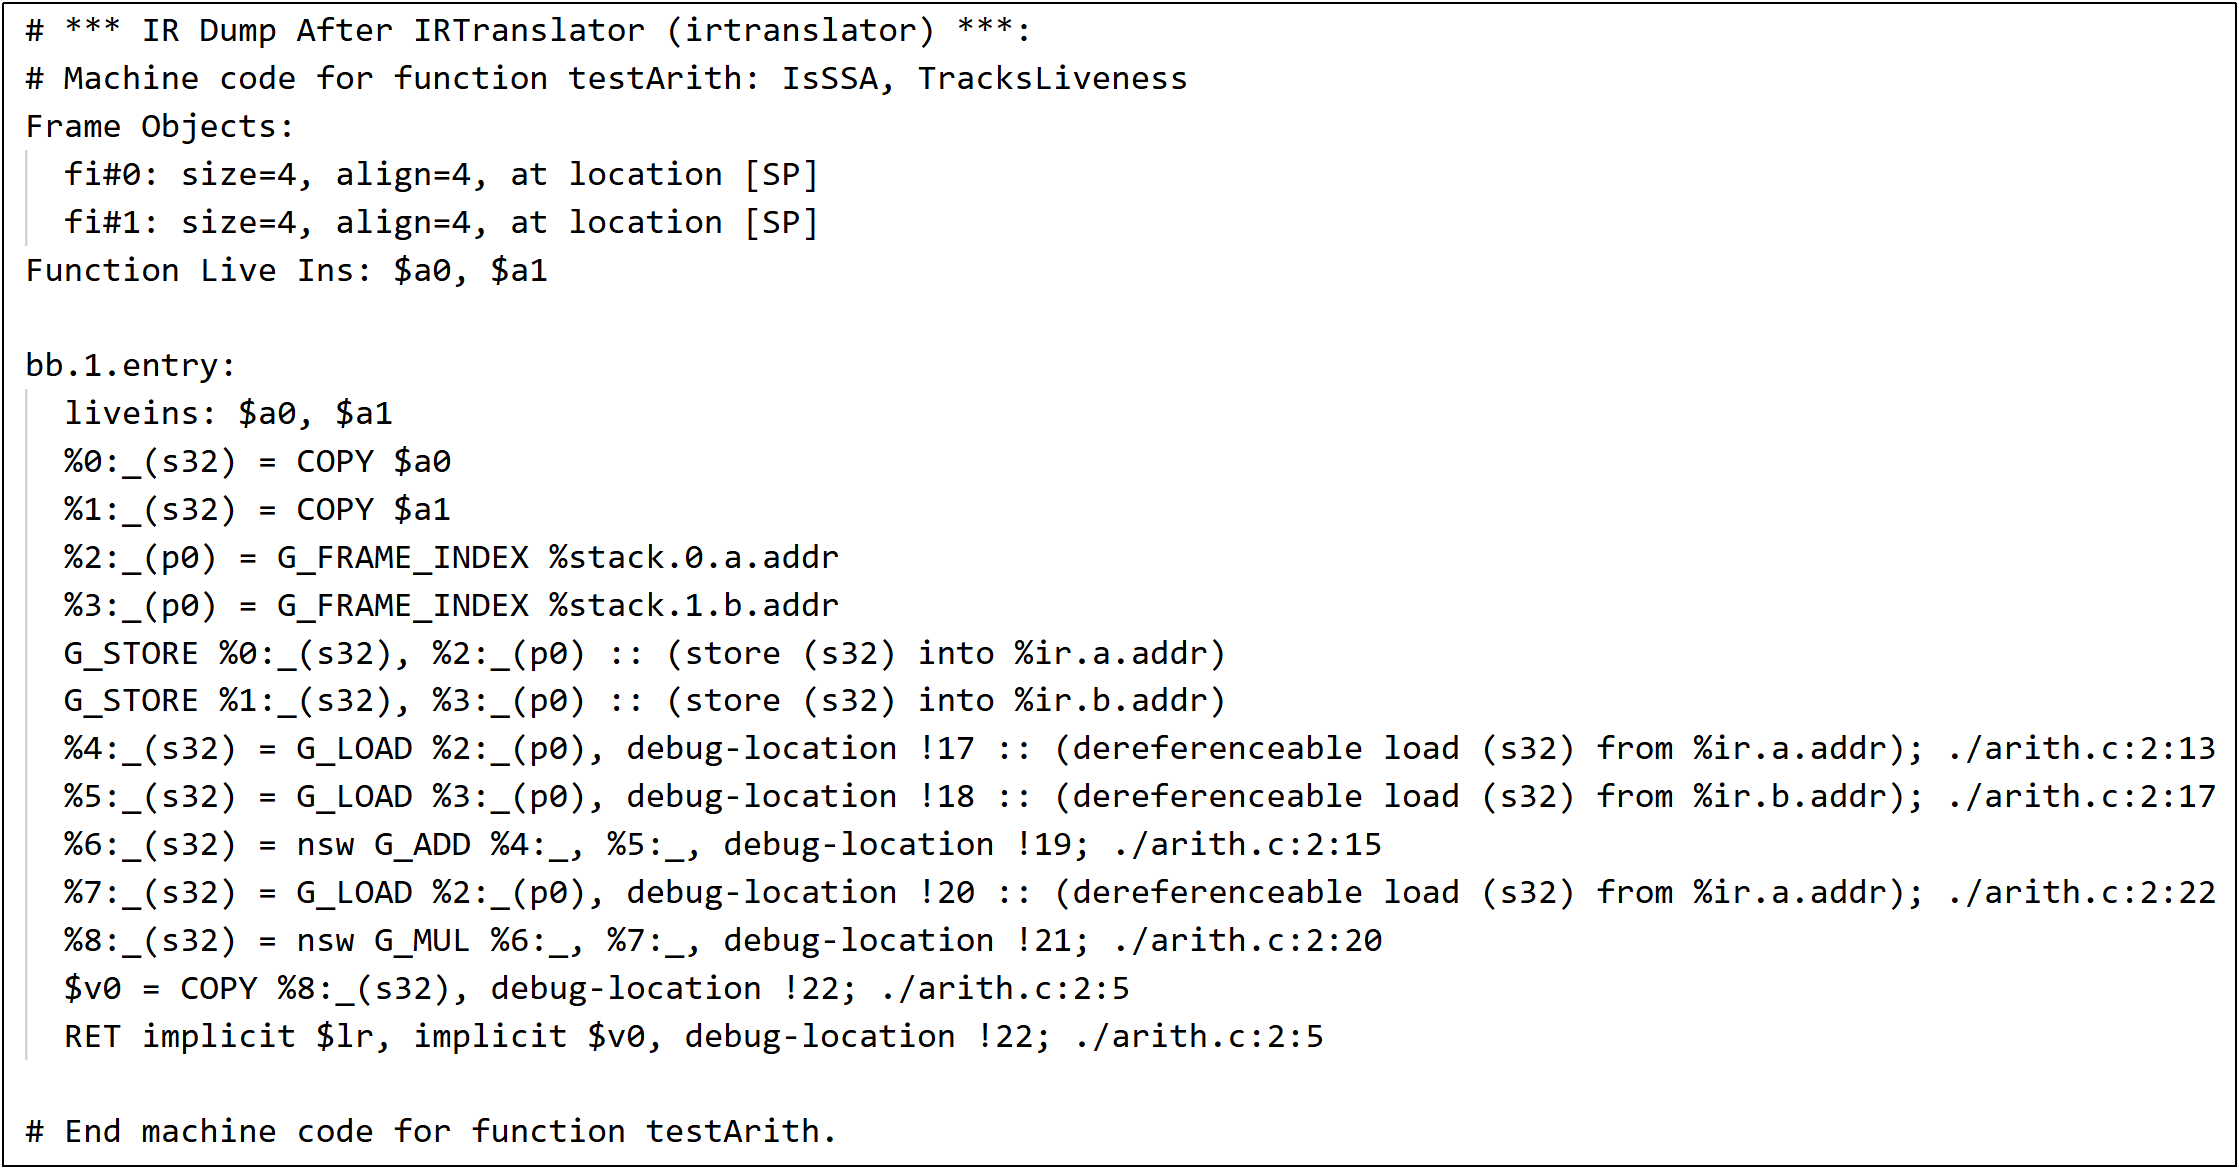
\includegraphics[width=1\textwidth]{pics/case_1_gmir_gen_dump.png}
	\caption{示例一GMIR生成阶段Dump图}
	\label{fig:case_1_gmir_gen_dump}
\end{figure}

该结果表明,LLVM IR到GMIR的转换过程保持了原有运算语义与数据依赖关系,为后续后端处理提供了正确的输入。

3.合法化阶段

合法化阶段的主要任务是将GMIR中不被目标架构直接支持的指令形式,转换为目标架构可处理的合法形式。由于32bit的G\_ADD、G\_MUL、G\_LOAD和G\_STORE指令在DSP架构下均为合法操作,于是示例中并未触发类型扩展、分裂或指令拆分等复杂合法化操作。如图\ref{fig:case_1_legalize_dump}所示,合法化前后指令结构保持一致,说明DSP的合法化规则能够正确覆盖基本算术与内存访问指令。

\begin{figure}[htbp]
	\centering
	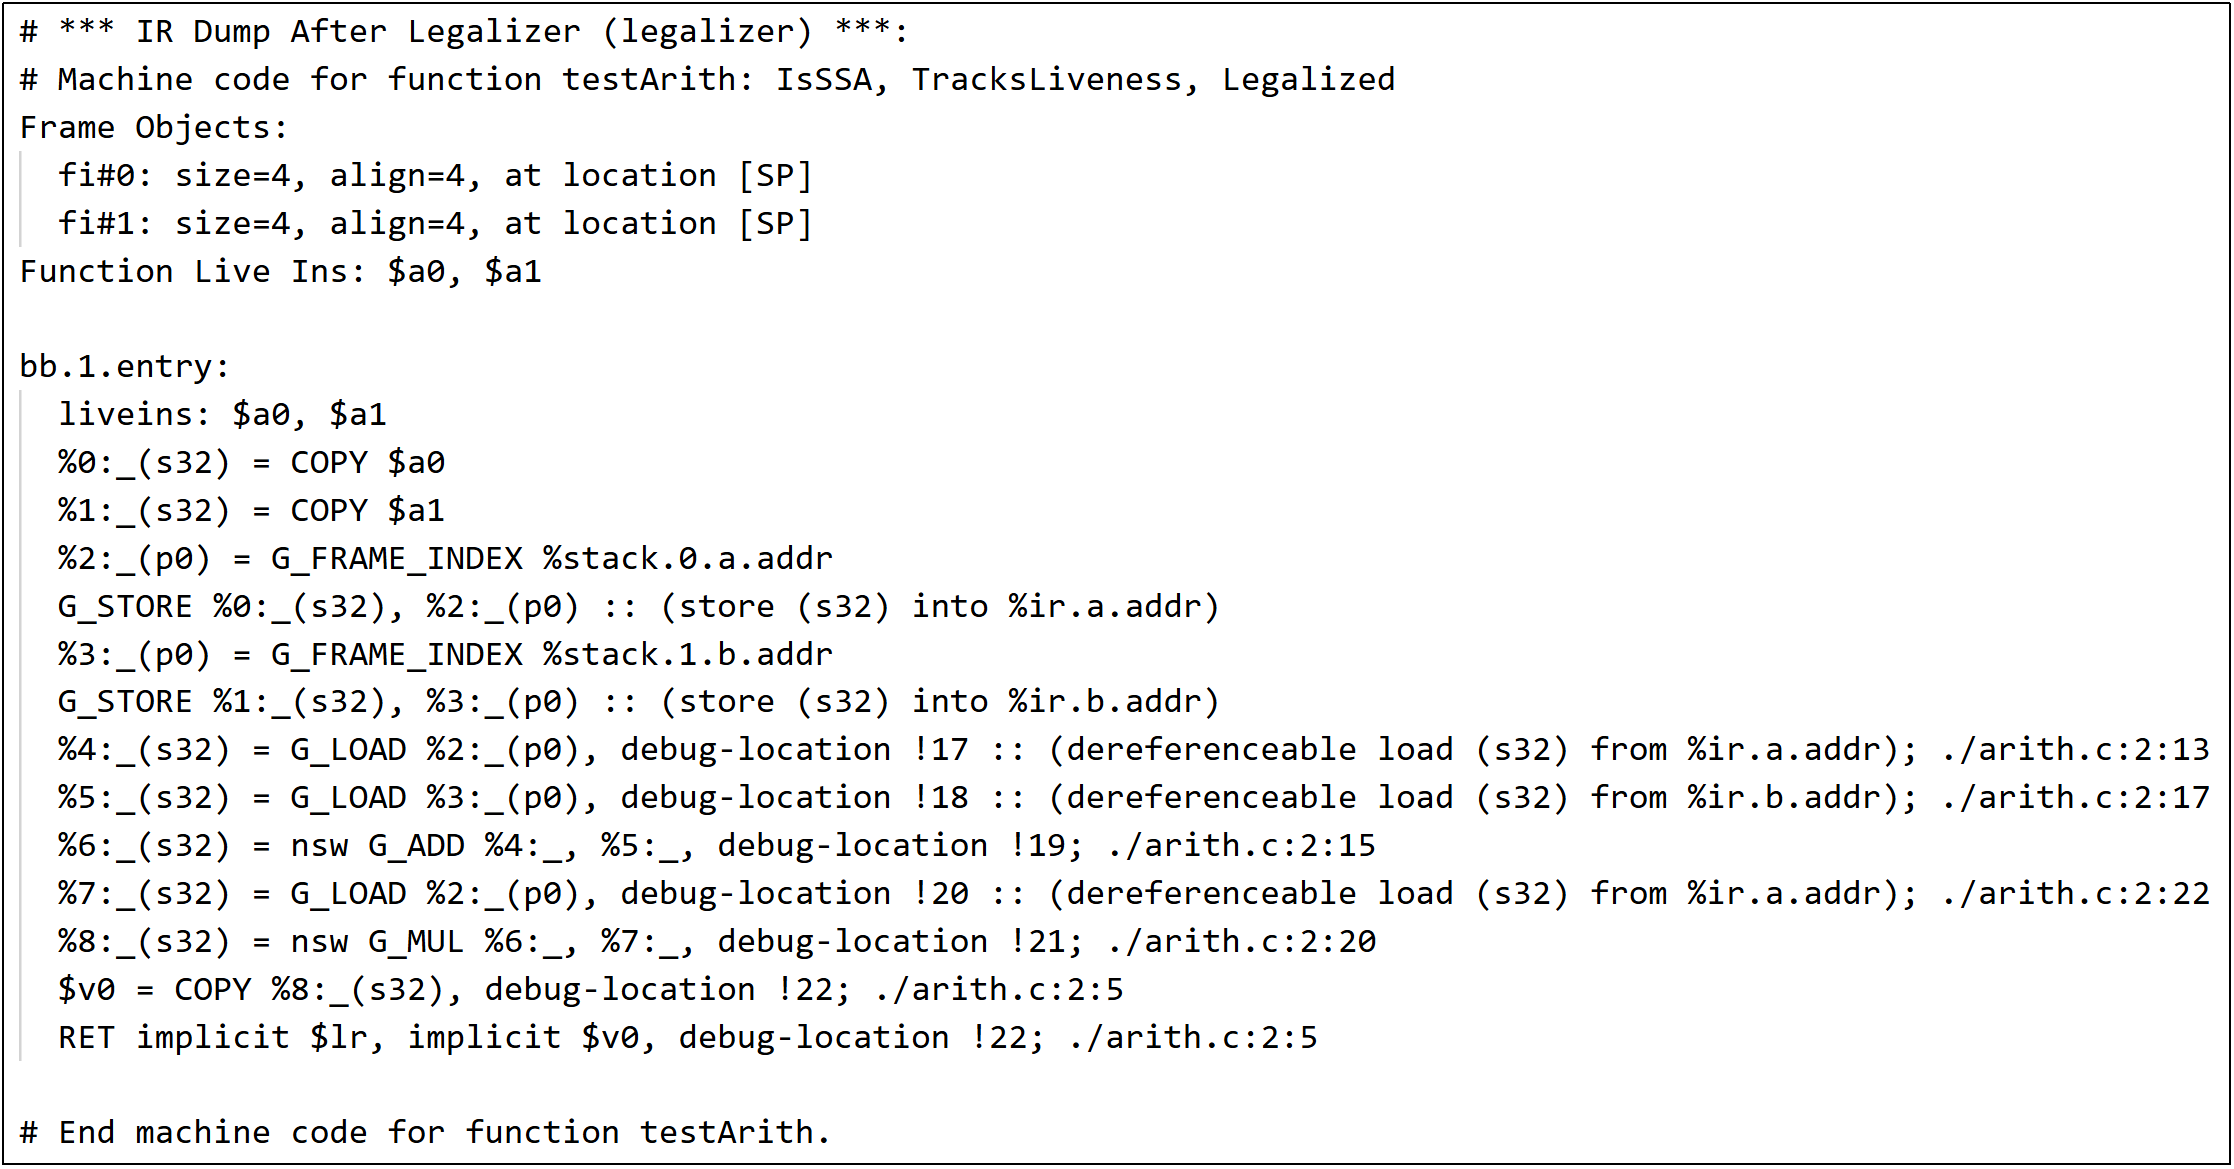
\includegraphics[width=1\textwidth]{pics/case_1_legalize_dump.png}
	\caption{示例一合法化阶段Dump图}
	\label{fig:case_1_legalize_dump}
\end{figure}

4.寄存器组选择阶段

在寄存器组选择阶段,编译器为每个虚拟寄存器分配合适的寄存器组。在DSP后端中,参与整数算术运算的虚拟寄存器统一映射至通用整数寄存器组GPRB。如图\ref{fig:case_1_regbank_select_dump}所示,从寄存器组选择后的Dump结果可以观察到,所有算术指令的操作数及结果均被分配到GPRB寄存器组,且寄存器类型与操作数位宽保持一致。

\begin{figure}[htbp]
	\centering
	\includegraphics[width=1\textwidth]{pics/case_1_regbank_select_dump.png}
	\caption{示例一寄存器组选择阶段Dump图}
	\label{fig:case_1_regbank_select_dump}
\end{figure}

该结果表明所有参与算术运算的虚拟寄存器均被正确分配至通用寄存器组,同时未引入额外的跨寄存器组数据复制或冗余中间指令。

5.机器指令选择阶段

在机器指令选择阶段,GMIR被转换为DSP架构的目标机器指令。如\ref{fig:case_1_instr_select_dump}所示,从Dump结果可以观察到所有中间指令(除COPY外,需要在后续Pass中单独处理)都被正确的映射到DSP后端机器指令。

\begin{figure}[htbp]
	\centering
	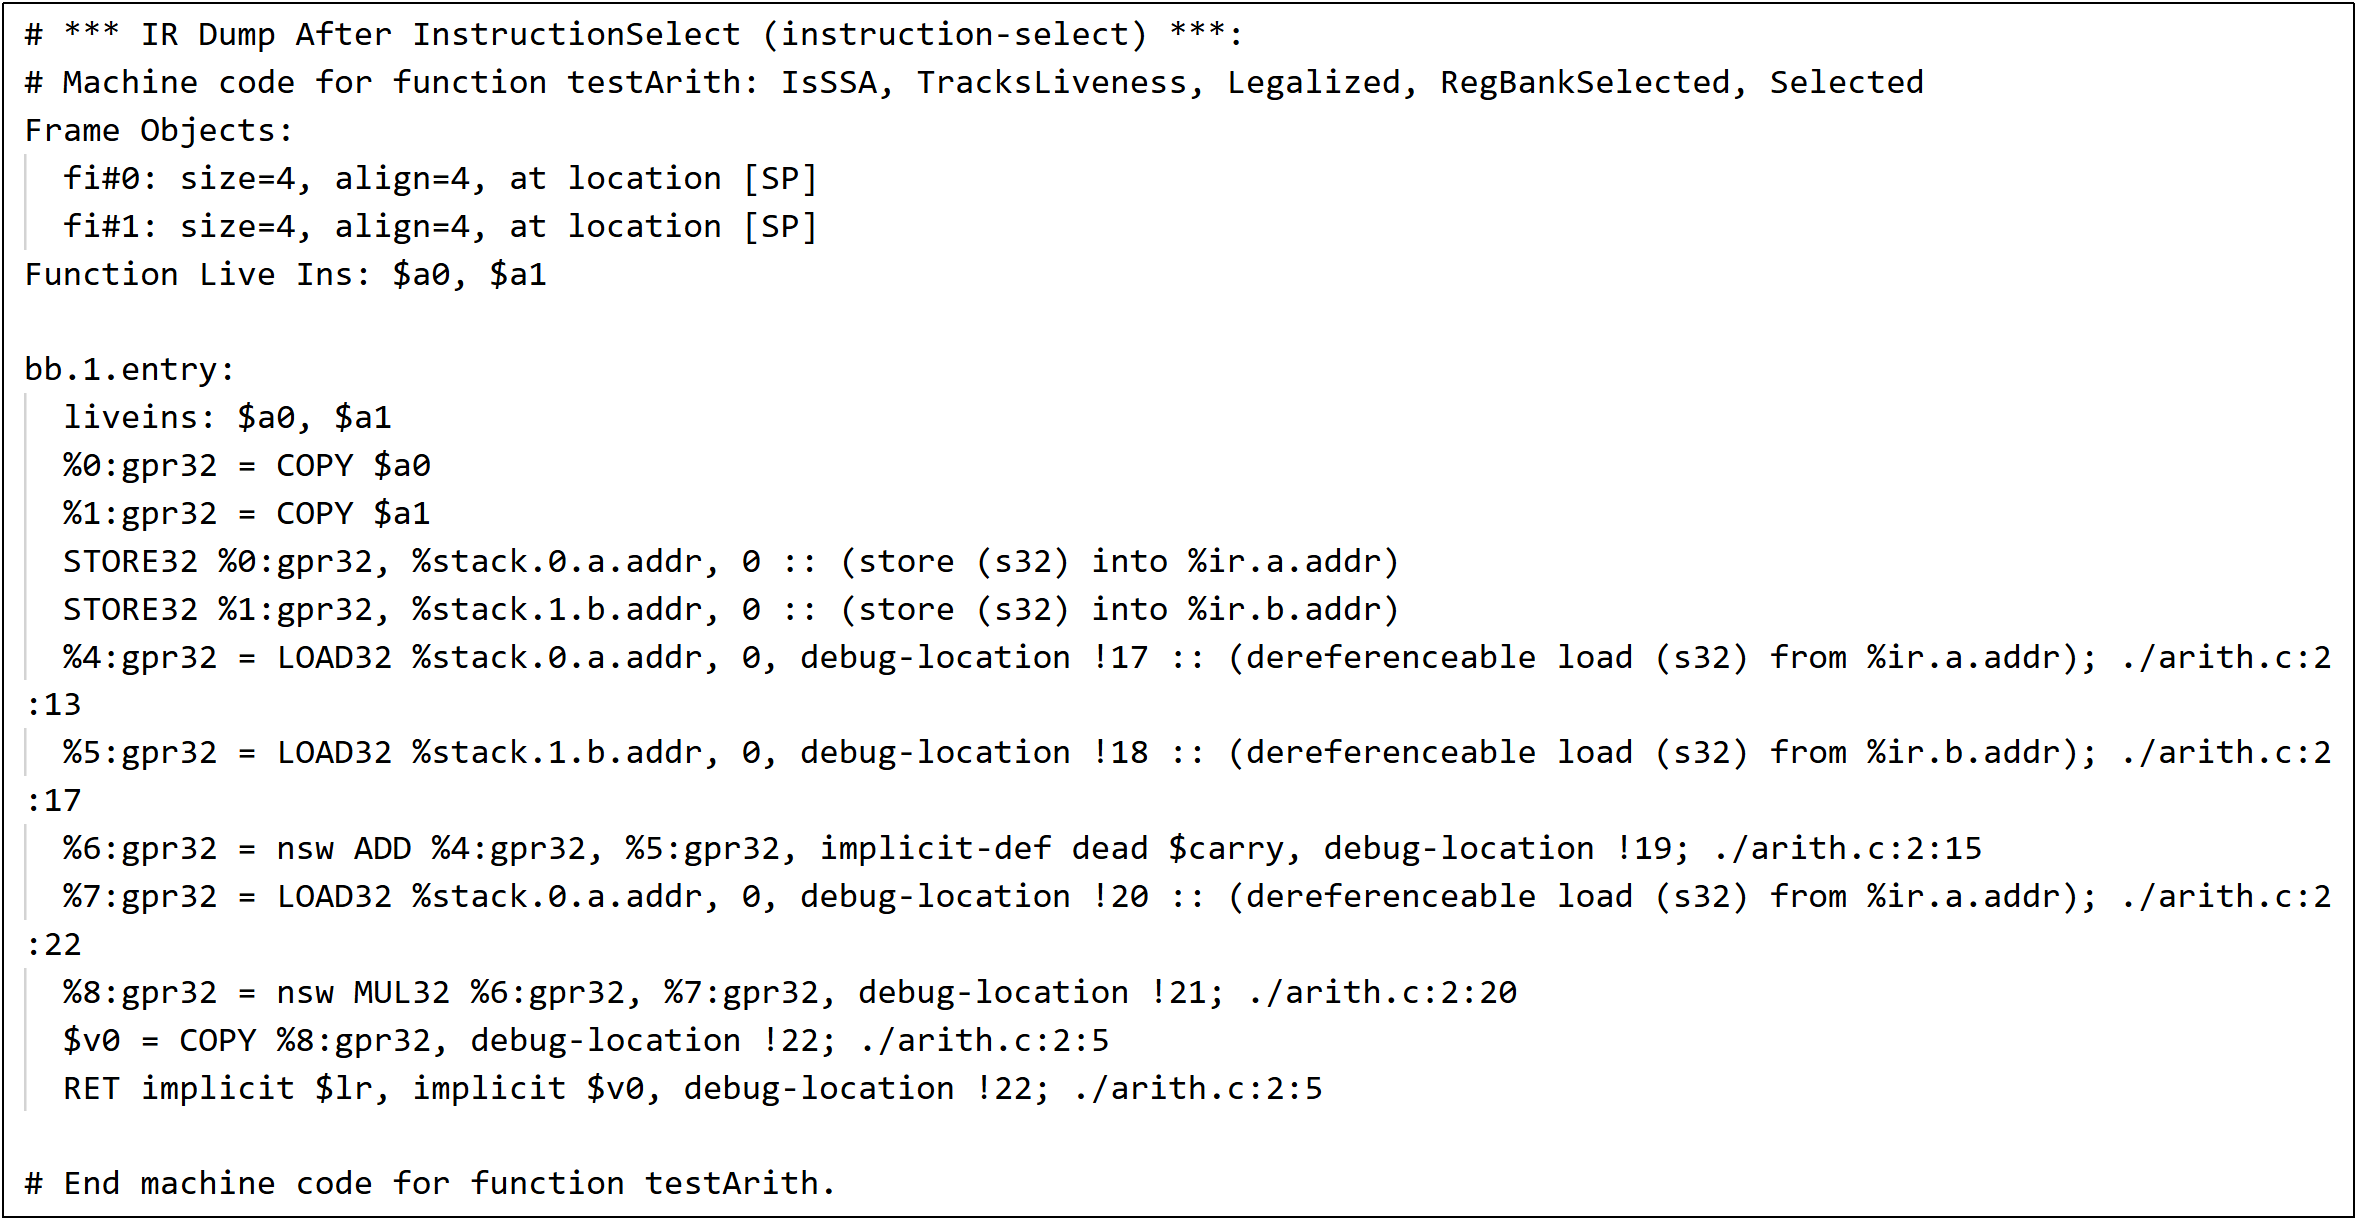
\includegraphics[width=1\textwidth]{pics/case_1_instr_select_dump.png}
	\caption{示例一机器指令选择阶段Dump图}
	\label{fig:case_1_instr_select_dump}
\end{figure}

6.最终代码生成

在经过寄存器分配、指令调度等后续后端Pass处理后,最终生成合法且可执行的DSP机器码。如图\ref{fig:case_1_final_dump}所示,整体代码生成流程未出现语义偏差或异常,验证了基本指令在GlobalISel框架下的端到端正确性。

\begin{figure}[htbp]
	\centering
	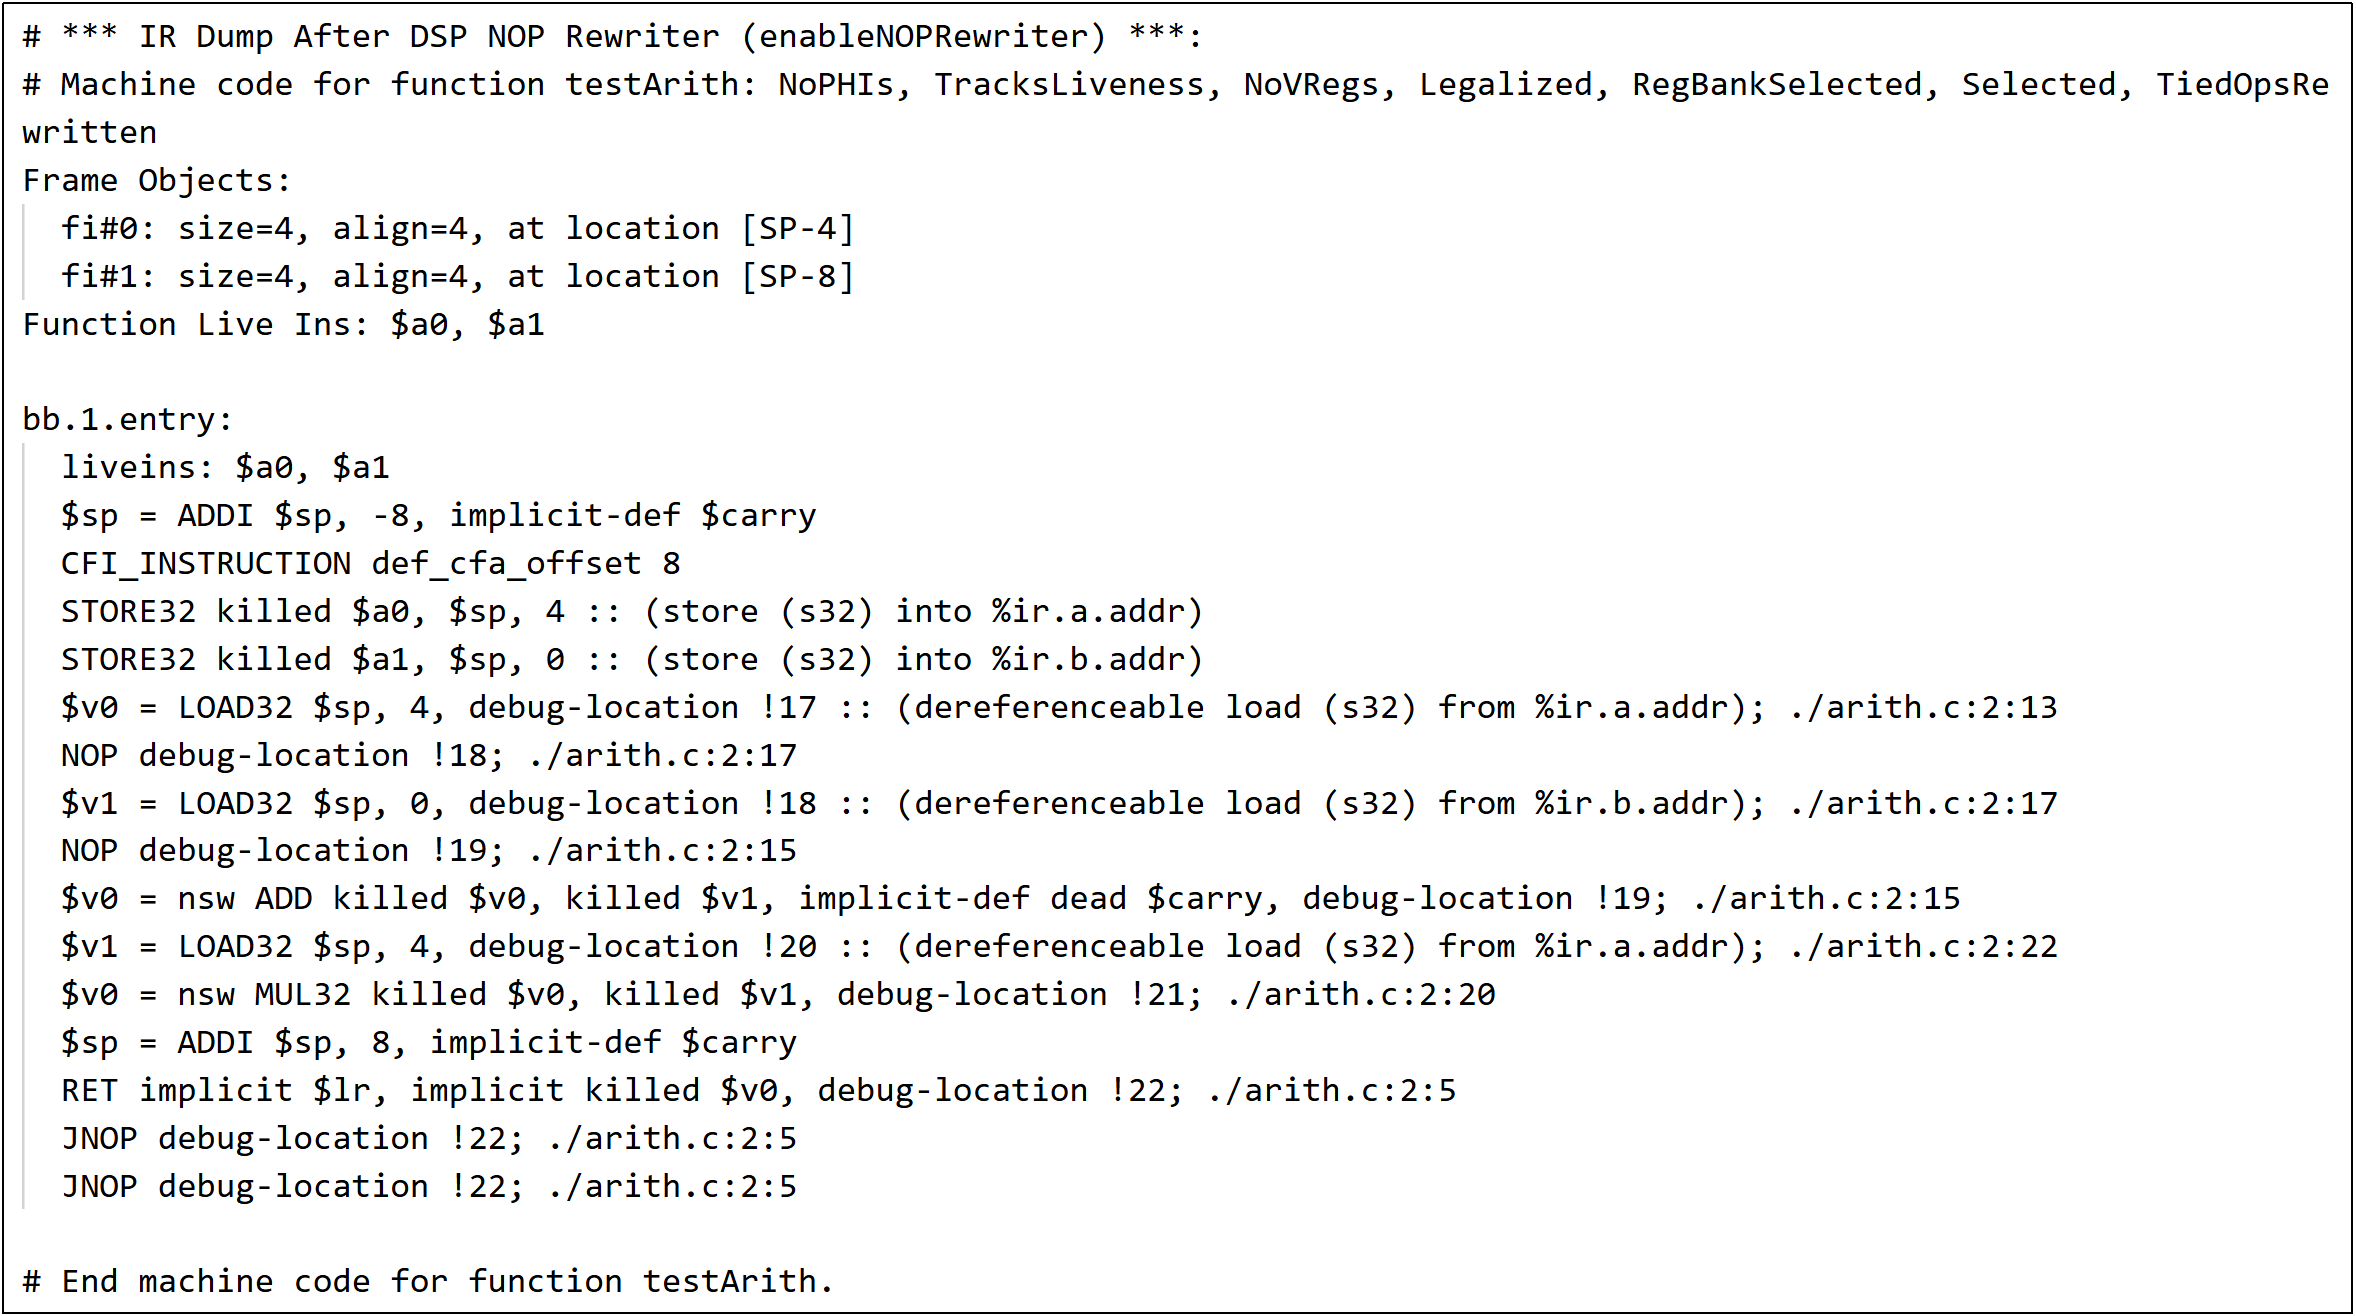
\includegraphics[width=1\textwidth]{pics/case_1_final_dump.png}
	\caption{示例一最后阶段Dump图}
	\label{fig:case_1_final_dump}
\end{figure}


% 5.1.2 控制流指令正确性验证
\subsection{控制流指令正确性验证}
除基本算术与内存访问指令这些基本指令外,控制流指令的正确生成和映射同样是验证编译器后端正确性的重要体现。本节针对对控制流相关指令的处理过程进行验证,重点覆盖比较与条件分支、循环结构以及函数调用三类典型控制流场景。

\par

1.比较+分支+跳转指令

比较与条件分支是程序控制流构建的基础。在LLVM IR中,该类操作通常通过icmp与br指令组合表达;在GlobalISel框架下,则对应为G\_ICMP与G\_BRCOND等GMIR指令。为验证DSP后端对该类控制流指令的处理正确性,本文构建了一个同时包含比较、条件分支及无条件跳转的示例二,其LLVM IR如下所示:

\lstset{language=c++}
\begin{lstlisting}
define dso_local i32 @testBranch() {
	entry:
	%retval = alloca i32
	%a = alloca i32
	%b = alloca i32
	store i32 10, ptr %a
	store i32 20, ptr %b
	%0 = load i32, ptr %a
	%1 = load i32, ptr %b
	%cmp = icmp slt i32 %0, %1
	br i1 %cmp, label %if.then, label %if.else
	
	if.then:
	store i32 0, ptr %retval
	br label %return
	
	if.else:
	store i32 1, ptr %retval
	br label %return
	
	return:  %2 = load i32, ptr %retval
	ret i32 %2
}
\end{lstlisting}

针对该示例,在GlobalISel各关键阶段中的处理过程如下:

\begin{itemize}
	\item
	在GMIR生成阶段,LLVM IR中的比较指令被正确转换为G\_ICMP,其比较谓词与操作数保持一致;条件跳转指令被转换为G\_BRCOND,并以比较结果作为分支条件。
	
	\item
	在合法化阶段,由于DSP架构支持整数比较操作,无需进一步拆分,相关指令保持原有结构。
	
	\item 
	在寄存器组选择阶段,编译器为比较操作及其结果所涉及的虚拟寄存器分配了合适的寄存器组,确保比较结果能够以符合DSP架构约定的方式参与后续控制流指令。
	
	\item 
	在机器指令选择阶段,G\_ICMP与后续的G\_BRCOND会被联合处理,映射为DSP架构下的比较指令与条件跳转指令,比较结果通过条件码寄存器传递,从而完成分支控制。
	
\end{itemize}

如图\ref{fig:case_2_final_dump}所示,在函数入口基本块中,比较指令首先生成条件码寄存器状态,随后通过条件跳转指令根据比较结果在两个后继基本块之间进行分支选择,验证了比较与条件分支指令的正确映射。

\begin{figure}[htbp]
	\centering
	\includegraphics[width=1\textwidth]{pics/case_2_final_dump.png}
	\caption{示例二入口基本块最后阶段Dump图}
	\label{fig:case_2_final_dump}
\end{figure}

如图\ref{fig:case_2_final_dump_2}所示,条件分支后的if.then与if.else基本块分别执行对应路径逻辑,并通过无条件跳转汇合至统一的返回基本块。最终生成的机器码中,各分支路径与返回块之间的控制流关系与LLVM IR描述保持一致。

\begin{figure}[htbp]
	\centering
	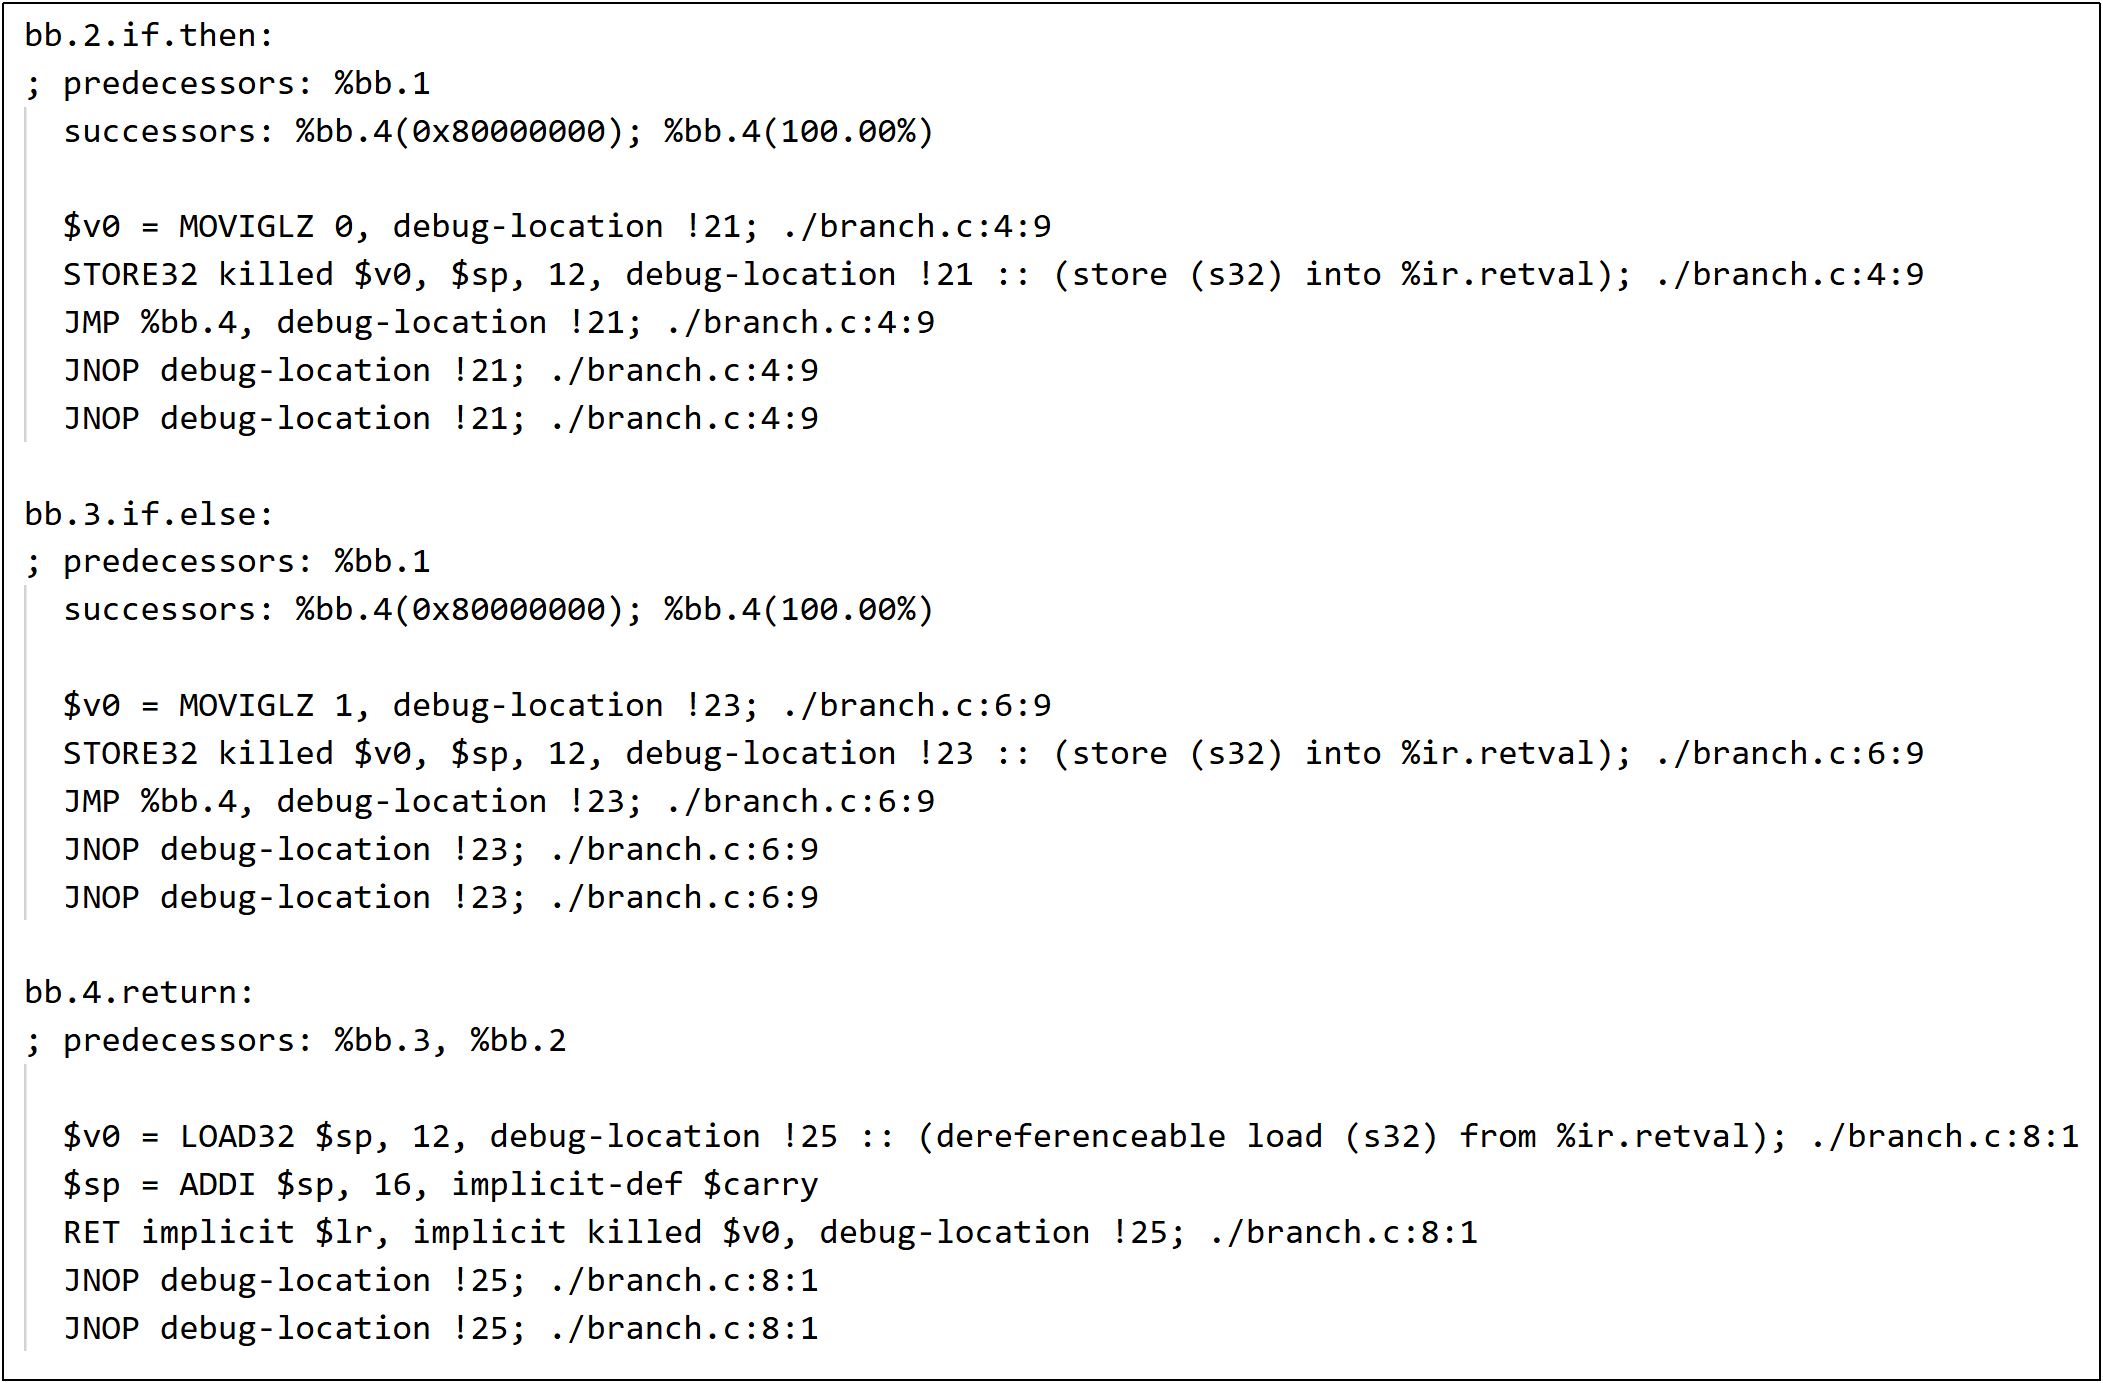
\includegraphics[width=1\textwidth]{pics/case_2_final_dump_2.png}
	\caption{示例二条件分支基本块最后阶段Dump图}
	\label{fig:case_2_final_dump_2}
\end{figure}

实验结果表明,从LLVM IR到最终机器码的转换过程中,比较条件与分支目标均保持一致,程序控制流未发生偏移或错误跳转,验证了比较与分支指令选择的正确性。

\par

2.循环指令

循环结构通常由条件判断、分支跳转以及回边构成,是控制流指令组合应用的典型场景。在LLVM IR中,循环通过多个基本块以及br指令共同表示;在GMIR层面,该多基本块结构及其控制流关系被完整保留下来,为后端代码生成提供了清晰的控制流语义。

\par

为验证DSP后端对循环指令的处理正确性,本文构建了一个包含循环指令的示例三,其LLVM IR如下所示:

\lstset{language=c++}
\begin{lstlisting}
define dso_local i32 @testLoop() {
	entry:
	%i = alloca i32
	store i32 0, ptr %i
	br label %for.cond
	
	for.cond:
	%0 = load i32, ptr %i
	%cmp = icmp slt i32 %0, 10
	br i1 %cmp, label %for.body, label %for.end
	
	for.body:
	br label %for.inc, !dbg !21
	
	for.inc:
	%1 = load i32, ptr %i
	%inc = add nsw i32 %1, 1
	store i32 %inc, ptr %i
	br label %for.cond
	
	for.end:
	ret i32 0
}
\end{lstlisting}

针对该示例,在GlobalISel各关键阶段中的处理过程如下:

\begin{itemize}
	\item
	在GMIR生成阶段,各基本块及其控制流关系被准确映射为MBB,循环条件与跳转关系通过G\_BR与G\_BRCOND指令表达。
	
	\item
	在合法化阶段,合法化前后指令结构保持一致,表明DSP后端的合法化规则能够覆盖该类循环场景的基本操作需求。
	
	\item 
	在寄存器组选择阶段,循环体内的算术与内存操作被正确映射至DSP通用寄存器组,循环条件判断所依赖的比较结果亦能够被正确传播。
	
	\item 
	在机器指令选择阶段,循环控制流相关的G\_ICMP与G\_BRCOND被联合分析并映射为DSP架构下的比较指令与条件跳转指令:比较结果通过条件码寄存器生成,并由条件跳转指令读取实现分支决策。
	
\end{itemize}

如图\ref{fig:case_3_final_dump}所示,在循环条件基本块中,编译器首先对循环变量与上界进行比较,并通过条件码寄存器生成分支条件,随后依据比较结果在循环体与循环结束块之间进行跳转,验证了循环条件判断与分支决策逻辑的正确性。

\begin{figure}[htbp]
	\centering
	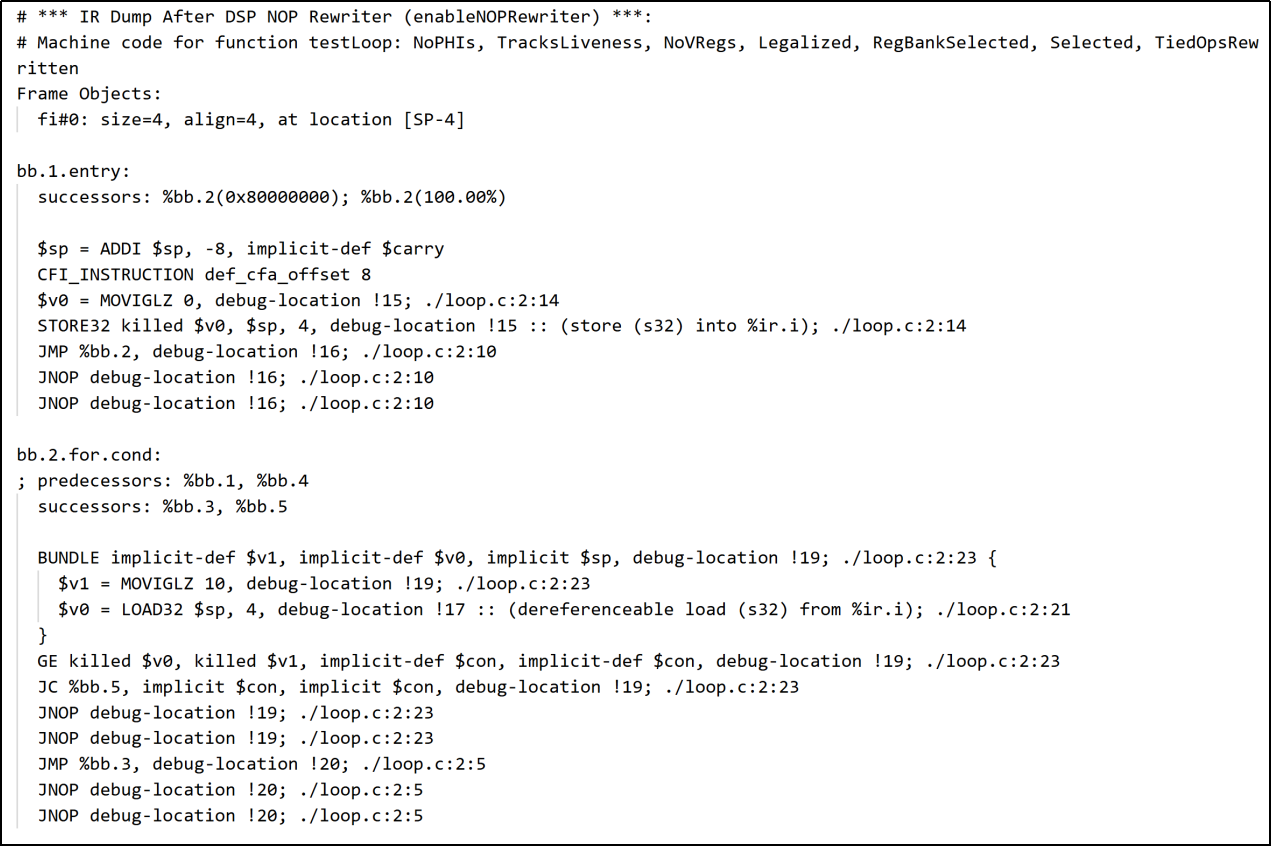
\includegraphics[width=1\textwidth]{pics/case_3_final_dump.png}
	\caption{示例三循环条件基本块最后阶段Dump图}
	\label{fig:case_3_final_dump}
\end{figure}


如图\ref{fig:case_3_final_dump_2}所示,循环体与自增基本块在执行完成后通过无条件跳转形成回边,并重新进入条件判断块;当循环条件不满足时,控制流正确跳转至循环结束块并完成函数返回,表明循环控制流在后端生成过程中保持一致。

\begin{figure}[htbp]
	\centering
	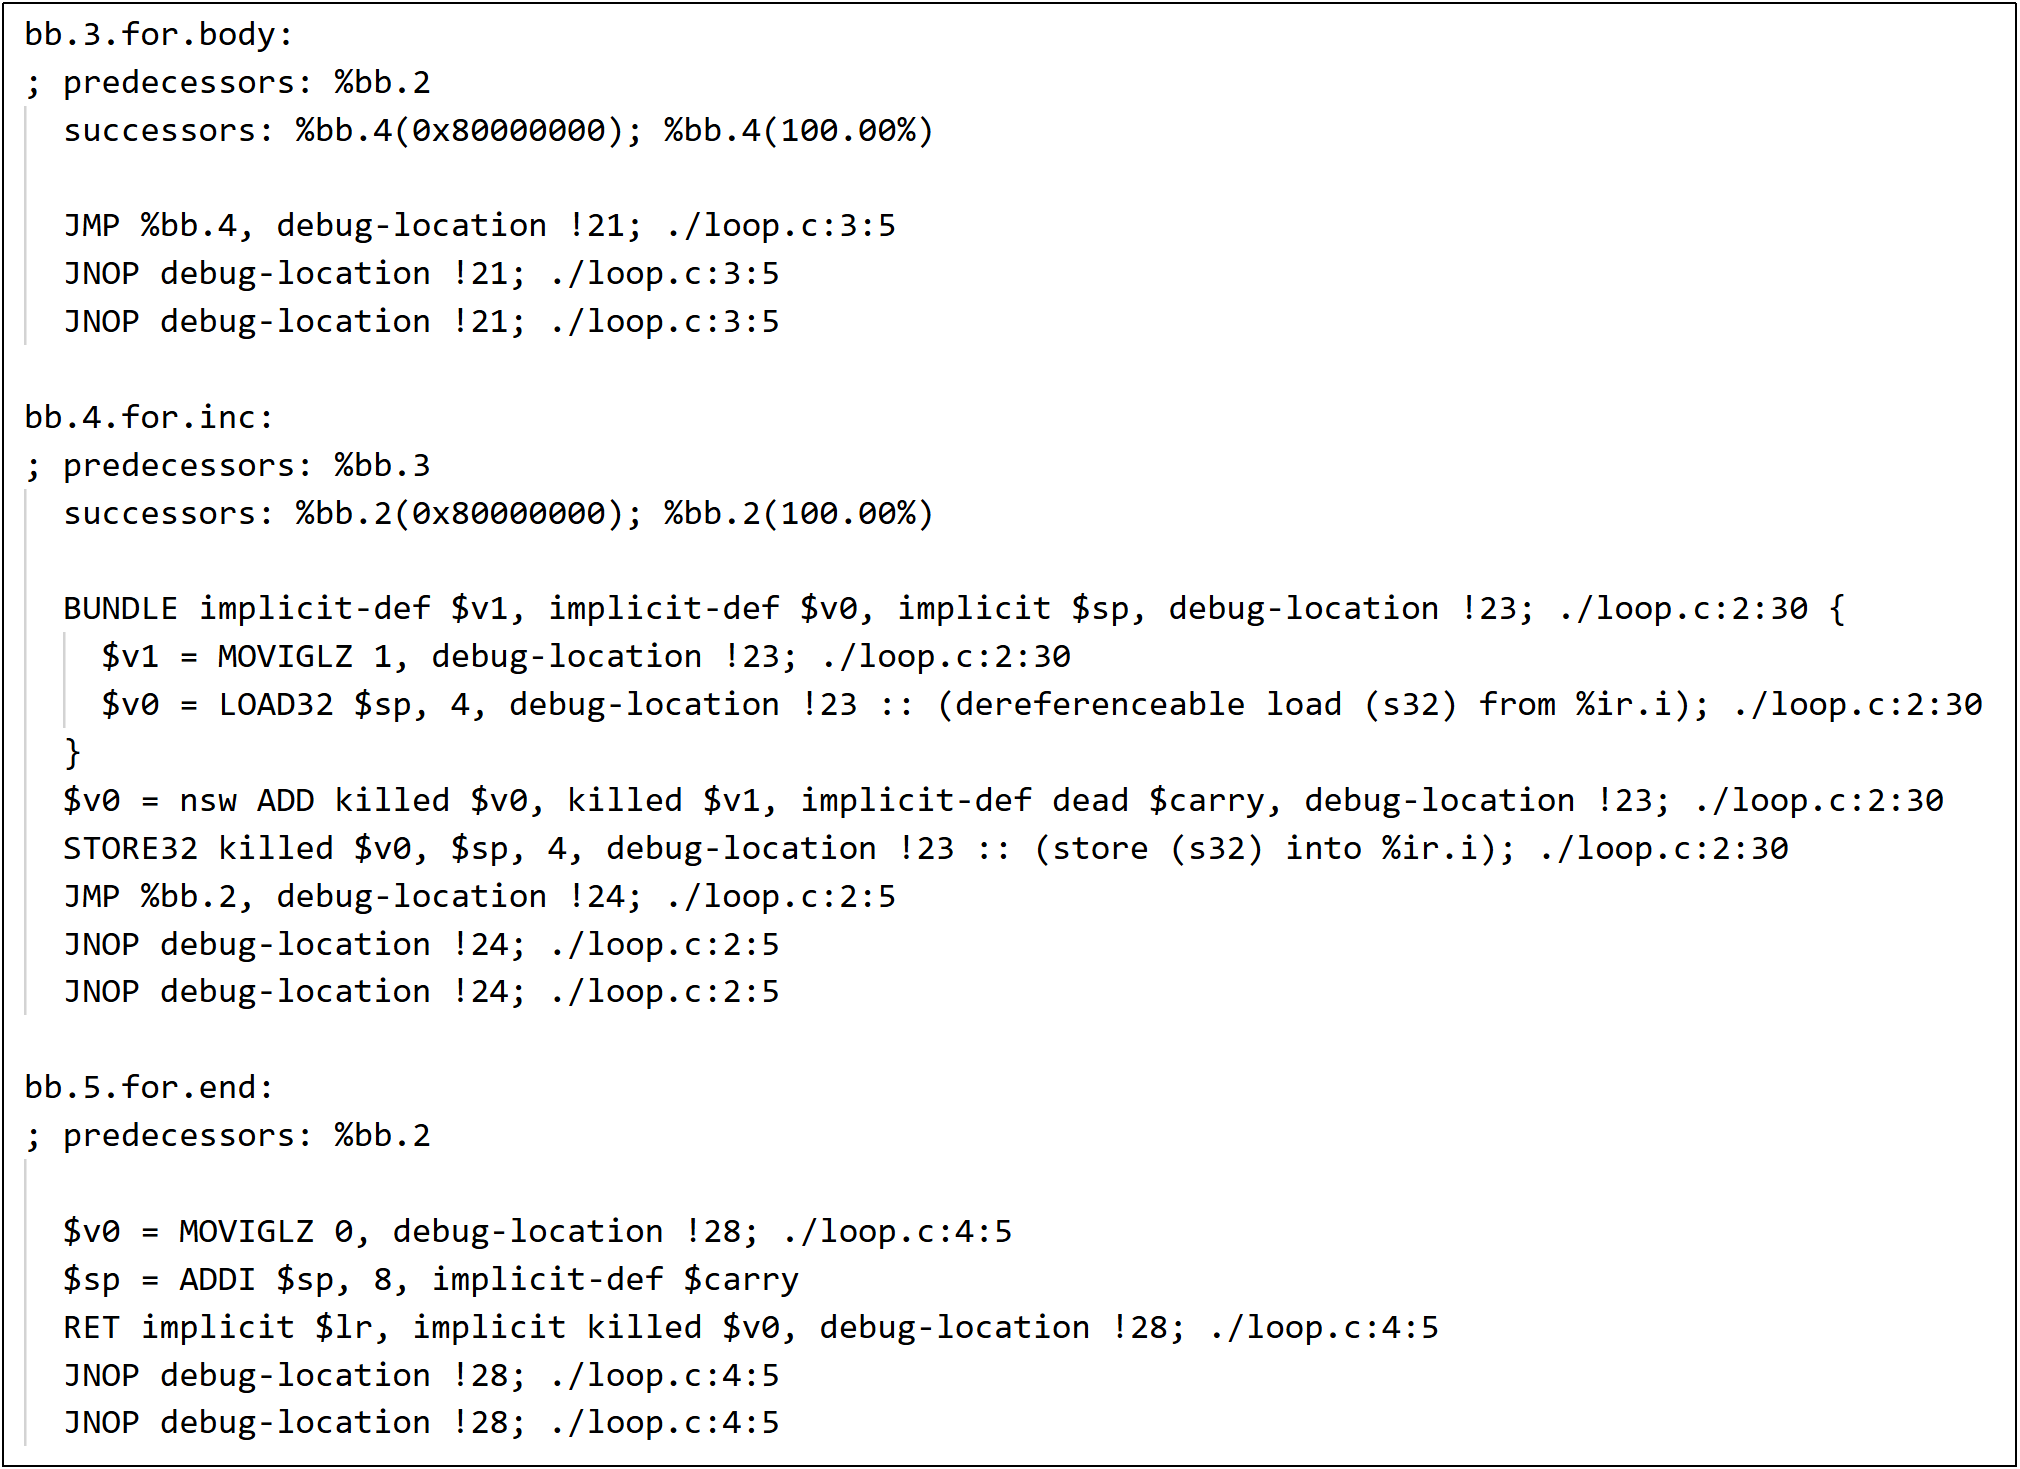
\includegraphics[width=1\textwidth]{pics/case_3_final_dump_2.png}
	\caption{示例三循环体基本块最后阶段Dump图}
	\label{fig:case_3_final_dump_2}
\end{figure}


从最终生成的机器码可以观察到,循环入口、循环体以及循环回边对应的跳转指令均与原始LLVM IR的控制流结构保持一致,且不存在多余或缺失的跳转指令。这表明GlobalISel在DSP后端中能够正确处理多基本块循环结构,确保循环语义的正确性。

\par

3.函数调用指令

函数调用是另一类重要的控制流操作,其正确性依赖于调用约定、参数传递以及返回值处理等多个方面。在LLVM IR中,函数调用通过call指令表示;在GlobalISel框架下,该过程涉及CallLowering与指令选择等多个阶段。

\par

为验证DSP后端在GlobalISel框架下对函数调用指令的处理正确性,构造了一个简单的示例四,其中main函数调用前文定义的testBranch函数,其LLVM IR如下所示:

针对该示例函数,函数调用在各阶段的处理过程如下:

\begin{itemize}
	\item
	在GMIR生成阶段,call指令被转换为一系列与调用约定相关的GMIR指令,包括参数准备、调用指令以及返回值接收等操作。
	
	\item
	在合法化阶段,合法化前后指令结构保持一致,表明DSP后端的合法化规则能够覆盖该类函数调用场景的基本操作需求。
	
	\item 
	在寄存器组选择阶段,函数参数与返回值被分配至DSP架构规定的寄存器或栈位置,符合DSP ABI的约定规则。
	
	\item 
	在机器指令选择阶段,调用相关的GMIR指令被映射为DSP架构支持的跳转与返回指令,并正确维护返回地址与调用现场。最终生成的机器码中,函数调用前后的寄存器状态与栈帧布局保持一致,函数返回值能够被正确读取并参与后续计算。
	
\end{itemize}

如图\ref{fig:case_4_final_dump}所示,实验结果表明DSP后端在GlobalISel框架下能够正确完成函数调用相关控制流的指令选择,保证跨函数控制流的正确传递。

\begin{figure}[htbp]
	\centering
	\includegraphics[width=1\textwidth]{pics/case_4_final_dump.png}
	\caption{示例四最后阶段Dump图}
	\label{fig:case_4_final_dump}
\end{figure}


%*********************************************************************
% 5.2 全局指令选择性能分析
%*********************************************************************
\section{全局指令选择性能分析}
本章主要针对编译时间、代码大小以及执行周期三个方面来对基于DAG的指令选择、未优化的全局指令选择以及优化的全局指令选择来进行对比。


% 5.2.1 编译时间
\subsection{编译时间}
编译时间是衡量编译器工程可用性与开发效率的重要指标之一,尤其在编译器持续迭代与频繁回归验证的场景下,后端编译开销的变化将直接影响开发效率与测试周期。因此,本节围绕编译时间这一维度,对不同指令选择方案在DSP后端中的表现进行系统对比分析。

1.度量方法与相关指标说明

本文的编译时间的量化分析基于Clang自带的编译时间追踪机制,该机制能够对编译过程中各阶段的执行时间进行精细化统计,从而为分析编译器性能瓶颈与优化效果提供可靠的数据支撑。图\ref{fig:compile_time_example}中展示了部分关键时间指标及其在不同编译阶段的分布情况。

\begin{figure}[htbp]
	\centering
	\includegraphics[width=1\textwidth]{pics/compile_time_example.png}
	\caption{不同编译阶段时间指标图}
	\label{fig:compile_time_example}
\end{figure}

其中,各时间指标的含义如下:

\begin{itemize}
	\item
	User Time(用户态时间):表示CPU在用户态执行编译器自身代码所消耗的时间,仅反映编译器逻辑计算的开销,不包含操作系统内核相关操作。
	
	\item
	System Time(系统态时间):表示CPU在内核态执行系统调用(如文件读写、内存管理、进程调度等)所消耗的时间,属于编译过程中的系统辅助开销。
	
	\item 
	User+System Time(用户态加系统态时间):反映CPU在该阶段用于计算的总耗时,是用户态和系统态时间的累加,但不包含I/O等待和CPU空闲时间。
	
	\item 
	Wall Time(壁钟时间):指从编译阶段开始到结束所经历的实际物理时间,包含CPU计算、I/O等待、进程调度以及资源竞争等所有因素。在真实工程场景中,该指标最能直观反映用户实际感知到的编译等待时长,因此也是本文关注的核心量化指标。
	
\end{itemize}

LLVM编译流程可粗略划分为以下几个阶段:

\begin{itemize}
	\item
	Front end(前端):包括源代码解析、语法分析、语义分析等操作,主要负责将高级语言代码转换为中间表示。
	
	\item
	LLVM IR generation(LLVM IR生成):将前端分析结果转换为LLVM中间表示,为后续优化和代码生成奠定基础。
	
	\item 
	Optimizer(优化器):对LLVM IR进行多级优化,包括控制流优化、数据流优化及目标无关优化等。
	
	\item 
	Machine code generation(机器码生成):编译器后端的核心阶段,负责指令选择、寄存器分配、指令调度以及最终目标机器码的生成。
	
\end{itemize}

由于指令选择阶段在LLVM后端中与其他流程高度耦合,难以单独抽离并进行精确量化,因此本文在编译时间分析中,将关注点放在后端整体执行时间上。具体而言,仅统计Machine Code Generation阶段的Wall Time,以此作为后端编译开销的统一度量标准。该统计方式在保证分析结果可比性和稳定性的同时,能够有效反映后端相关优化对实际编译时间的影响,为后续性能评估提供依据。

2.实验设置与统计方法

实验基于Embench测试集进行。为降低单次测量中噪声与偶然因素对实验结果的影响,本文采用多次重复实验的统计方法:在相同实验环境与配置条件下,对每个测试样例分别执行10次编译;在结果统计阶段,剔除两个最大值和两个最小值,对剩余数据取平均值作为该样例在对应优化等级下的编译时间;随后,对Embench测试集中22个基准程序的结果进一步取平均,得到不同优化等级下的平均编译时间,用于不同指令选择方案之间的对比分析。

3.实验结果与分析

图\ref{fig:compile_time_contrast}给出了在Embench测试集上两种指令选择方案在不同优化等级下的平均编译时间对比结果。

\begin{figure}[htbp]
	\centering
	\includegraphics[width=1\textwidth]{pics/compile_time_contrast.png}
	\caption{两种指令选择方案平均编译时间对比图}
	\label{fig:compile_time_contrast}
\end{figure}

从图中可以观察到,在四个优化等级下,GlobalISel均表现出更低的平均编译时间。该趋势在O0与O1等低优化等级下尤为明显,表明在中端优化尚未充分展开的情况下,指令选择框架自身的设计差异已对后端编译效率产生显著影响。这一结果主要源于GlobalISel在指令选择阶段采用的基于规则匹配与直接构造Machine IR的流程,相较于传统基于DAG的指令选择方式,其构建与遍历成本更低,整体流程更为线性。此外,GlobalISel在GMIR层面引入的早期规范化与合并优化,也在一定程度上减少了后续Pass的处理负担,从而降低了整体后端编译开销。

4.实验结论

综合实验结果可以得出结论:在DSP后端中,GlobalISel相较于SelectionDAG在编译时间维度上具有稳定优势。该优势在不同优化等级下均保持一致,说明其并非依赖特定优化配置,而是来源于指令选择框架本身在流程设计与中间表示处理上的效率改进。这一特性使得GlobalISel更适合于需要频繁编译与快速迭代的工程场景,为后续编译器优化与性能验证提供了良好的基础。


% 5.2.2 代码尺寸
\subsection{代码尺寸}
代码尺寸是衡量编译器后端代码生成质量的重要指标之一,尤其在DSP等嵌入式场景中,程序存储空间受限,指令密度直接影响系统可部署规模与功耗水平。因此,分析不同指令选择方案对最终生成代码体积的影响,对于评估GlobalISel优化效果具有重要意义。

1.度量方法

本文的代码尺寸的量化基于llvm-size工具完成,并以目标文件中text段大小作为代码尺寸的度量指标。该指标能够直接反映指令选择与代码生成阶段所产生的指令数量与编码密度,同时有效规避调试信息、符号表等非执行内容对统计结果的干扰。

\par

2.实验设置与统计方法

在实验设置上,本文基于Embench测试集,对每个基准程序分别在四个优化等级下进行编译,并统计对应生成目标文件的text段大小。对于同一测试样例与优化等级,取单次编译结果作为该样例的代码尺寸;随后,对测试集内所有基准程序的结果取平均值,得到各优化等级下的平均代码段尺寸,用于不同指令选择方案之间的对比分析。


3.实验结果分析

图\ref{fig:size_contrast}给出了在Embench测试集上,未引入优化的GlobalISel与引入优化后的GlobalISel在不同优化等级下的平均代码段尺寸对比结果。

\begin{figure}[htbp]
	\centering
	\includegraphics[width=1\textwidth]{pics/size_contrast.png}
	\caption{优化前后平均代码段尺寸对比图}
	\label{fig:size_contrast}
\end{figure}

从整体趋势来看,在四个优化等级下,优化后的GlobalISel方案均生成了更小的平均代码体积,且这一优势在O0等级下尤为明显。这表明,即使在未启用高层LLVM IR优化的情况下,后端针对指令选择与指令组合所引入的优化措施,仍然能够有效减少冗余指令并提升代码密度。高优化等级下,代码尺寸下降幅度相对收敛。这一现象表明,在高层LLVM IR优化充分展开后,部分冗余已在前端或中端被消除,后端指令选择优化对代码体积的影响更多体现为精细化的指令密度改进,而非数量级上的减少。

4.实验结论

综合实验结果可以得出结论:相较于未优化的GlobalISel实现,引入针对DSP架构特点的指令选择与指令组合优化后,编译器在各优化等级下均能够生成更紧凑的目标代码。这表明所提出的优化策略不仅在性能层面有效,同时也在代码尺寸这一关键指标上取得了稳定收益,为后续嵌入式场景中的实际部署提供了有力支撑。结合前文第3章中对优化策略的分析,可以将代码体积下降的原因归纳为以下几个方面:

\begin{itemize}
	\item
	冗余通用指令的提前消除
	通过在合法化前与合法化后引入针对GMIR的合并优化,显著减少了由类型拆分、表达式规范化以及中间表示泛化所引入的冗余指令,从而降低了最终生成指令的数量。
	
	\item
	目标相关指令模式的更充分匹配
	优化后的GlobalISel在指令选择阶段能够更有效地将通用指令序列映射为DSP架构提供的复合指令或更紧凑的指令形式,减少了多条通用指令展开带来的代码膨胀。
	
	\item 
	立即数与内存操作的定制化优化
	针对立即数装载与小规模内存操作引入的目标相关优化,避免了不必要的长立即数装载序列及库函数调用,进一步降低了代码体积。
	
\end{itemize}


% 5.2.3 执行周期
\subsection{执行周期}
执行周期是衡量编译器后端优化效果最直接、也是最具代表性的性能指标之一,尤其对于DSP等以吞吐率和实时性为核心设计目标的处理器架构而言,程序执行周期的变化能够直观反映指令选择、寄存器分配以及指令调度等后端决策对实际运行性能的影响。因此,本节围绕执行周期这一维度,对不同指令选择方案在DSP平台上的运行表现进行对比分析。

1.度量方法

本文的执行周期测量基于DSP工具链配套的仿真器环境完成。在仿真环境中,仿真器能够在程序执行过程中精确统计指令发射与执行情况,并直接给出程序完成所消耗的总周期数。

\par

为保证不同指令选择方案在执行周期统计上的可比性,本文在测量过程中统一采用相同的测试程序、输入数据以及运行环境配置,并仅关注程序主体计算阶段的执行周期,避免初始化、调试输出等非核心逻辑对统计结果产生干扰。最终得到的执行周期能够较为真实地反映编译器后端生成代码在DSP架构上的运行效率。

2.实验设置与统计方法

执行周期实验同样基于Embench测试集进行。对于每个基准程序,在相同硬件平台和配置条件下分别运行多次,以降低偶然扰动对测量结果的影响。具体统计方法如下:对每个测试样例在对应优化等级下执行10次,剔除两个最大值和两个最小值,对剩余结果取平均值作为该样例的执行周期;随后,对测试集中全部基准程序的执行周期结果进一步取平均,得到不同优化等级下的平均执行周期,用于不同指令选择方案之间的对比分析。

\par

该统计方式能够有效平衡测量精度与实验成本,在保证数据稳定性的同时,避免个别异常运行结果对整体趋势判断产生干扰。

3.实验结果与分析

图\ref{fig:cycle_contrast}给出了在Embench测试集上,不同指令选择方案在各优化等级下的平均执行周期对比结果。

\begin{figure}[htbp]
	\centering
	\includegraphics[width=1\textwidth]{pics/cycle_contrast.png}
	\caption{不同指令选择方案平均执行周期对比图}
	\label{fig:cycle_contrast}
\end{figure}

从实验结果可以观察到,相较于未优化的GlobalISel实现,引入针对DSP架构的指令选择与指令组合优化后,程序在所有优化等级下的平均执行周期均呈现出下降趋势。这表明,在高层LLVM IR优化与后端优化协同作用的场景中,GlobalISel所引入的目标相关指令匹配、冗余指令消除以及寄存器组绑定优化,能够进一步挖掘DSP架构的指令级并行潜力,从而在整体执行效率上获得持续收益。

\par

结合第3章中对优化策略的分析,可以将执行周期下降的主要原因归纳为以下几个方面:一是冗余通用指令在合法化前后被提前消除,减少了无效计算与不必要的数据搬移;二是优化后的指令选择能够更充分地利用DSP架构提供的复合指令与并行执行能力,提高了单周期内的有效计算密度;三是寄存器组选择与条件码处理策略的优化,降低了跨寄存器组复制与条件值传递带来的额外开销,从而缩短了关键路径长度。

4.实验结论

综合实验结果可以得出结论:在DSP后端中,引入针对目标架构特性的GlobalISel优化后,编译器生成代码在执行周期维度上取得了稳定且可观的性能提升。该提升在不同优化等级下均具有一致性,说明其并非依赖特定编译配置,而是源于指令选择框架与目标相关优化策略在整体设计上的协同改进。这一结果进一步验证了前文提出的优化方法在实际运行性能上的有效性,为后续章节中更细粒度的性能分析与应用验证奠定了基础。


%*********************************************************************
% 5.3 测试评估平台功能展示
%*********************************************************************
\section{测试评估平台功能展示}
测试评估平台围绕编译器工具链的持续迭代需求进行设计,集成了性能数据采集、历史回归分析、版本对比以及汇编级诊断等功能。平台通过对不同Commit在统一测试集上的性能表现进行系统化记录与分析,已在实际开发过程中协助发现并定位多个影响性能或代码生成质量的工具链缺陷,为编译器优化与回归验证提供了重要支撑。下文结合平台主要功能界面,详细展示其核心功能。

\par

1.全局性能趋势分析

如图\ref{fig:summary}所示,界面用于展示历史Commit的整体性能概览,侧重于从宏观层面分析编译器性能随时间的演进趋势。该界面基于完整测试集,对不同Commit下的平均代码体积和平均执行周期进行统计与可视化展示,便于快速识别性能回退或异常波动,为后续深入分析提供依据;支持按测试集、测试平台以及芯片版本区分数据,同时展示测试集在不同优化等级及版本下的平均代码尺寸与平均执行周期。

\begin{figure}[htbp]
	\centering
	\includegraphics[width=1\textwidth]{pics/summary.png}
	\caption{全局性能趋势分析界面展示图}
	\label{fig:summary}
\end{figure}

2.单测试用例性能演化分析

如图\ref{fig:history}所示,界面用于跟踪单个测试用例在不同Commit下的性能变化情况,支持按时间序列展示其执行周期、代码尺寸以及指令打包效率等关键指标。通过该界面,开发者可以精确定位某一性能变化首次引入的Commit,从而显著提升性能回归分析的效率与准确性。

\begin{figure}[htbp]
	\centering
	\includegraphics[width=1\textwidth]{pics/history.png}
	\caption{单测试用例性能演化分析界面展示图}
	\label{fig:history}
\end{figure}


3.跨版本性能差异对比分析

如图\ref{fig:compare}所示,界面用于对任意两个Commit之间的性能指标进行对比分析。该界面不仅提供测试用例级别的执行周期与代码体积对比结果,还支持对生成的汇编代码进行逐行对照,帮助开发者从底层代码生成角度分析性能差异的根本原因,适用于优化效果验证与回归问题定位。

\begin{figure}[htbp]
	\centering
	\includegraphics[width=1\textwidth]{pics/compare.png}
	\caption{跨版本性能差异对比分析界面展示图}
	\label{fig:compare}
\end{figure}

4.本地性能测试报告上传

如图\ref{fig:custom}所示,界面用于上传本地生成的性能测试结果,并与Master分支的结果进行对比分析。该功能为开发者在本地修改编译器或新增优化策略后,快速验证其性能影响提供了便利,有效支持离线实验与在线结果的统一管理。

\begin{figure}[htbp]
	\centering
	\includegraphics[width=1\textwidth]{pics/custom.png}
	\caption{本地性能测试报告上传界面展示图}
	\label{fig:custom}
\end{figure}


%*********************************************************************
% 5.4 本章小结
%*********************************************************************
\section{本章小结}



	
	
	%*********************************************************************
	% 第六章
	%*********************************************************************
	\chapter{总结与展望}


%*********************************************************************
% 6.1 论文总结
%*********************************************************************
\section{论文总结}




%*********************************************************************
% 6.2 论文展望
%*********************************************************************
\section{论文展望}
	
	
	% 附录部分
	\appendix
	
	% 后置部分包含参考文献、声明页(自动生成)等
	\backmatter
	
	% 打印参考文献列表
	\printbibliography
	
	\begin{acknowledgements}
	不知不觉三年的时光已经过去,临别之际,借此机会感谢在我前行路上给予我指引、支持与陪伴的每一位师长、同窗与亲人。

	首先,我由衷地感谢我的导师吴俊教授,吴老师不仅在科研上给予我系统而耐心的指导,也在生活中给予我真诚的关心与鼓励。从论文的选题,再到论文的反复修改与打磨,吴老师都给了我很大的帮助。

	其次,我要感谢业鸿师兄。在项目推进的过程中,每当我遇到无法解决的问题时,师兄总能一针见血地指出问题关键,并耐心分享解决思路与实践经验,帮助我逐步厘清方向、走出迷雾。这份毫无保留的帮助与信任,使我在科研道路上少走了许多弯路。同时,我也很感谢陈航师兄、晟宁师兄以及泽鹏师兄在学习和生活中给予的支持与鼓励,与各位师兄的交流探讨,不仅拓宽了我的技术思路,也让我的科研时光充满了温暖与乐趣。

	此外,我也要感谢在研究生阶段并肩同行的同窗好友。与你们在实验室中共同讨论问题、相互启发,在生活中彼此陪伴、互相扶持,是这段求学时光中不可或缺的珍贵记忆。正是这些点滴的交流与陪伴,让科研之路不再孤单,也让三年的学习生活更加充实而难忘。

	最后,我要感谢我的家人。三年来,他们始终是我最坚实的后盾,无论顺境还是逆境,都给予我无条件的支持。正是家人的默默付出与殷切期盼,才让我能够心无旁骛地投入到学术研究中,勇敢追逐自己的目标。
	\end{acknowledgements}
	
\end{document}

\addbibresource{main.bib}